\newpage
\section{Негладкие начальные данные}
\subsection{Постановка задачи}

Пусть $\Omega_x=[0;10]$, тогда для системы $(1)$ зададим две задачи, начальные условия которых, определяются следующим образом.

\begin{equation}
	\begin{cases}
		\begin{array}{l}
			\rho(0, x) = 1, x \notin [4.5;5.5], \\
			\rho(0, x) = 2, x \in [4.5;5.5], \\
			u(0, x) \equiv 0, x\in [0;10]\\
			u(t, 0) = u(t, 10) = 0
		\end{array}
	\end{cases}
\end{equation}

\begin{equation}
	\begin{cases}
		\begin{array}{l}
			\rho(0, x) = 1, x \in [0;10]\\
			u(0, x) = 0, x \notin [4.5;5.5], \\
			u(0, x) = 1, x \in [4.5;5.5], \\
			u(t, 0) = u(t, 10) = 0
		\end{array}
	\end{cases}
\end{equation}

Функции $f$ и $f_0$ из гладкой задачи положим равными $f \equiv f_0 \equiv 0$. Вычисление будем проводить до времени $T_{st}$, при котором решение выходит на стационар. Выходом на стационар будем считать выполнение условия:
$$
\Vert (H^n, V^n) - (\tilde{H^n}, \tilde{V^n}) \Vert_C \leq \varepsilon
$$

\subsection{Численные эксперименты}
В качестве измельчения сетки возьмем $\tau = 10^{-3} \, h = 10^{-2}$. Эксперементальным путем было подобрано значение $\varepsilon = 10^{-3}$. Ввиду того, что при $C = 100$ и $\mu = 0.001$ сходимость схемы плохая, данные параметры не будем расссматривать при расчете различных вариантов начальных условий.

\subsubsection{Первая негладкая задача}
Ниже приведены таблицы времени стабилизации в зависимости от разных параметров $\mu$, $C$, $\gamma$

\newpage
\begin{center}
Table of norms for H. $\mu = 0.0100$ \, $C = 10.0000$, $\gamma = 1.0000$
  
\begin{tabular}{|p{1in}|p{1in}|p{1in}|p{1in}|p{1in}|} \hline
$\tau / h$ &1.000e-01 &1.000e-02 &1.000e-03 &1.000e-04 \\ \hline 
1.000e-01 & $2.159e+01$  $9.587e+00$  $1.198e+02$  & $2.471e+02$  $3.984e+01$  $4.609e+03$  & $2.133e+05$  $8.964e+03$  $1.237e+07$  & $9.071e+06$  $9.628e+04$  $1.372e+09$  \\ \hline 
1.000e-02 & $3.757e+01$  $1.960e+01$  $2.769e+02$  & $7.268e+03$  $7.591e+02$  $1.296e+05$  & $4.183e+03$  $2.453e+02$  $3.613e+05$  & $1.706e+04$  $5.245e+02$  $7.946e+06$  \\ \hline 
1.000e-03 & $8.250e+01$  $5.484e+01$  $9.331e+02$  & $5.382e+01$  $2.538e+01$  $3.733e+03$  & $nan$  $-nan$  $-nan$  & $nan$  $-nan$  $-nan$  \\ \hline 
1.000e-04 & $6.557e+01$  $4.134e+01$  $6.523e+02$  & $4.257e-03$  $2.137e-03$  $3.011e-02$  & $nan$  $-nan$  $-nan$  & $nan$  $-nan$  $-nan$  \\ \hline 

\end{tabular}\\[20pt]
\end{center}

\begin{center}
Table of norms for H. $\mu = 0.0100$ \, $C = 1.0000$, $\gamma = 1.0000$
  
\begin{tabular}{|p{1in}|p{1in}|p{1in}|p{1in}|p{1in}|} \hline
$\tau / h$ &1.000e-01 &1.000e-02 &1.000e-03 &1.000e-04 \\ \hline 
1.000e-01 & $6.402e+00$  $3.503e+00$  $6.085e+01$  & $1.104e+02$  $1.829e+01$  $2.648e+03$  & $5.696e+07$  $2.433e+06$  $3.442e+09$  & $4.113e+07$  $1.169e+06$  $1.652e+10$  \\ \hline 
1.000e-02 & $1.294e+01$  $6.238e+00$  $1.109e+02$  & $3.998e+01$  $7.511e+00$  $1.111e+03$  & $1.491e+03$  $9.452e+01$  $1.439e+05$  & $nan$  $-nan$  $-nan$  \\ \hline 
1.000e-03 & $1.213e+01$  $7.867e+00$  $1.109e+02$  & $1.218e-02$  $4.318e-03$  $1.627e-01$  & $nan$  $nan$  $nan$  & $nan$  $nan$  $nan$  \\ \hline 
1.000e-04 & $1.310e+01$  $8.536e+00$  $1.386e+02$  & $5.115e-03$  $2.362e-03$  $4.356e-02$  & $nan$  $-nan$  $-nan$  & $nan$  $nan$  $nan$  \\ \hline 

\end{tabular}\\[20pt]
\end{center}

\begin{center}
Table of norms for V. $\mu = 0.0100$ \, $C = 1.0000$, $\gamma = 1.4000$
  
\begin{tabular}{|p{0.8in}|p{0.8in}|p{0.8in}|p{0.8in}|p{0.8in}|p{0.8in}|p{0.8in}|} \hline
$K$ &$N_0$ &$N_0 \tau$ &$n = \frac{N_0}{4}$ &$n = \frac{N_0}{2}$ &$n = \frac{3N_0}{4}$ &$n = N_0$ \\ \hline 
0 &919330 &9.193e+02 &1.980e-02 &8.076e-03 &6.651e-03 &9.998e-04 \\ \hline 
1 &1838659 &9.193e+02 &1.891e-02 &8.395e-03 &5.863e-03 &1.467e-03 \\ \hline 
2 &3677317 &9.193e+02 &1.853e-02 &8.487e-03 &5.518e-03 &1.632e-03 \\ \hline 
3 &7354633 &9.193e+02 &1.835e-02 &8.521e-03 &5.358e-03 &1.701e-03 \\ \hline 

\end{tabular}\\[20pt]
\end{center}


\newpage
\begin{center}
Table of norms for V. $\mu = 0.1000$ \, $C = 10.0000$, $\gamma = 1.0000$
  
\begin{tabular}{|p{0.8in}|p{0.8in}|p{0.8in}|p{0.8in}|p{0.8in}|p{0.8in}|p{0.8in}|} \hline
$K$ &$N_0$ &$N_0 \tau$ &$n = \frac{N_0}{4}$ &$n = \frac{N_0}{2}$ &$n = \frac{3N_0}{4}$ &$n = N_0$ \\ \hline 
0 &163946 &1.639e+02 &1.087e-01 &3.157e-02 &8.669e-03 &9.950e-04 \\ \hline 
1 &327891 &1.639e+02 &1.041e-01 &2.907e-02 &7.359e-03 &9.549e-04 \\ \hline 
2 &655781 &1.639e+02 &1.018e-01 &2.785e-02 &6.758e-03 &9.451e-04 \\ \hline 
3 &1311561 &1.639e+02 &1.007e-01 &2.724e-02 &6.465e-03 &9.426e-04 \\ \hline 

\end{tabular}\\[20pt]
\end{center}

\begin{center}
Table of norms for V. $\mu = 0.1000$ \, $C = 1.0000$, $\gamma = 1.0000$
  
\begin{tabular}{|p{1in}|p{1in}|p{1in}|p{1in}|p{1in}|} \hline
$\tau / h$ &1.000e-01 &1.000e-02 &1.000e-03 &1.000e-04 \\ \hline 
1.000e-01 & $5.855e+00$  $3.789e+00$  $6.347e+01$  & $2.239e+00$  $1.058e+00$  $3.760e+01$  & $1.067e+01$  $5.882e+00$  $2.601e+01$  & $1.850e+00$  $9.454e-01$  $1.013e+01$  \\ \hline 
1.000e-02 & $9.409e+00$  $5.648e+00$  $8.658e+01$  & $2.318e-01$  $7.808e-02$  $1.927e+00$  & $2.597e-01$  $8.324e-02$  $2.107e+00$  & $2.676e-01$  $8.564e-02$  $2.166e+00$  \\ \hline 
1.000e-03 & $2.178e+01$  $1.149e+01$  $1.968e+02$  & $1.818e-02$  $6.728e-03$  $1.157e-01$  & $1.392e-02$  $5.080e-03$  $9.453e-02$  & $1.388e-02$  $5.066e-03$  $9.436e-02$  \\ \hline 
1.000e-04 & $4.808e+01$  $3.105e+01$  $4.787e+02$  & $5.519e-03$  $2.421e-03$  $3.727e-02$  & $1.376e-03$  $5.080e-04$  $9.219e-03$  & $1.337e-03$  $4.946e-04$  $9.061e-03$  \\ \hline 

\end{tabular}\\[20pt]
\end{center}

\begin{center}
Table of norms for V. $\mu = 0.1000$ \, $C = 1.0000$, $\gamma = 1.4000$
  
\begin{tabular}{|p{1in}|p{1in}|p{1in}|p{1in}|p{1in}|} \hline
$\tau / h$ &1.000e-01 &1.000e-02 &1.000e-03 &1.000e-04 \\ \hline 
1.000e-01 & $nan$  $nan$  $nan$  & $nan$  $-nan$  $-nan$  & $nan$  $-nan$  $-nan$  & $nan$  $-nan$  $-nan$  \\ \hline 
1.000e-02 & $nan$  $-nan$  $-nan$  & $1.079e-01$  $4.405e-02$  $1.733e+00$  & $8.880e-02$  $2.896e-02$  $1.526e+00$  & $8.242e-02$  $2.863e-02$  $1.415e+00$  \\ \hline 
1.000e-03 & $nan$  $nan$  $nan$  & $6.253e-03$  $3.009e-03$  $3.736e-02$  & $3.227e-03$  $1.517e-03$  $2.056e-02$  & $3.228e-03$  $1.507e-03$  $2.050e-02$  \\ \hline 
1.000e-04 & $nan$  $nan$  $nan$  & $3.758e-03$  $1.963e-03$  $2.731e-02$  & $3.241e-04$  $1.593e-04$  $2.093e-03$  & $3.202e-04$  $1.480e-04$  $2.016e-03$  \\ \hline 

\end{tabular}\\[20pt]
\end{center}


\newpage
Теперь рассмотрим динамику процесса на графиках затухания и временных срезах для различных значений параметров. 

\begin{figure}[H]
	\centering
	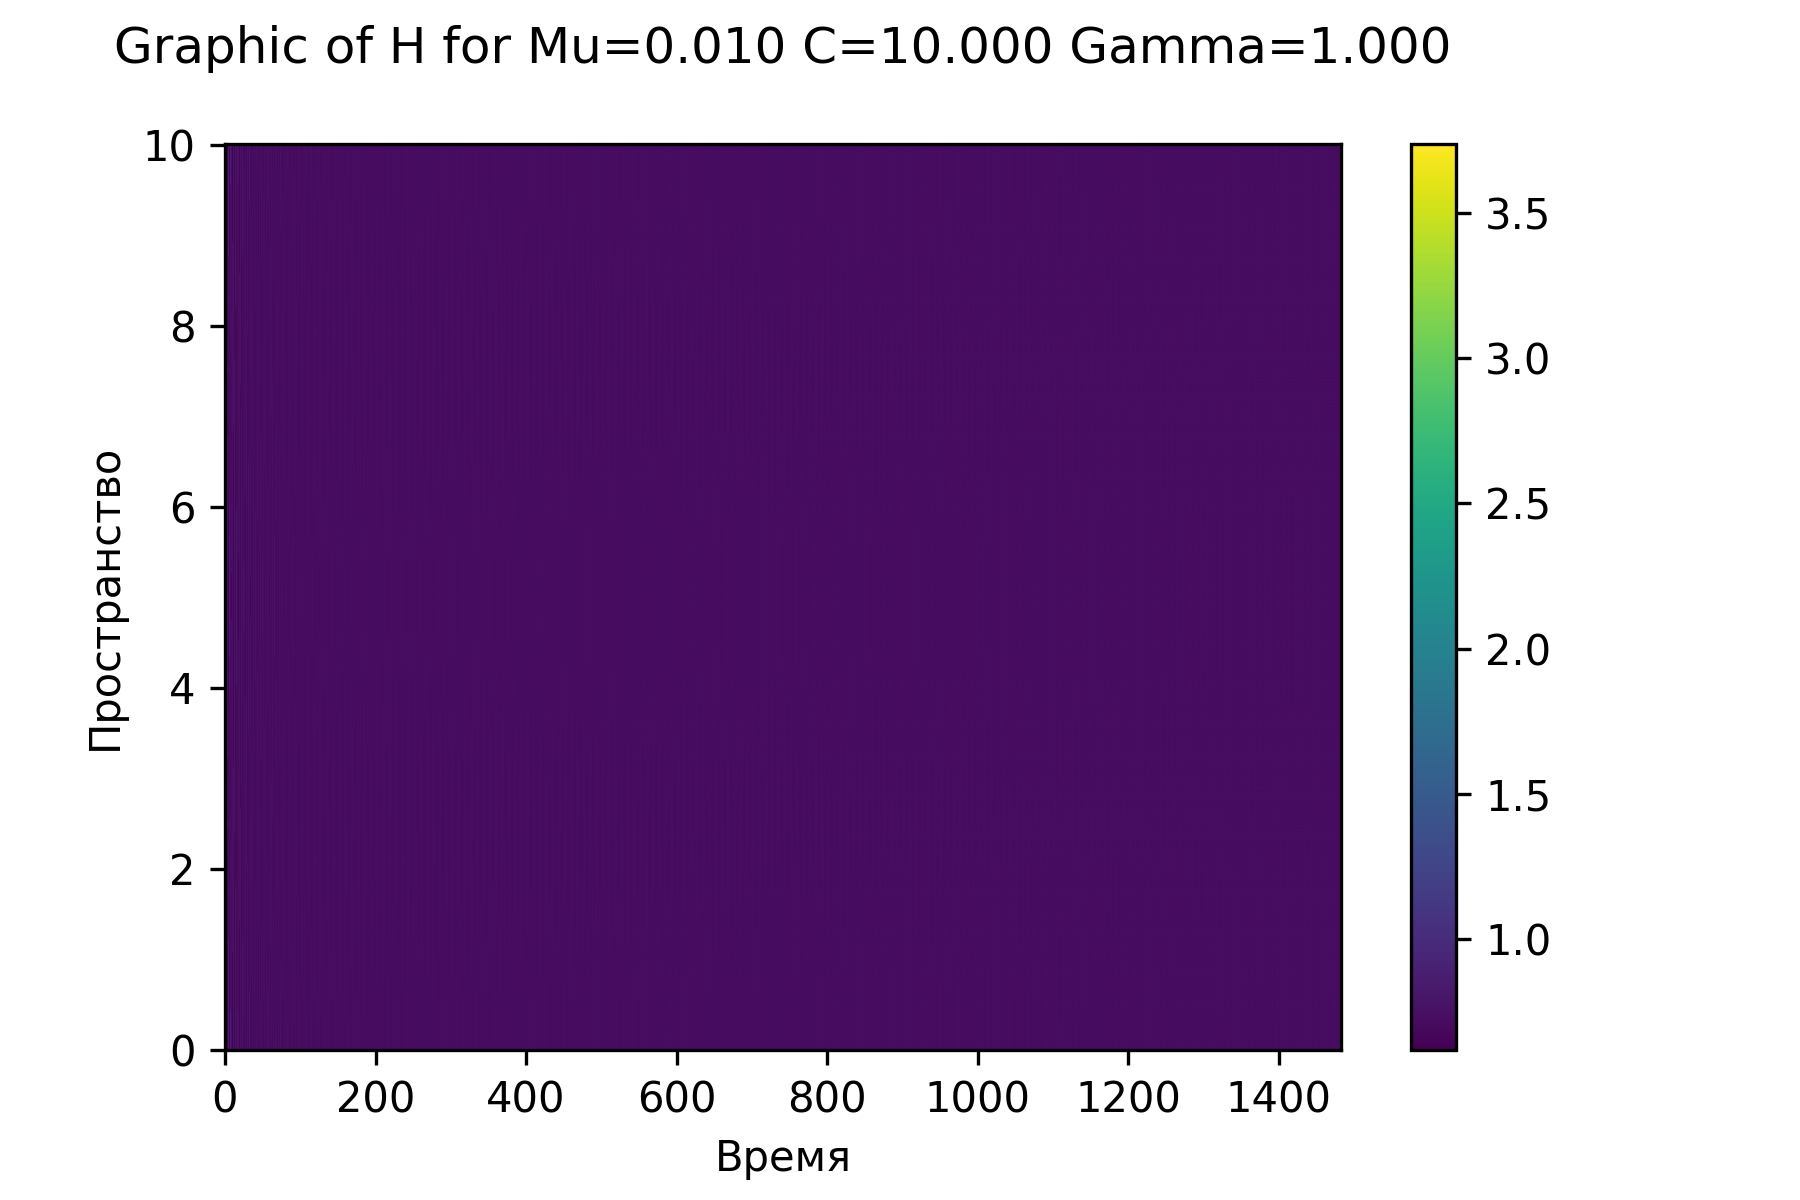
\includegraphics[scale=0.5]{../graphs_data_nonsmooth_1/value/Graph_H_mu0.010_C10.000_gamma1.000.png}
	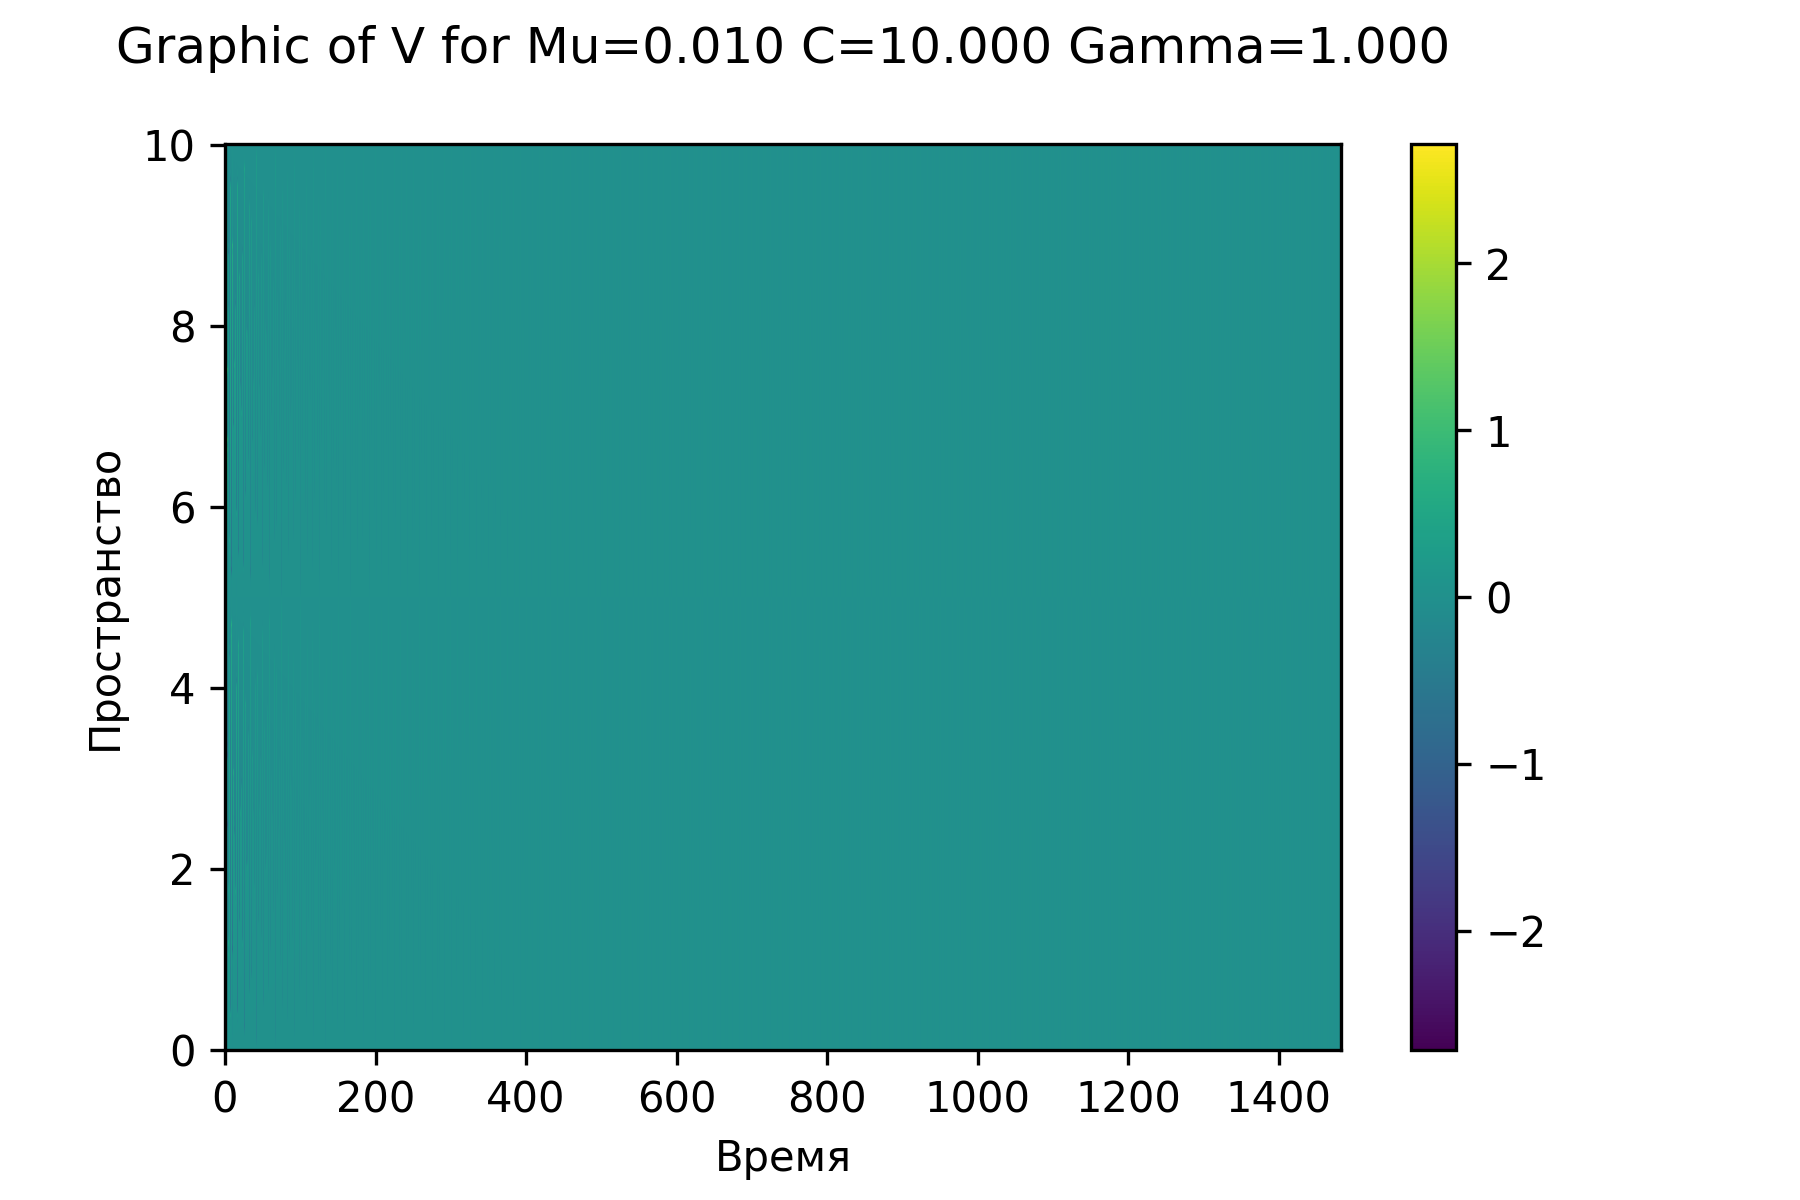
\includegraphics[scale=0.5]{../graphs_data_nonsmooth_1/value/Graph_V_mu0.010_C10.000_gamma1.000.png}	
	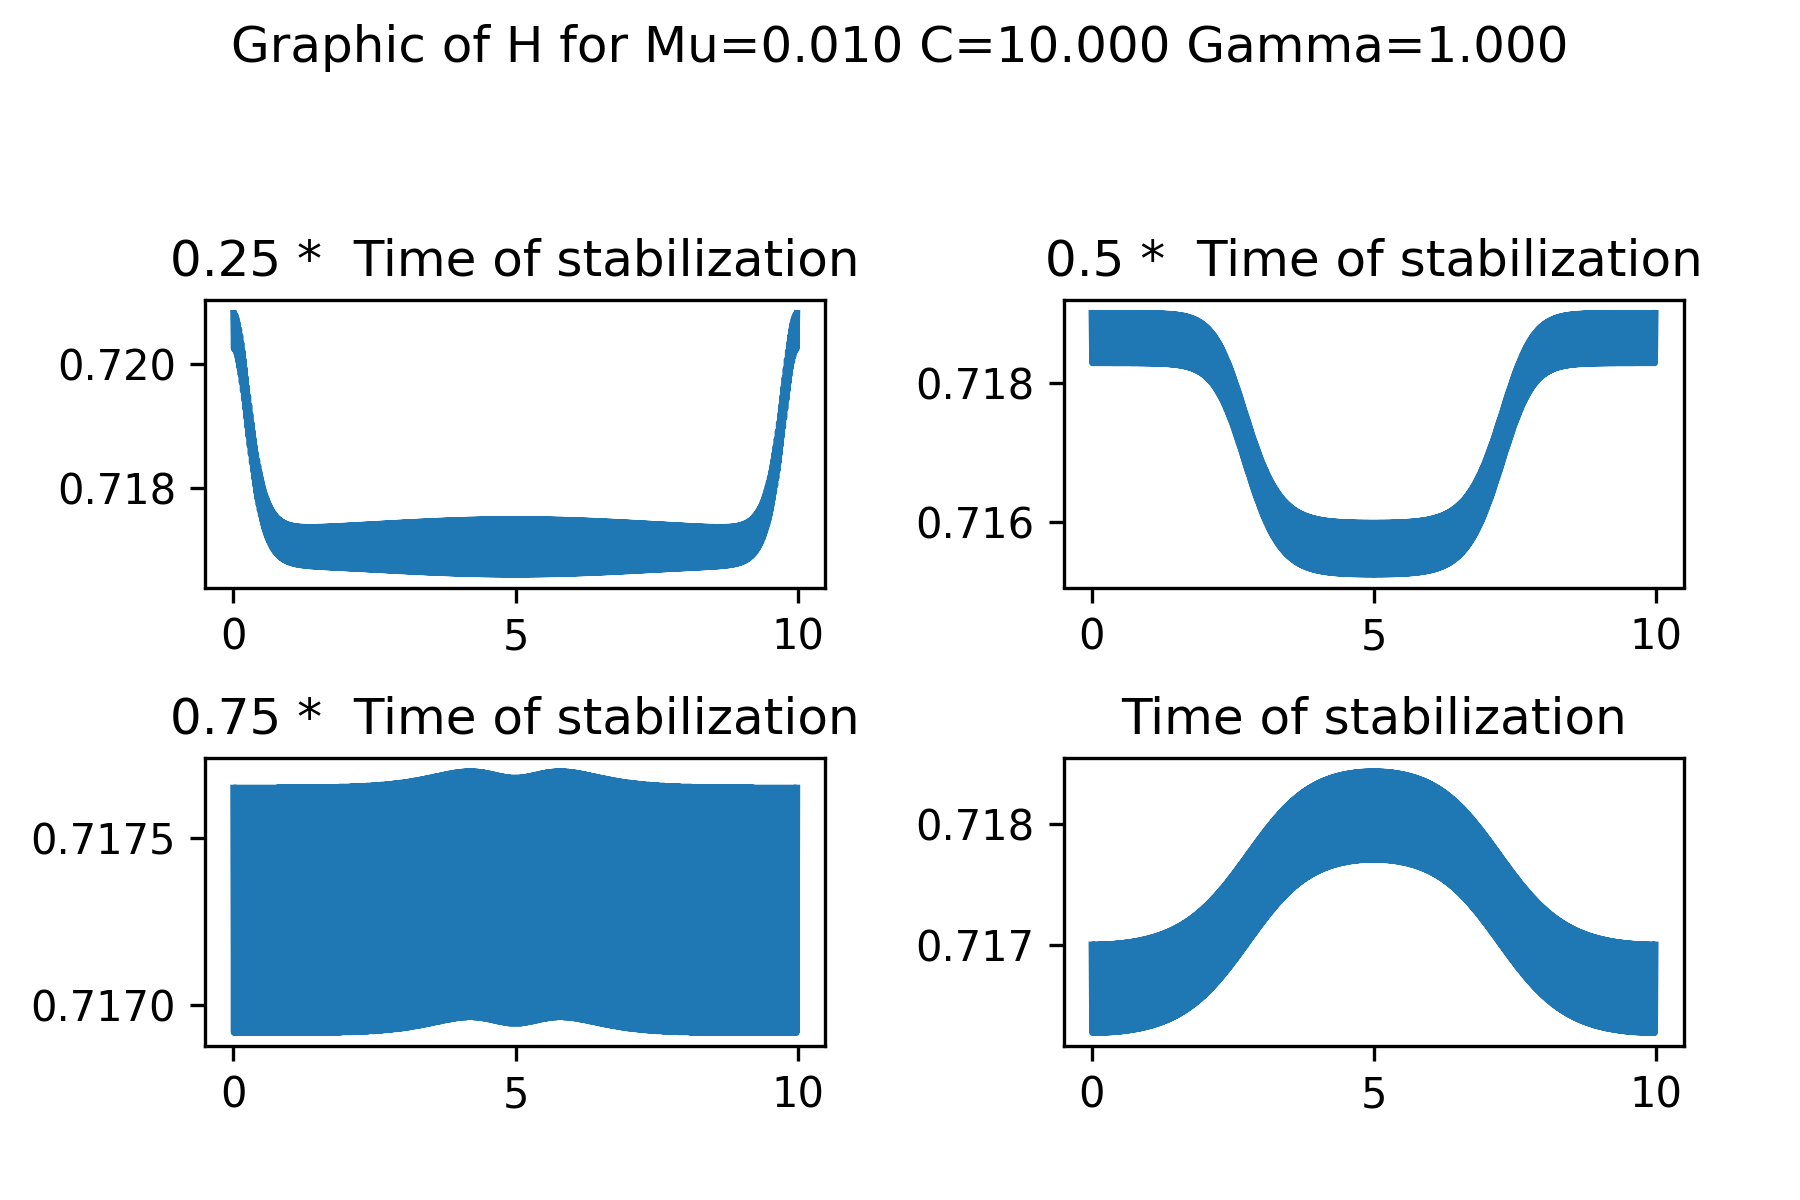
\includegraphics[scale=0.5]{../graphs_data_nonsmooth_1/slices/Graph_H_mu0.010_C10.000_gamma1.000.png}
	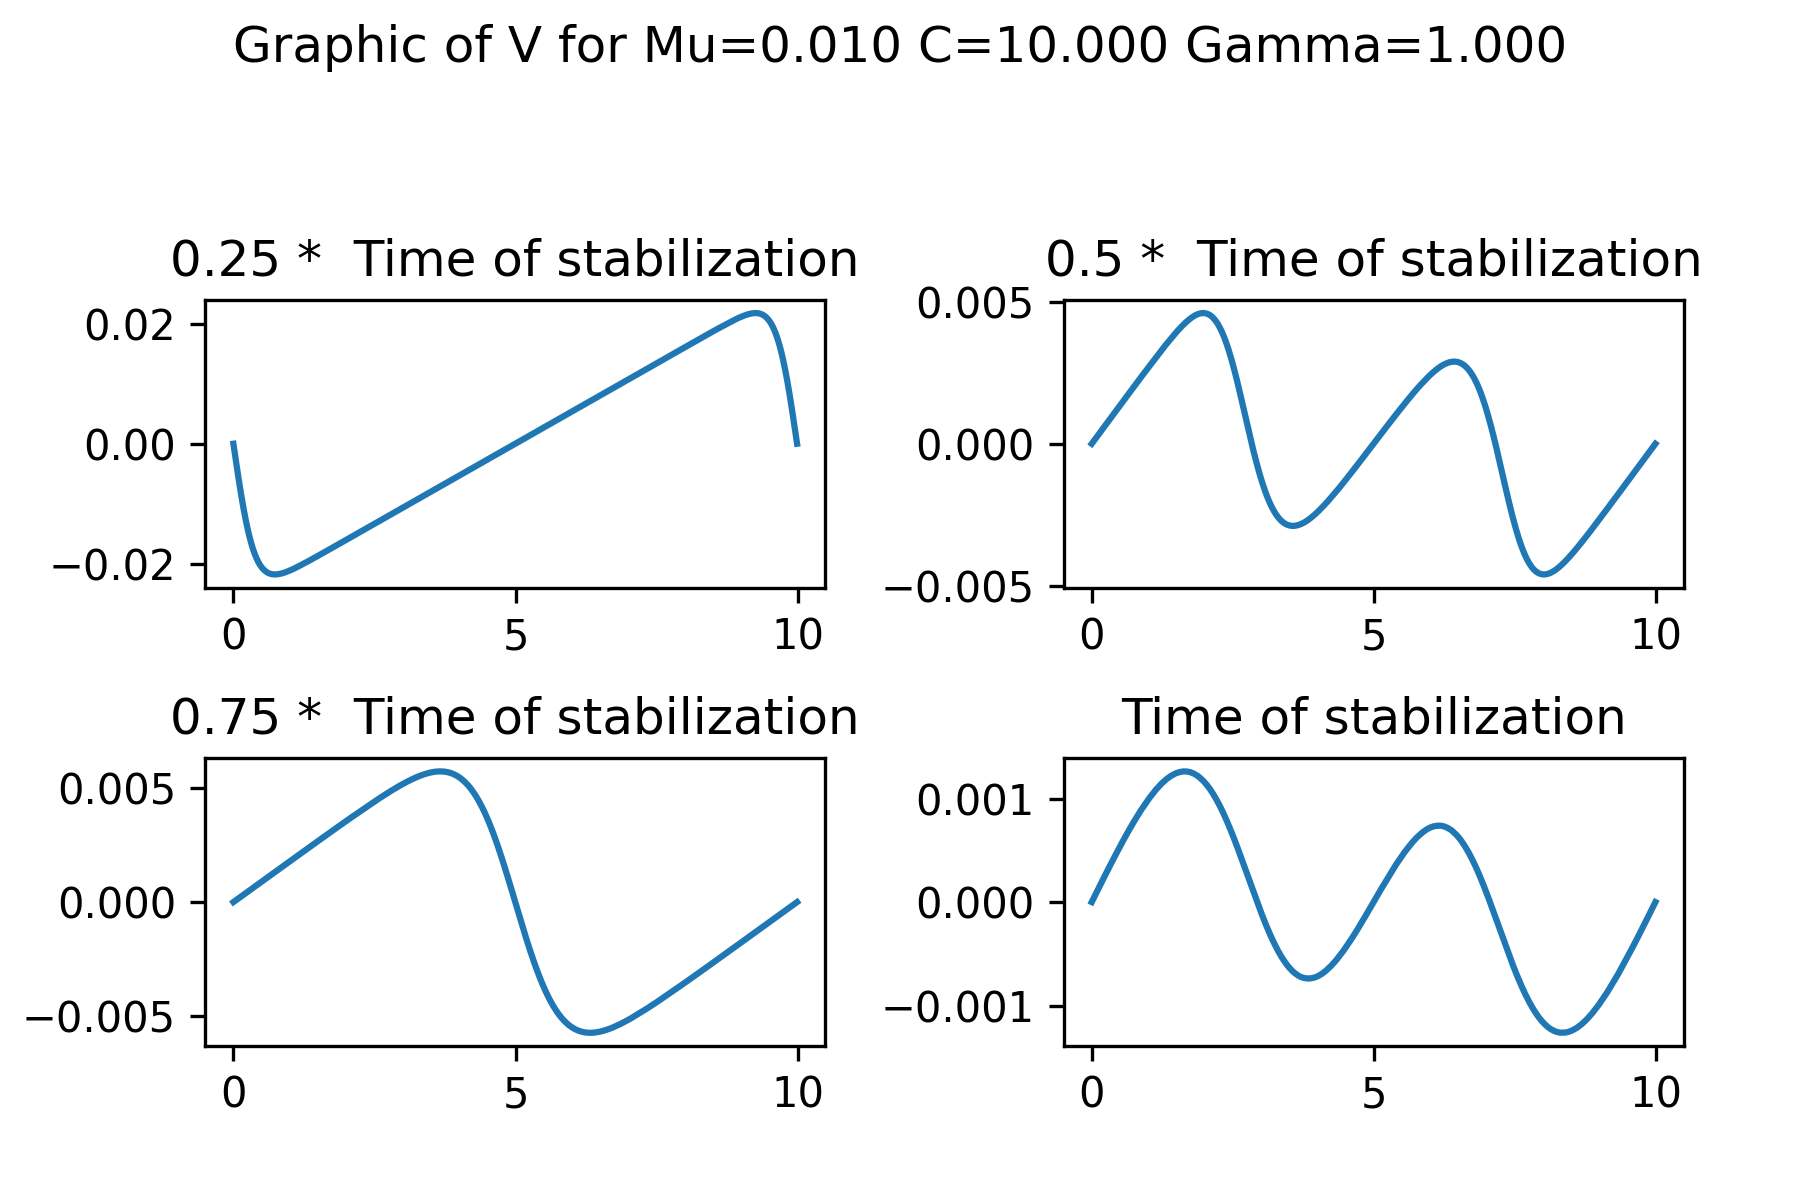
\includegraphics[scale=0.5]{../graphs_data_nonsmooth_1/slices/Graph_V_mu0.010_C10.000_gamma1.000.png}
\end{figure}

\begin{figure}[H]
	\centering
	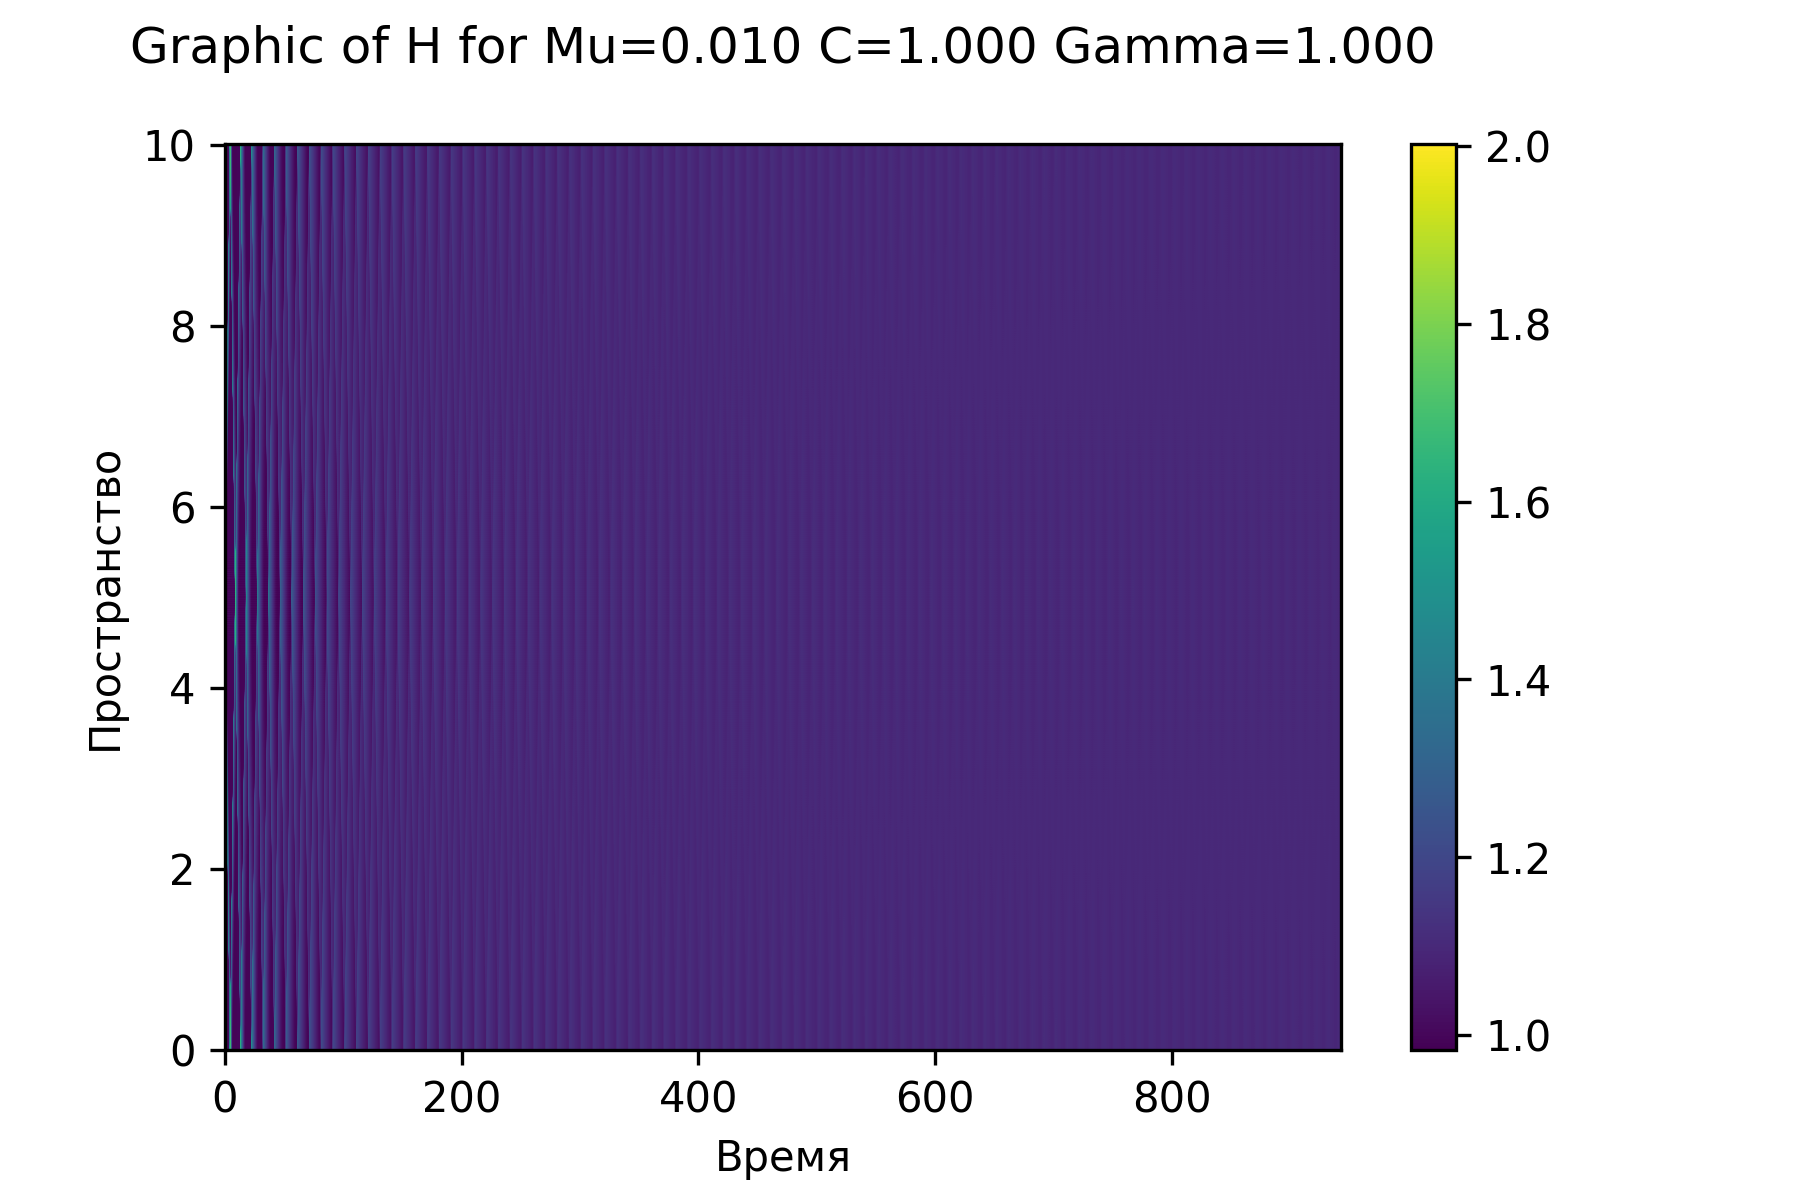
\includegraphics[scale=0.5]{../graphs_data_nonsmooth_1/value/Graph_H_mu0.010_C1.000_gamma1.000.png}
	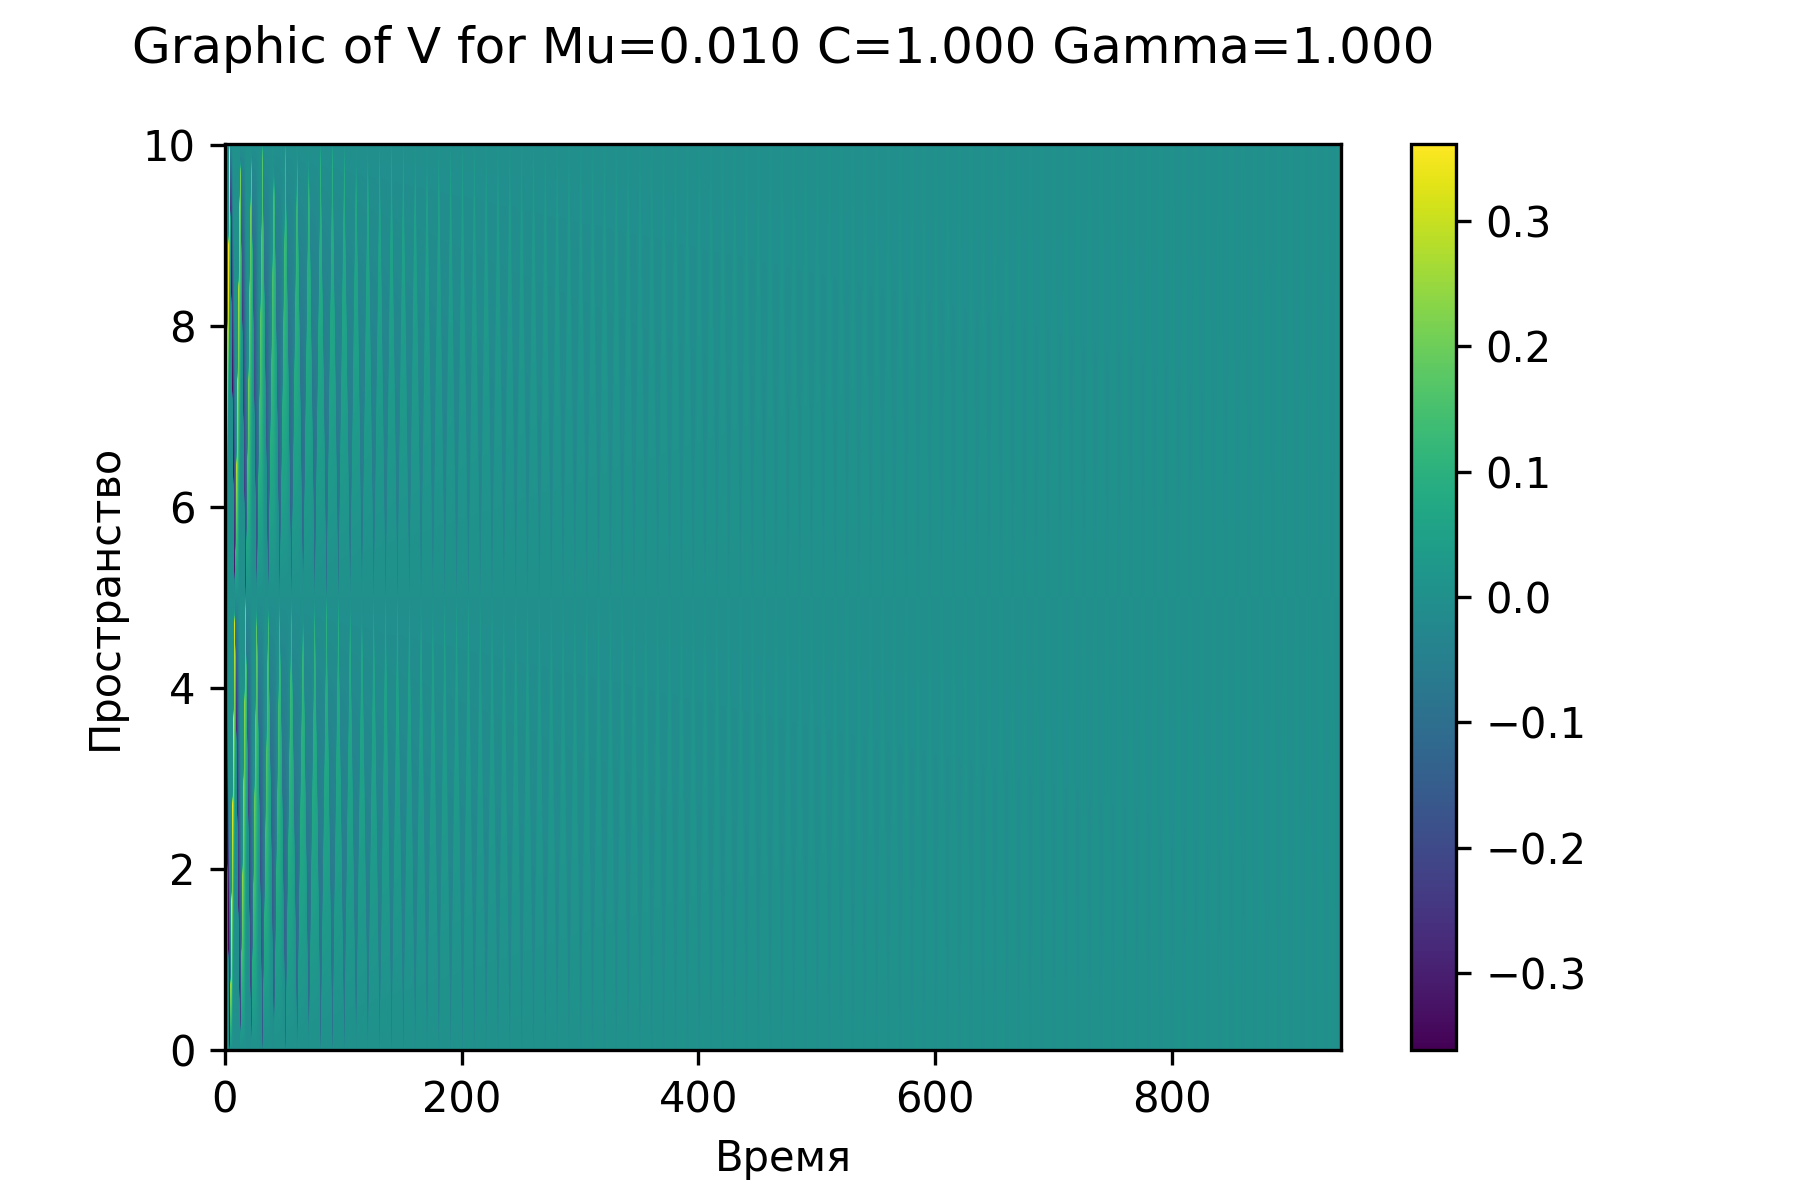
\includegraphics[scale=0.5]{../graphs_data_nonsmooth_1/value/Graph_V_mu0.010_C1.000_gamma1.000.png}	
	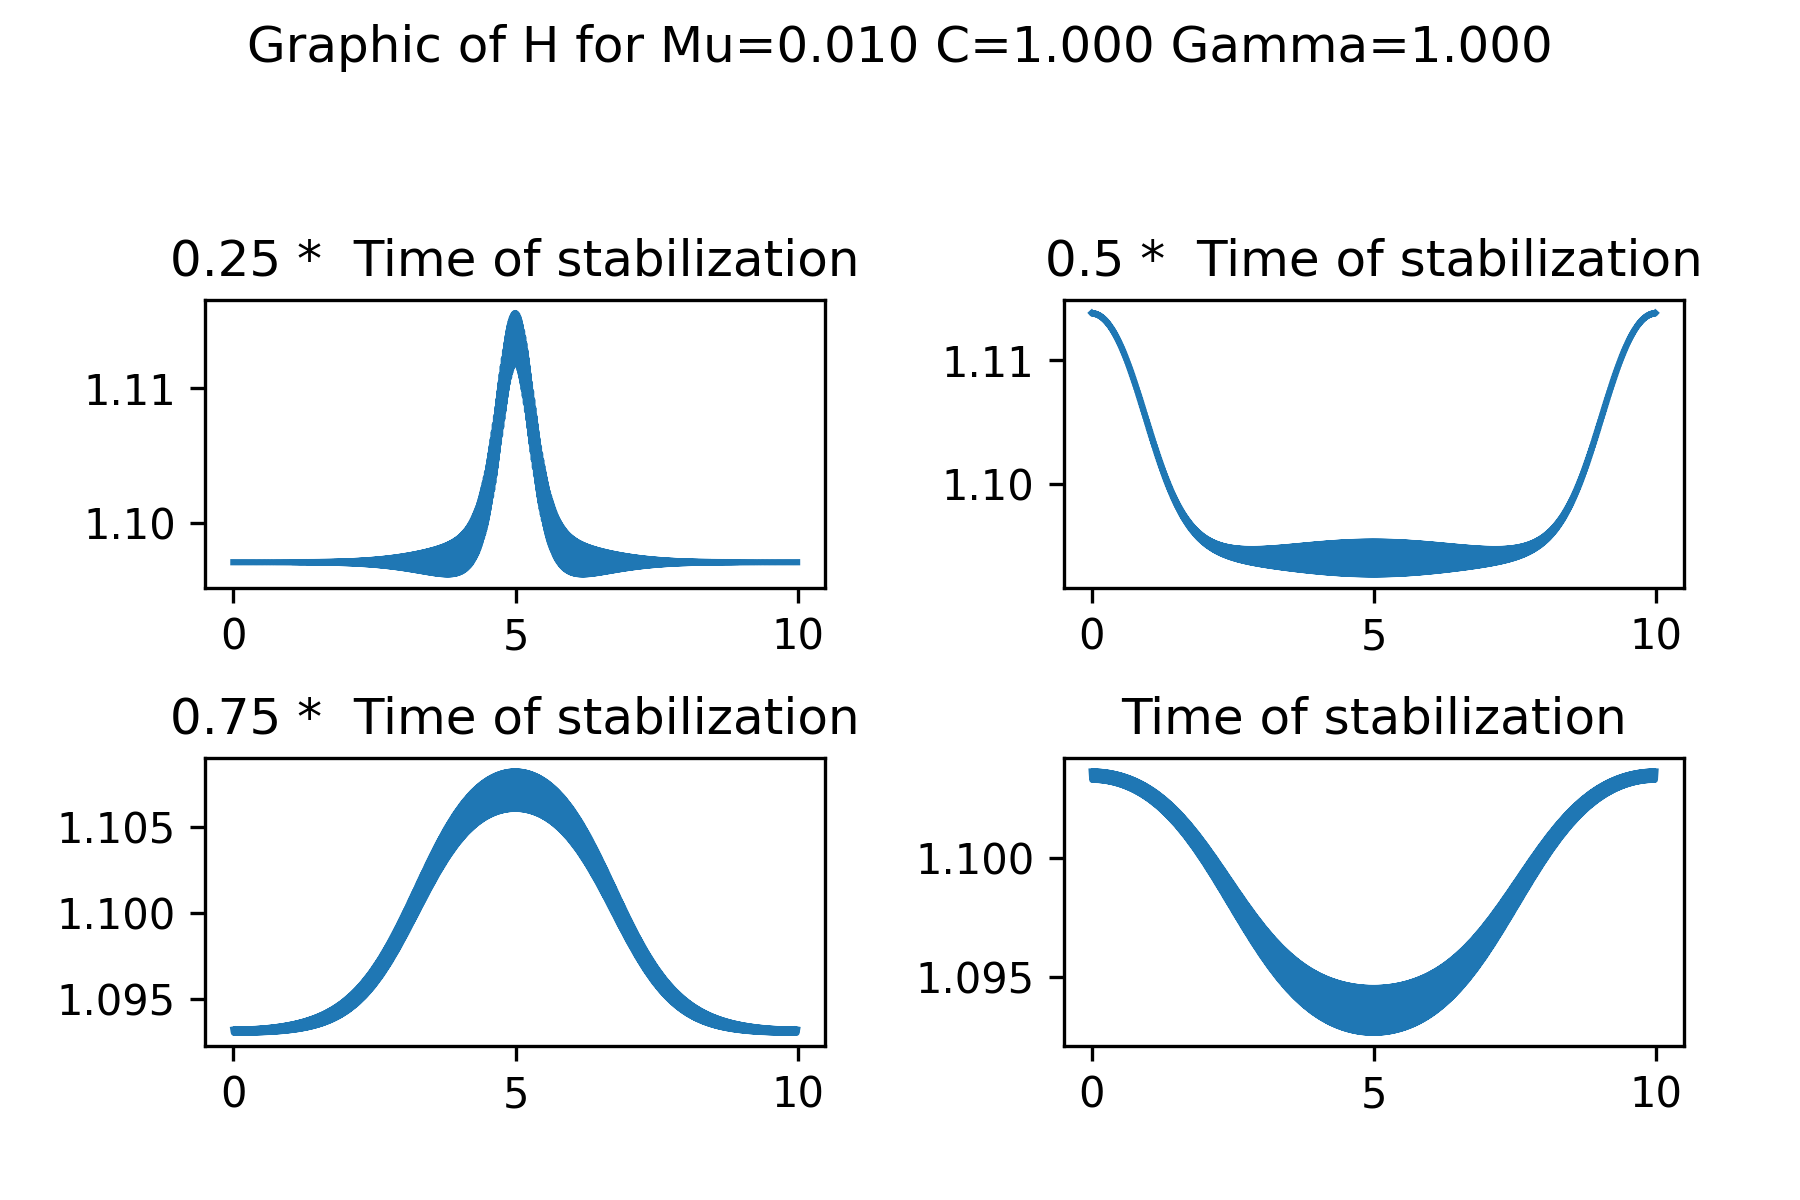
\includegraphics[scale=0.5]{../graphs_data_nonsmooth_1/slices/Graph_H_mu0.010_C1.000_gamma1.000.png}
	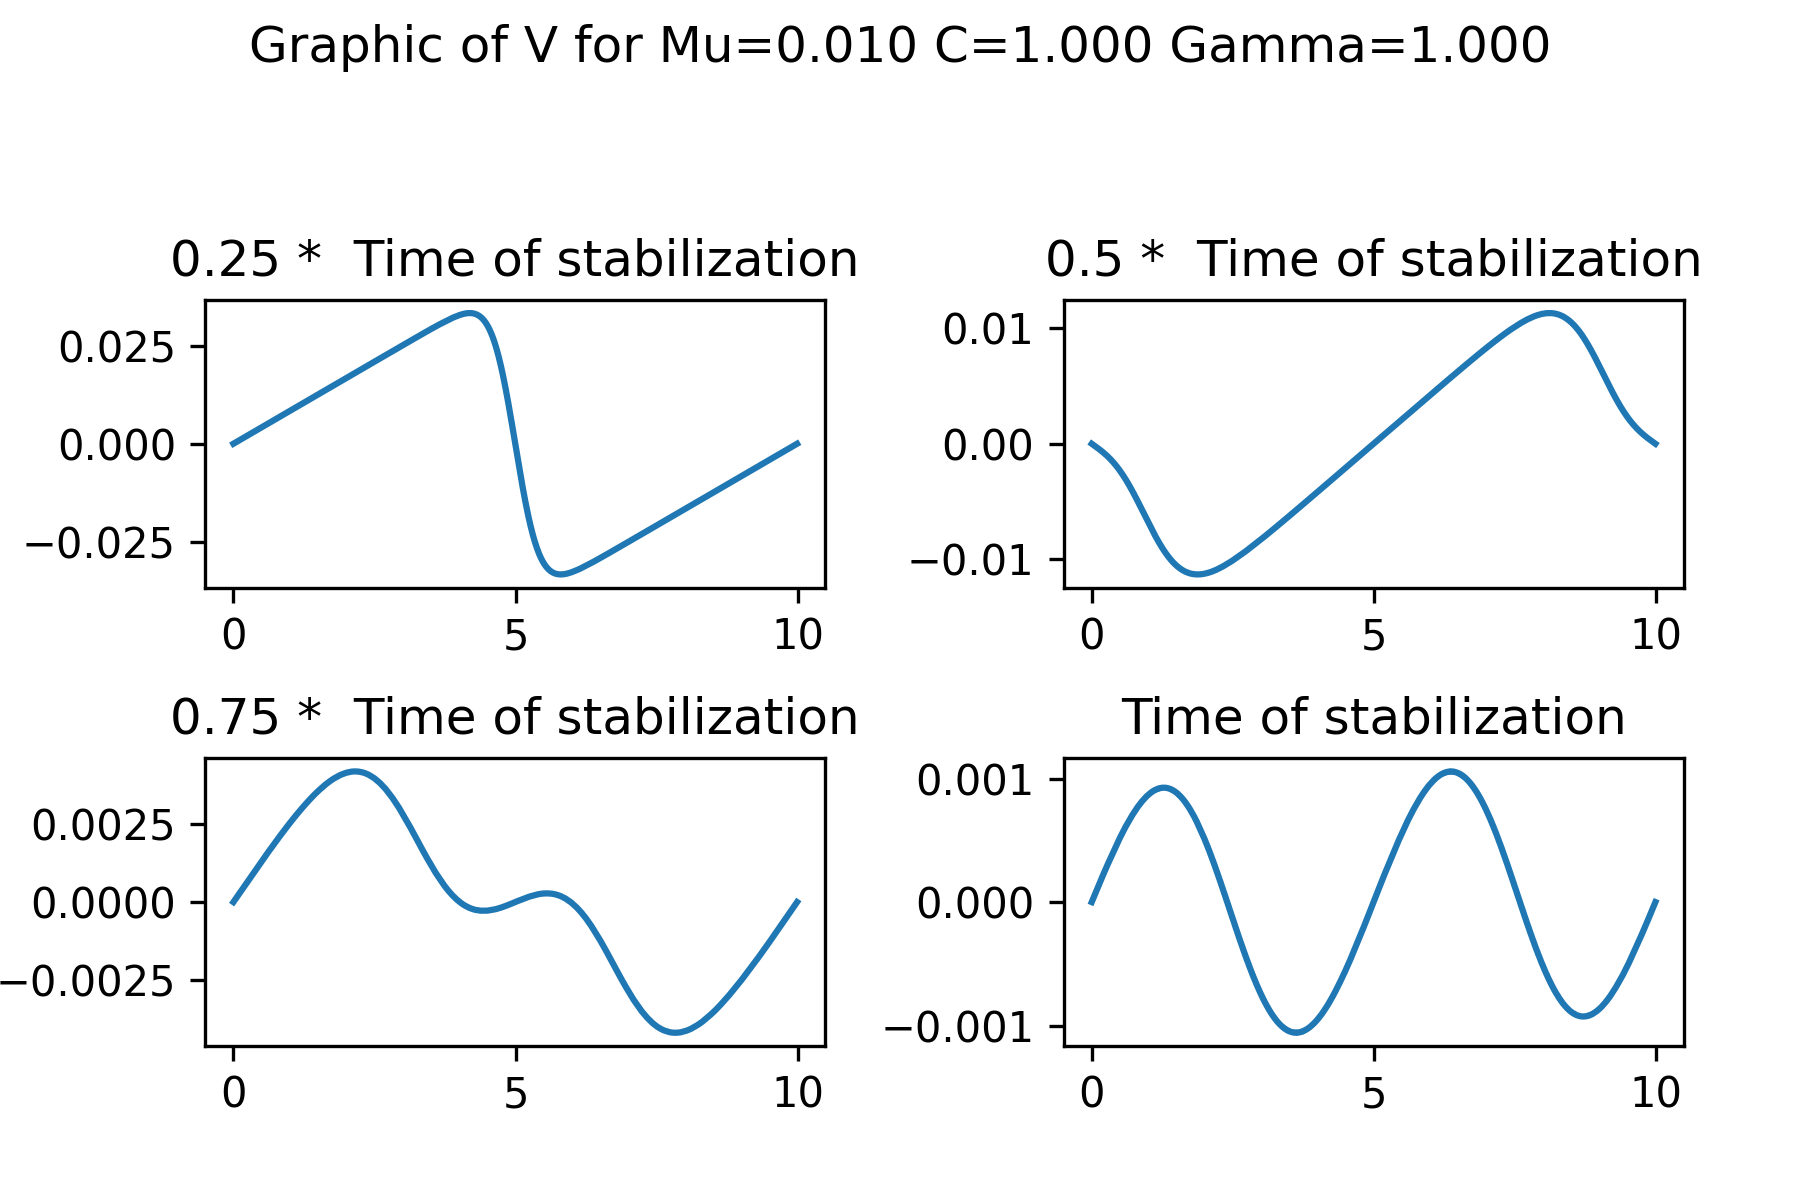
\includegraphics[scale=0.5]{../graphs_data_nonsmooth_1/slices/Graph_V_mu0.010_C1.000_gamma1.000.png}
\end{figure}

\begin{figure}[H]
	\centering
	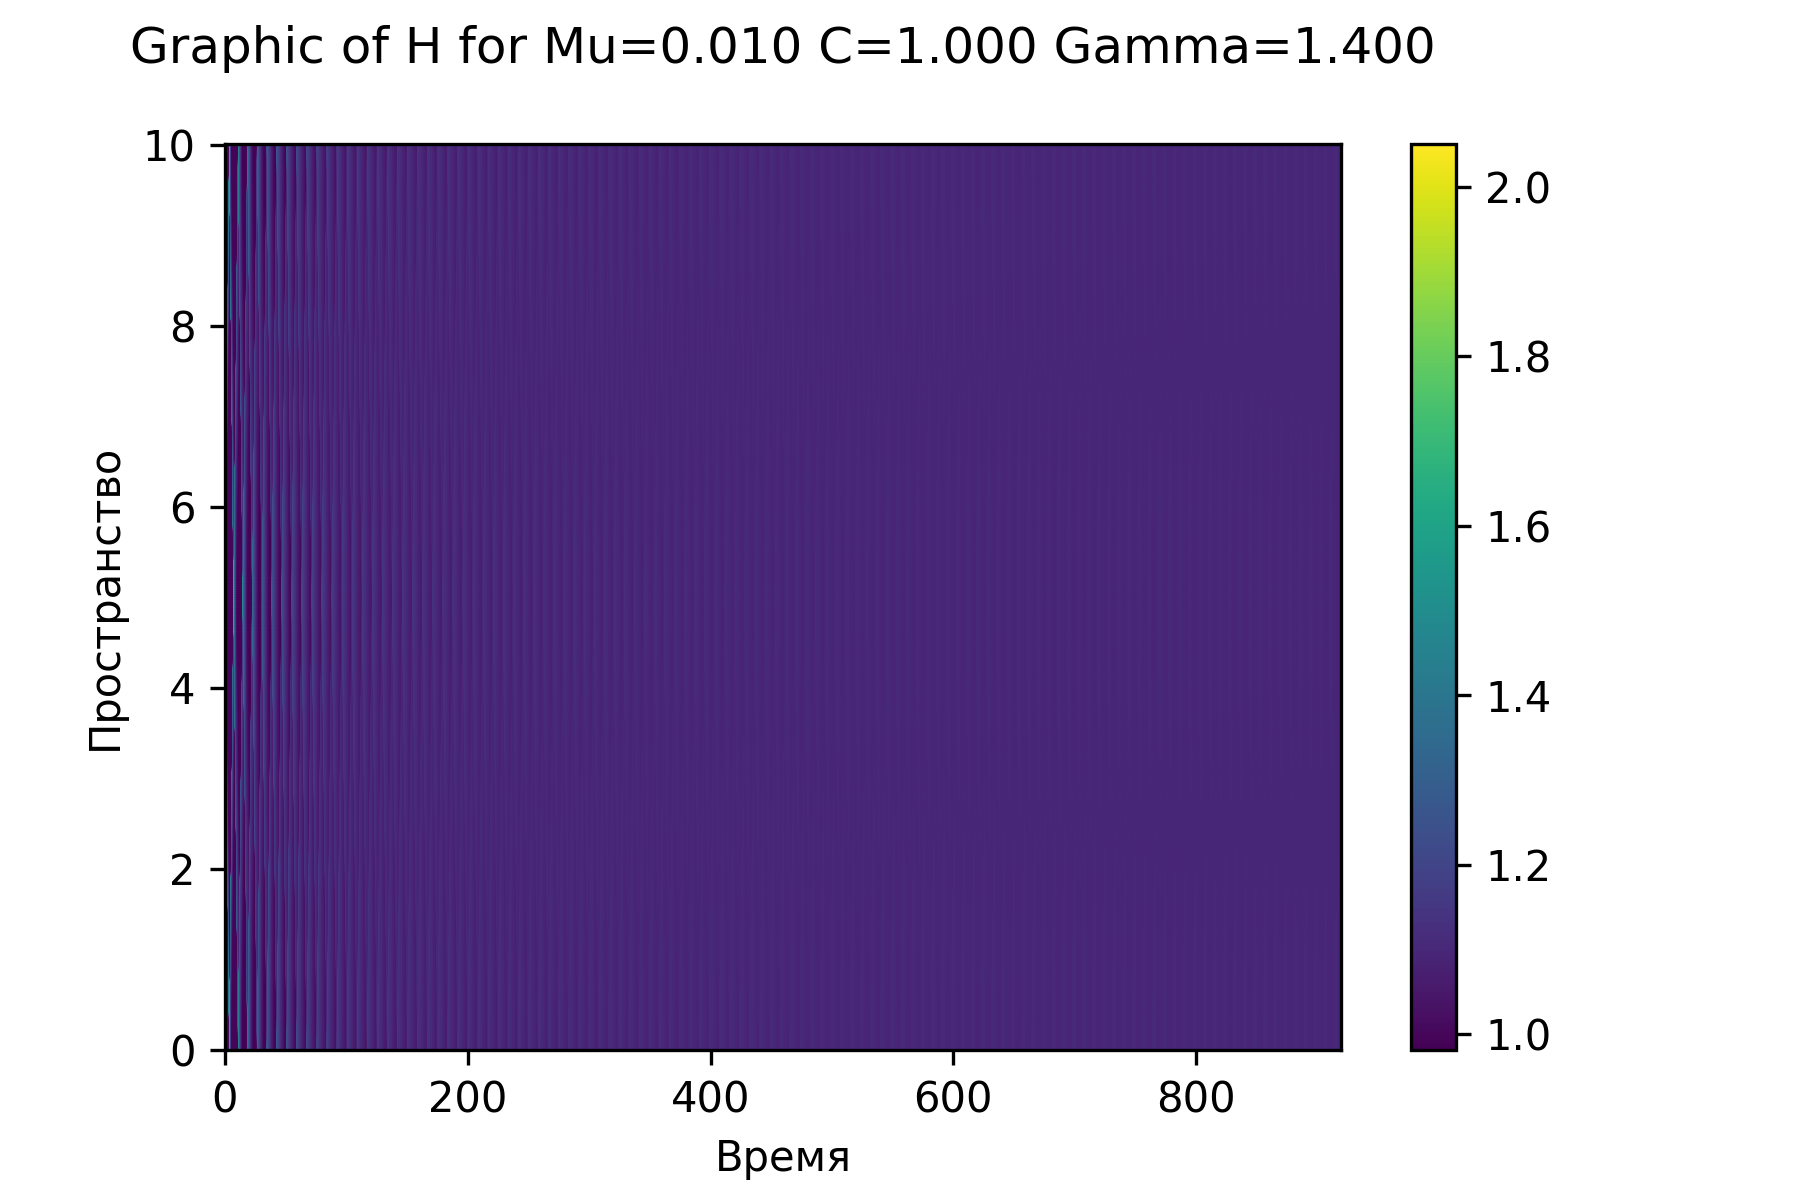
\includegraphics[scale=0.5]{../graphs_data_nonsmooth_1/value/Graph_H_mu0.010_C1.000_gamma1.400.png}
	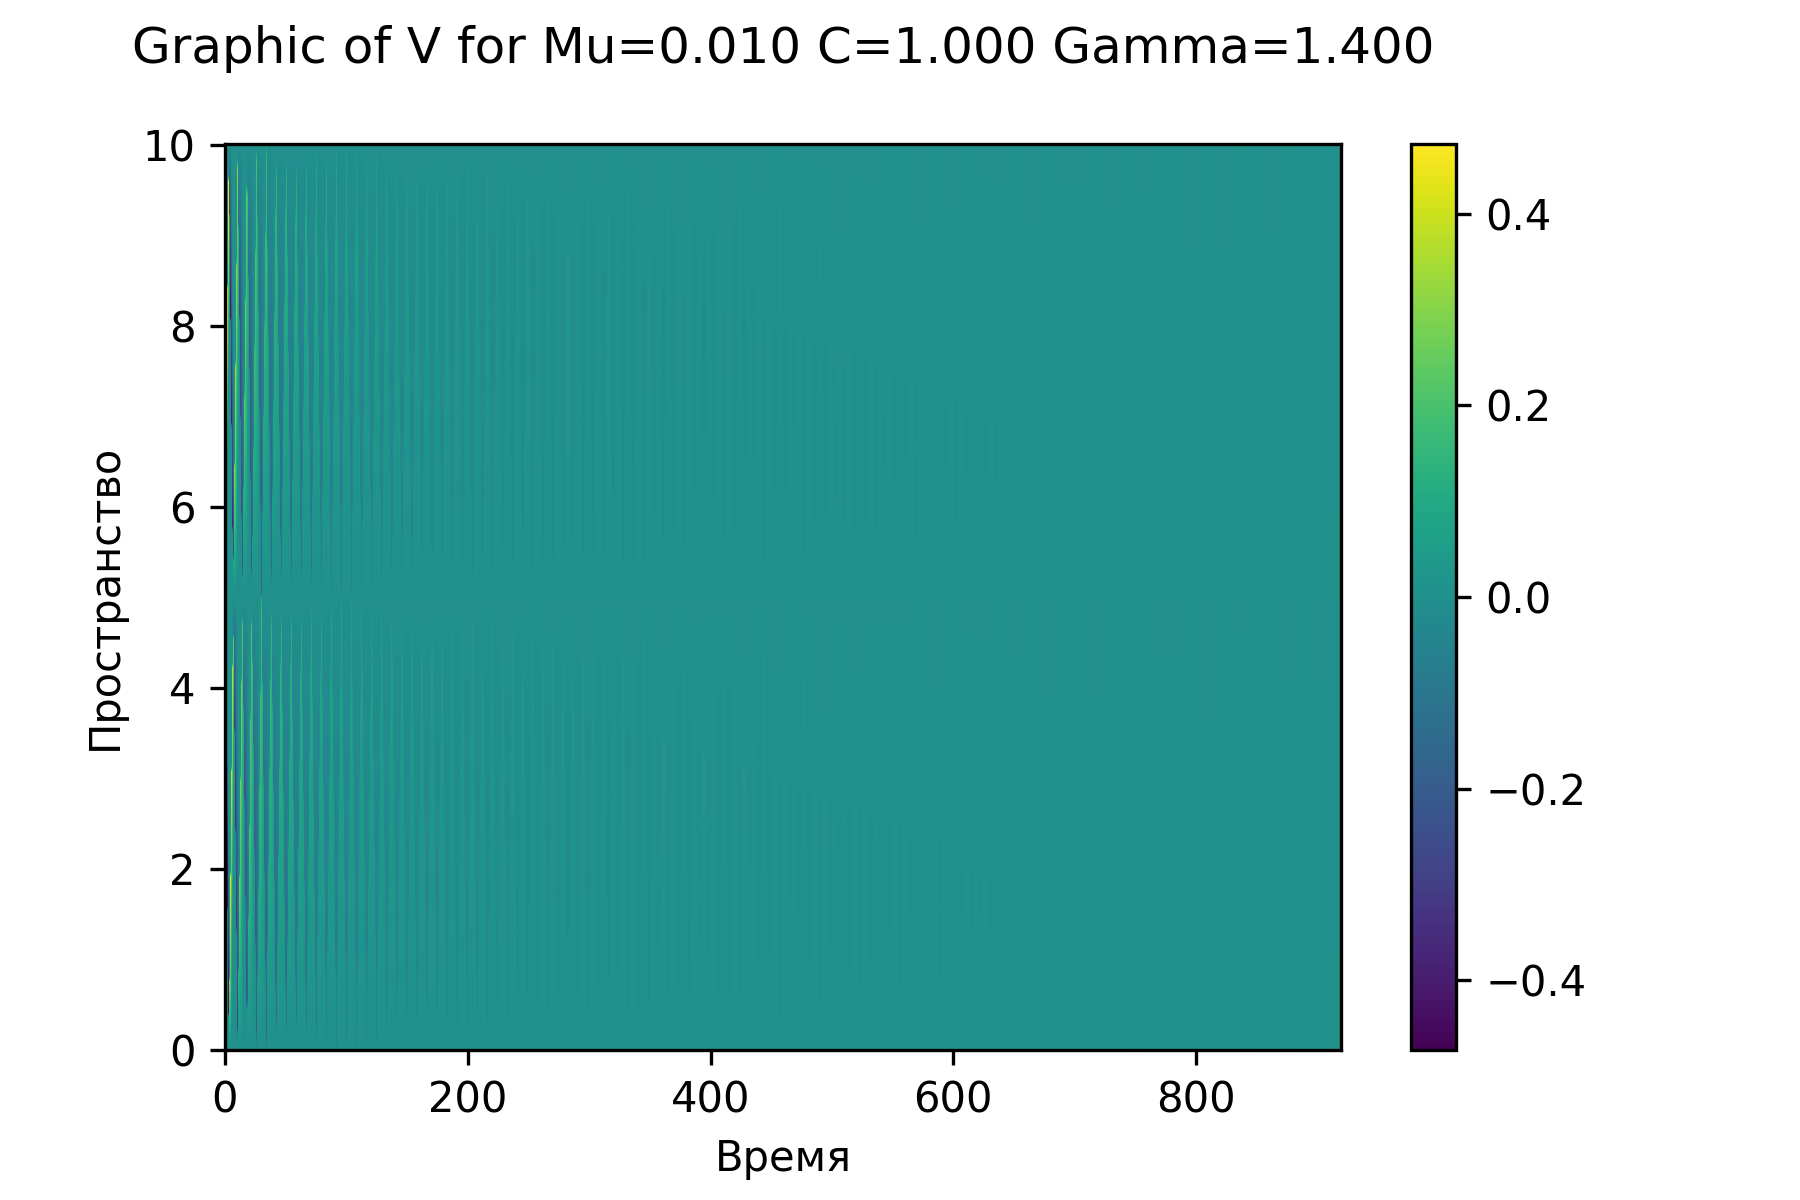
\includegraphics[scale=0.5]{../graphs_data_nonsmooth_1/value/Graph_V_mu0.010_C1.000_gamma1.400.png}	
	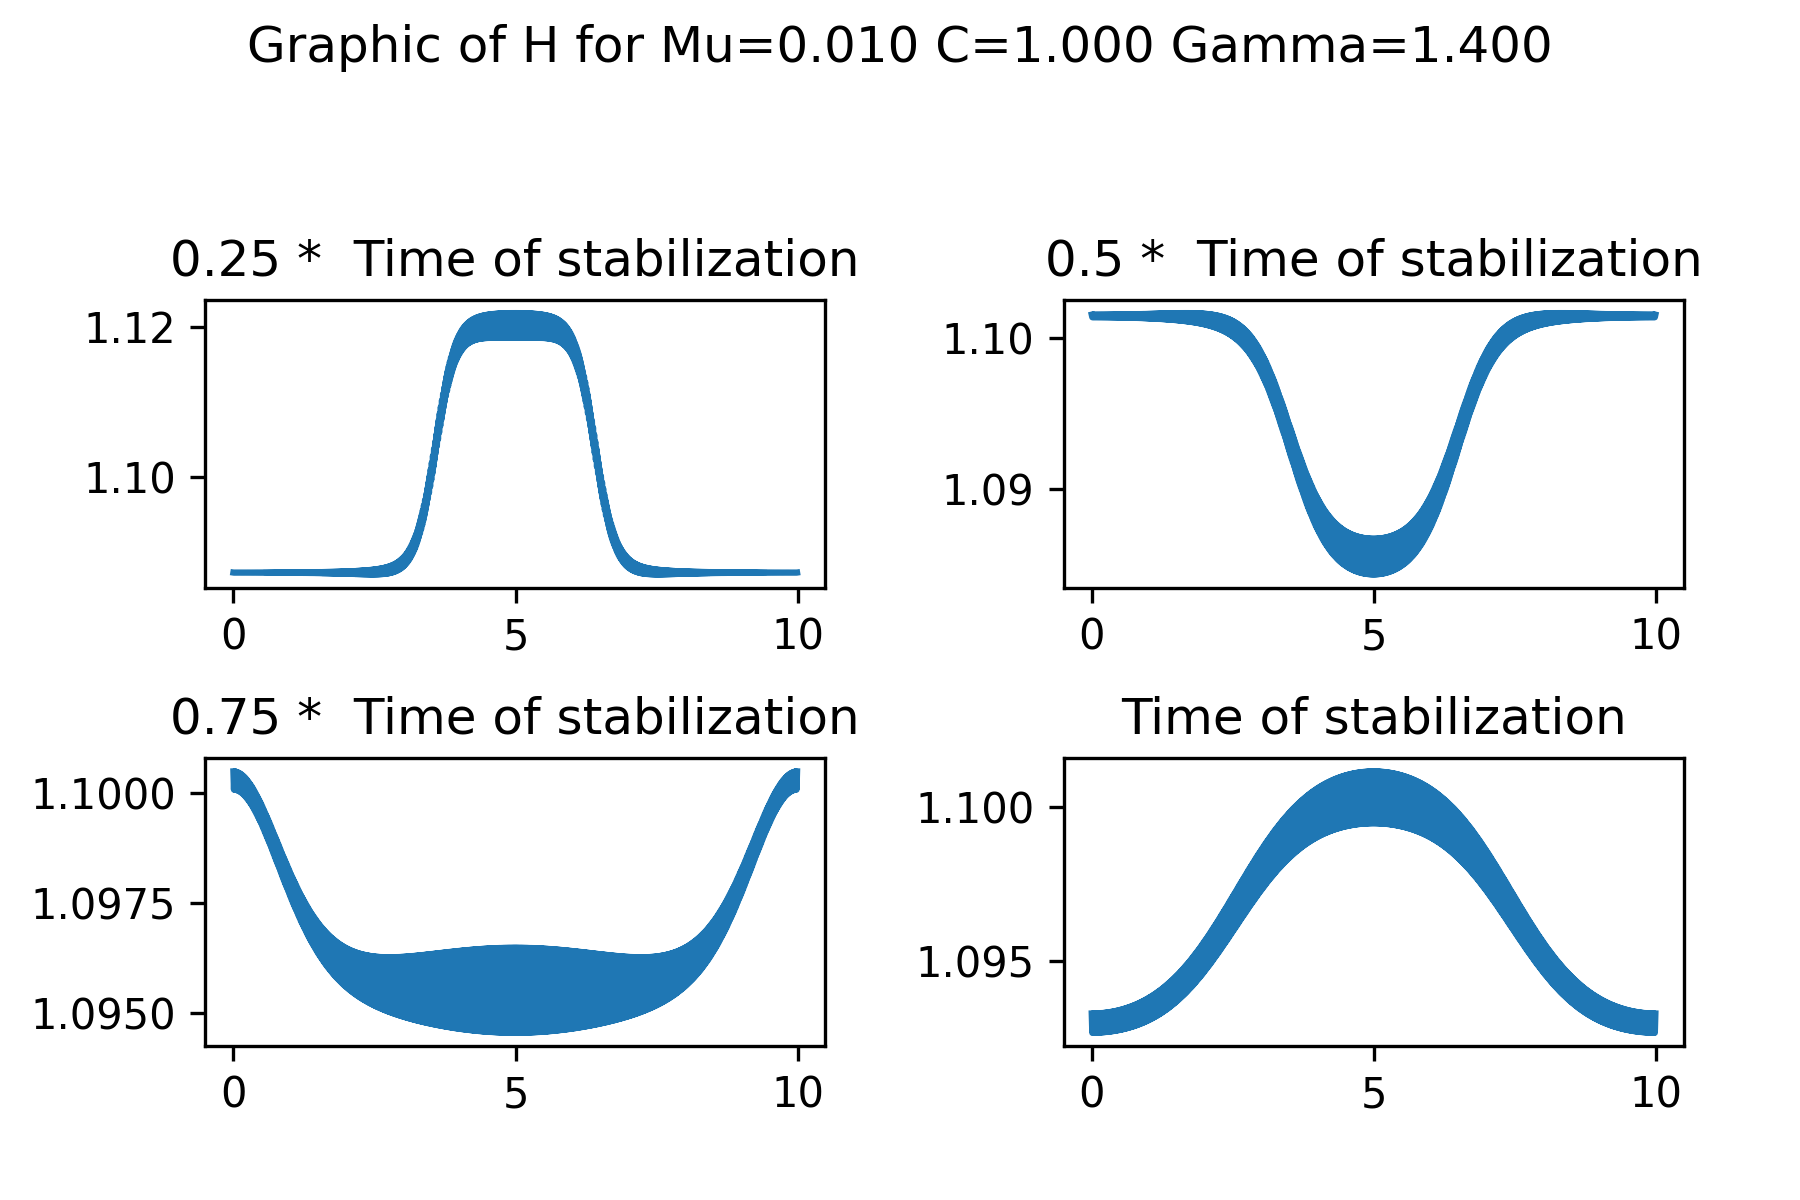
\includegraphics[scale=0.5]{../graphs_data_nonsmooth_1/slices/Graph_H_mu0.010_C1.000_gamma1.400.png}
	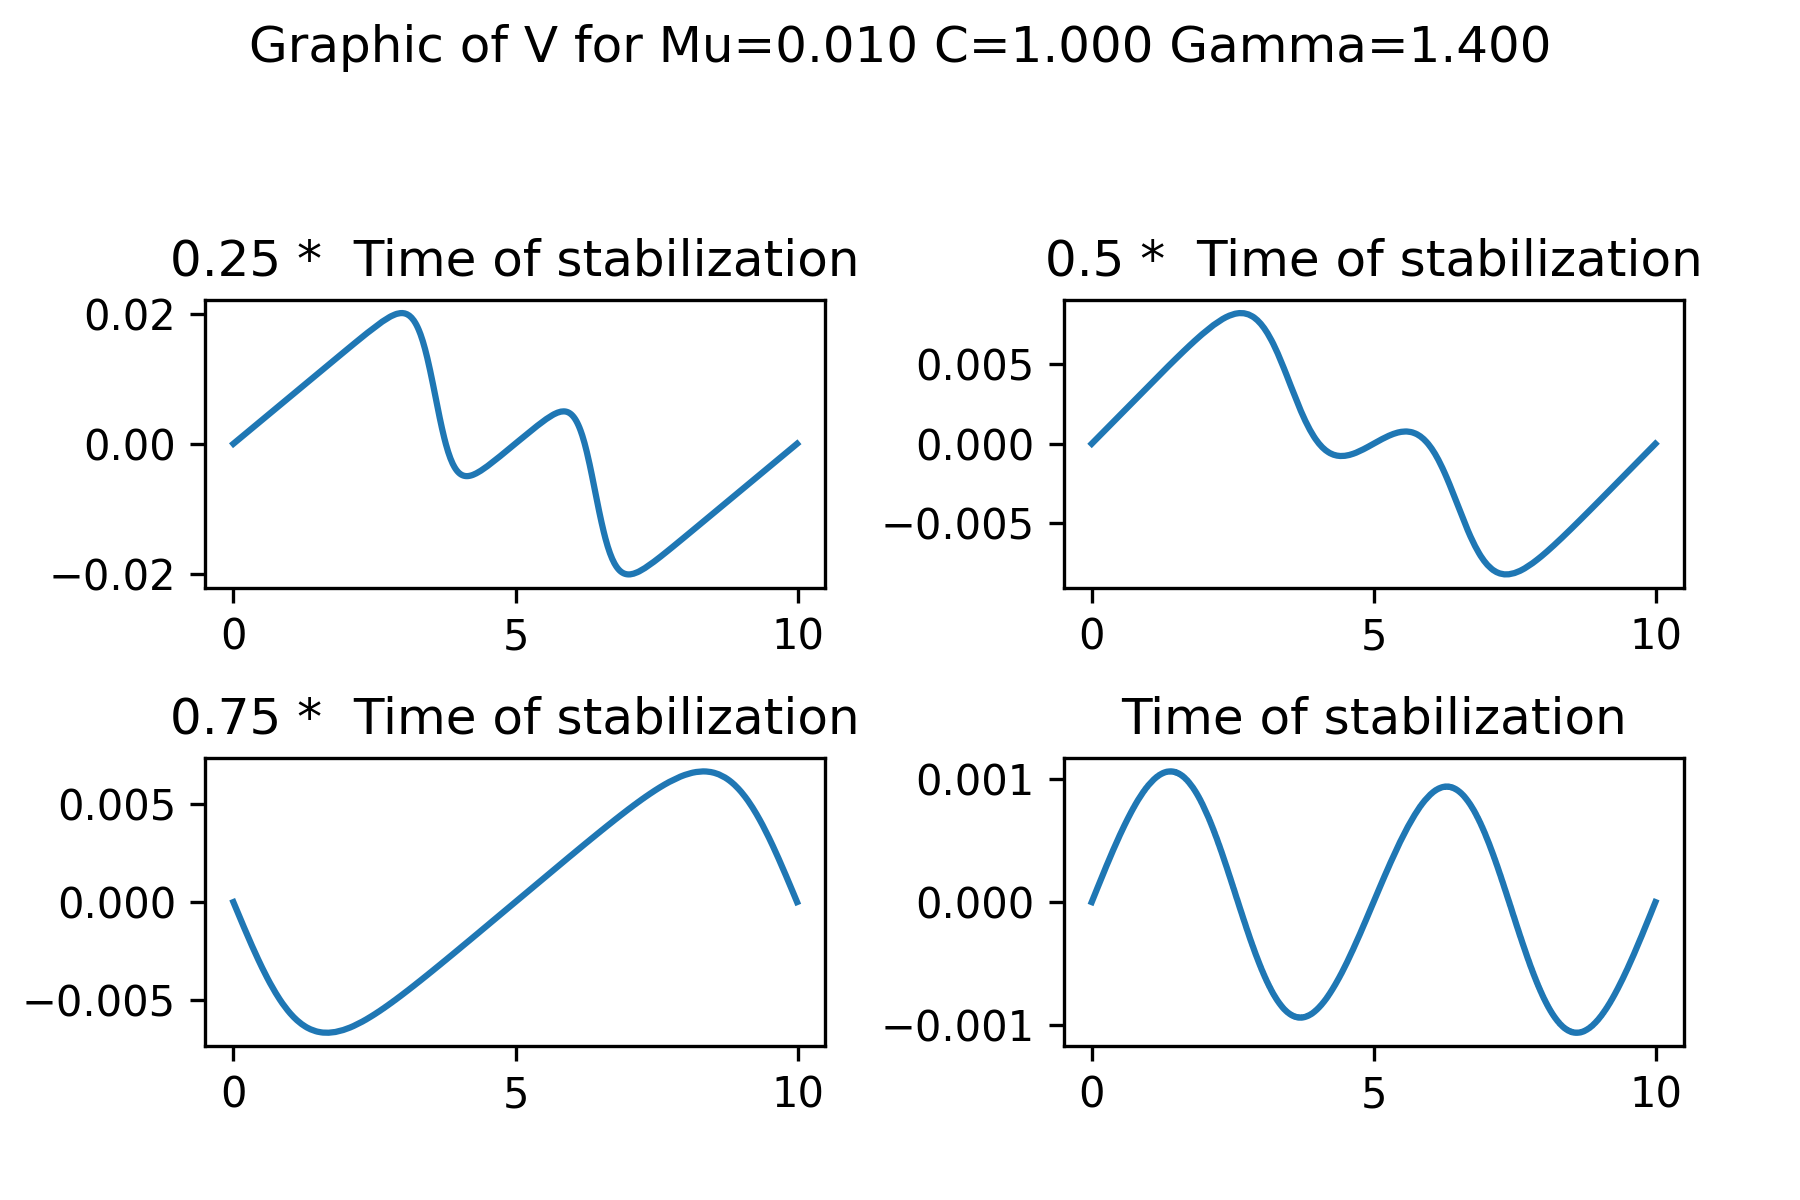
\includegraphics[scale=0.5]{../graphs_data_nonsmooth_1/slices/Graph_V_mu0.010_C1.000_gamma1.400.png}
\end{figure}

\begin{figure}[H]
	\centering
	\includegraphics[scale=0.5]{../graphs_data_nonsmooth_1/value/Graph_H_mu0.100_C10.000_gamma1.000.png}
	\includegraphics[scale=0.5]{../graphs_data_nonsmooth_1/value/Graph_V_mu0.100_C10.000_gamma1.000.png}	
	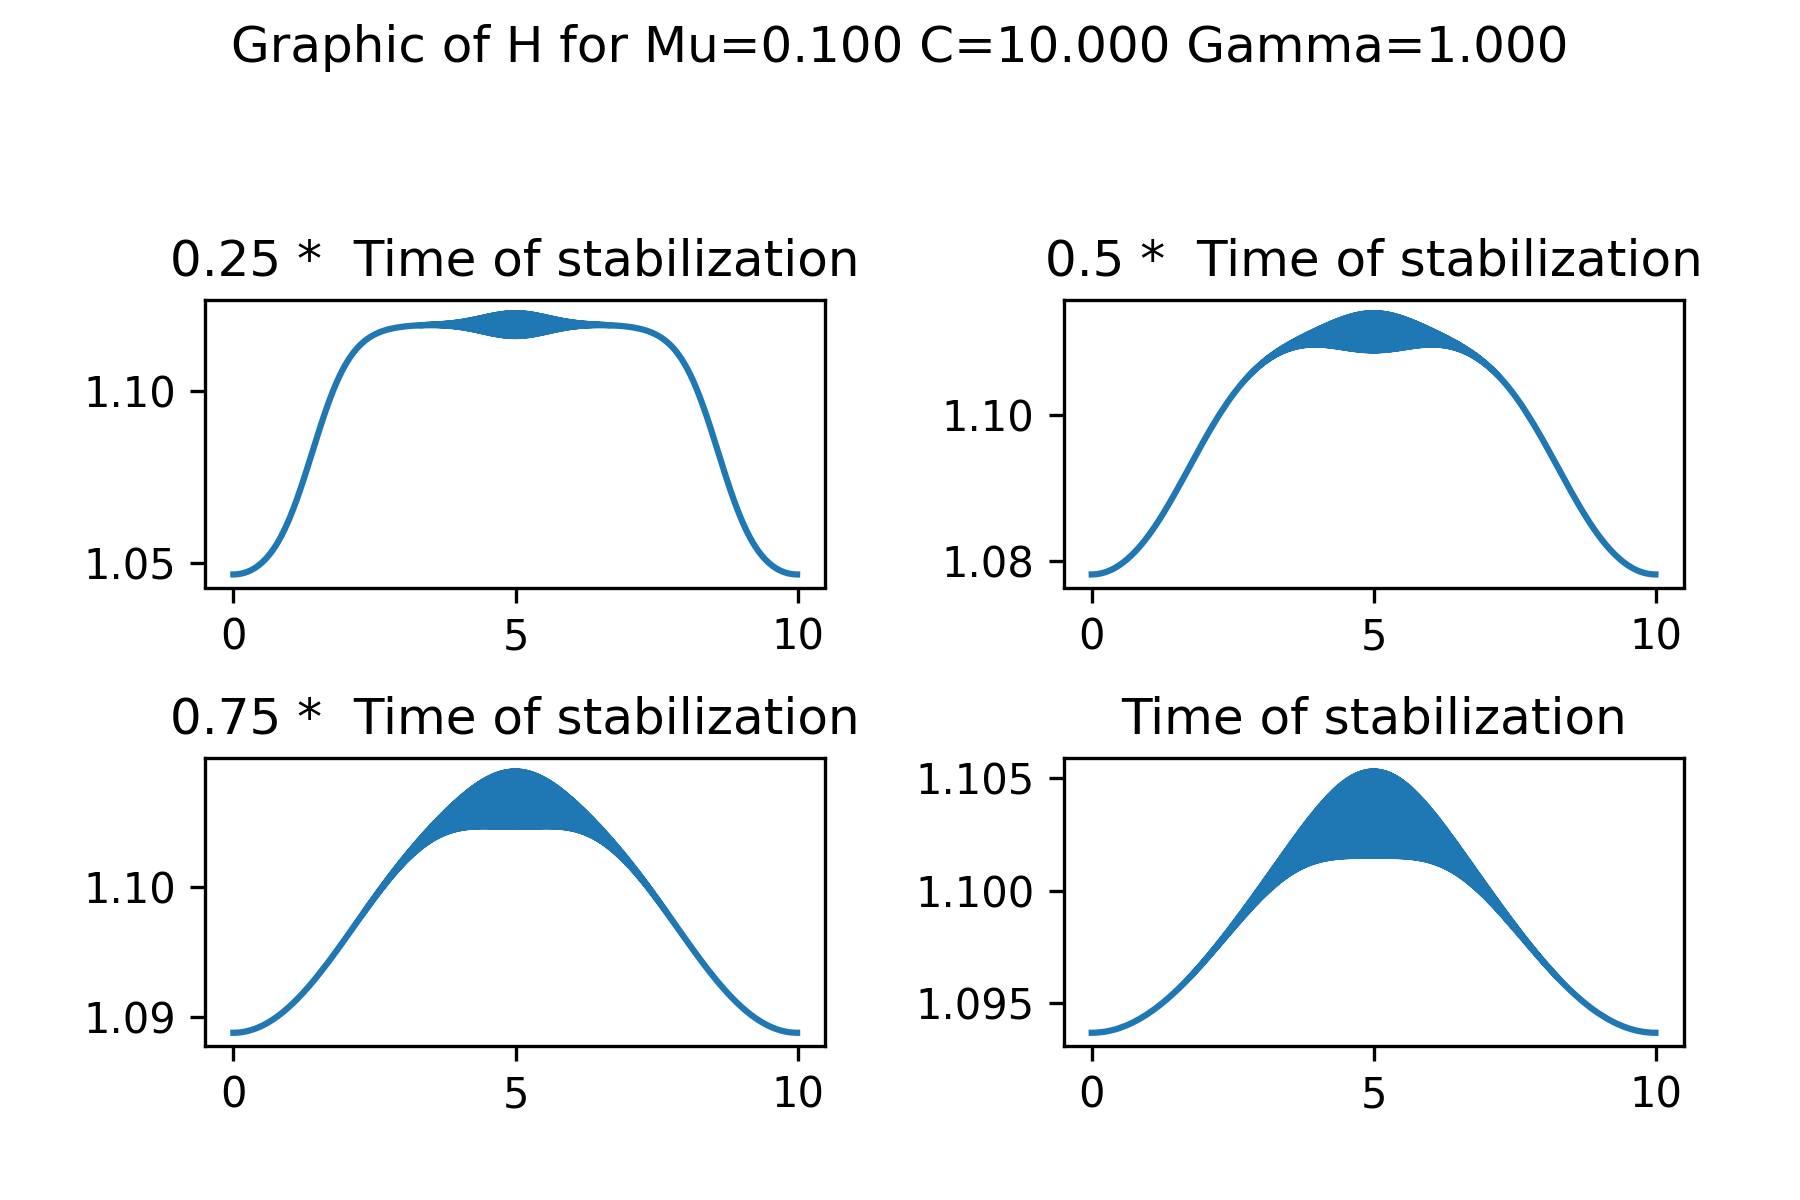
\includegraphics[scale=0.5]{../graphs_data_nonsmooth_1/slices/Graph_H_mu0.100_C10.000_gamma1.000.png}
	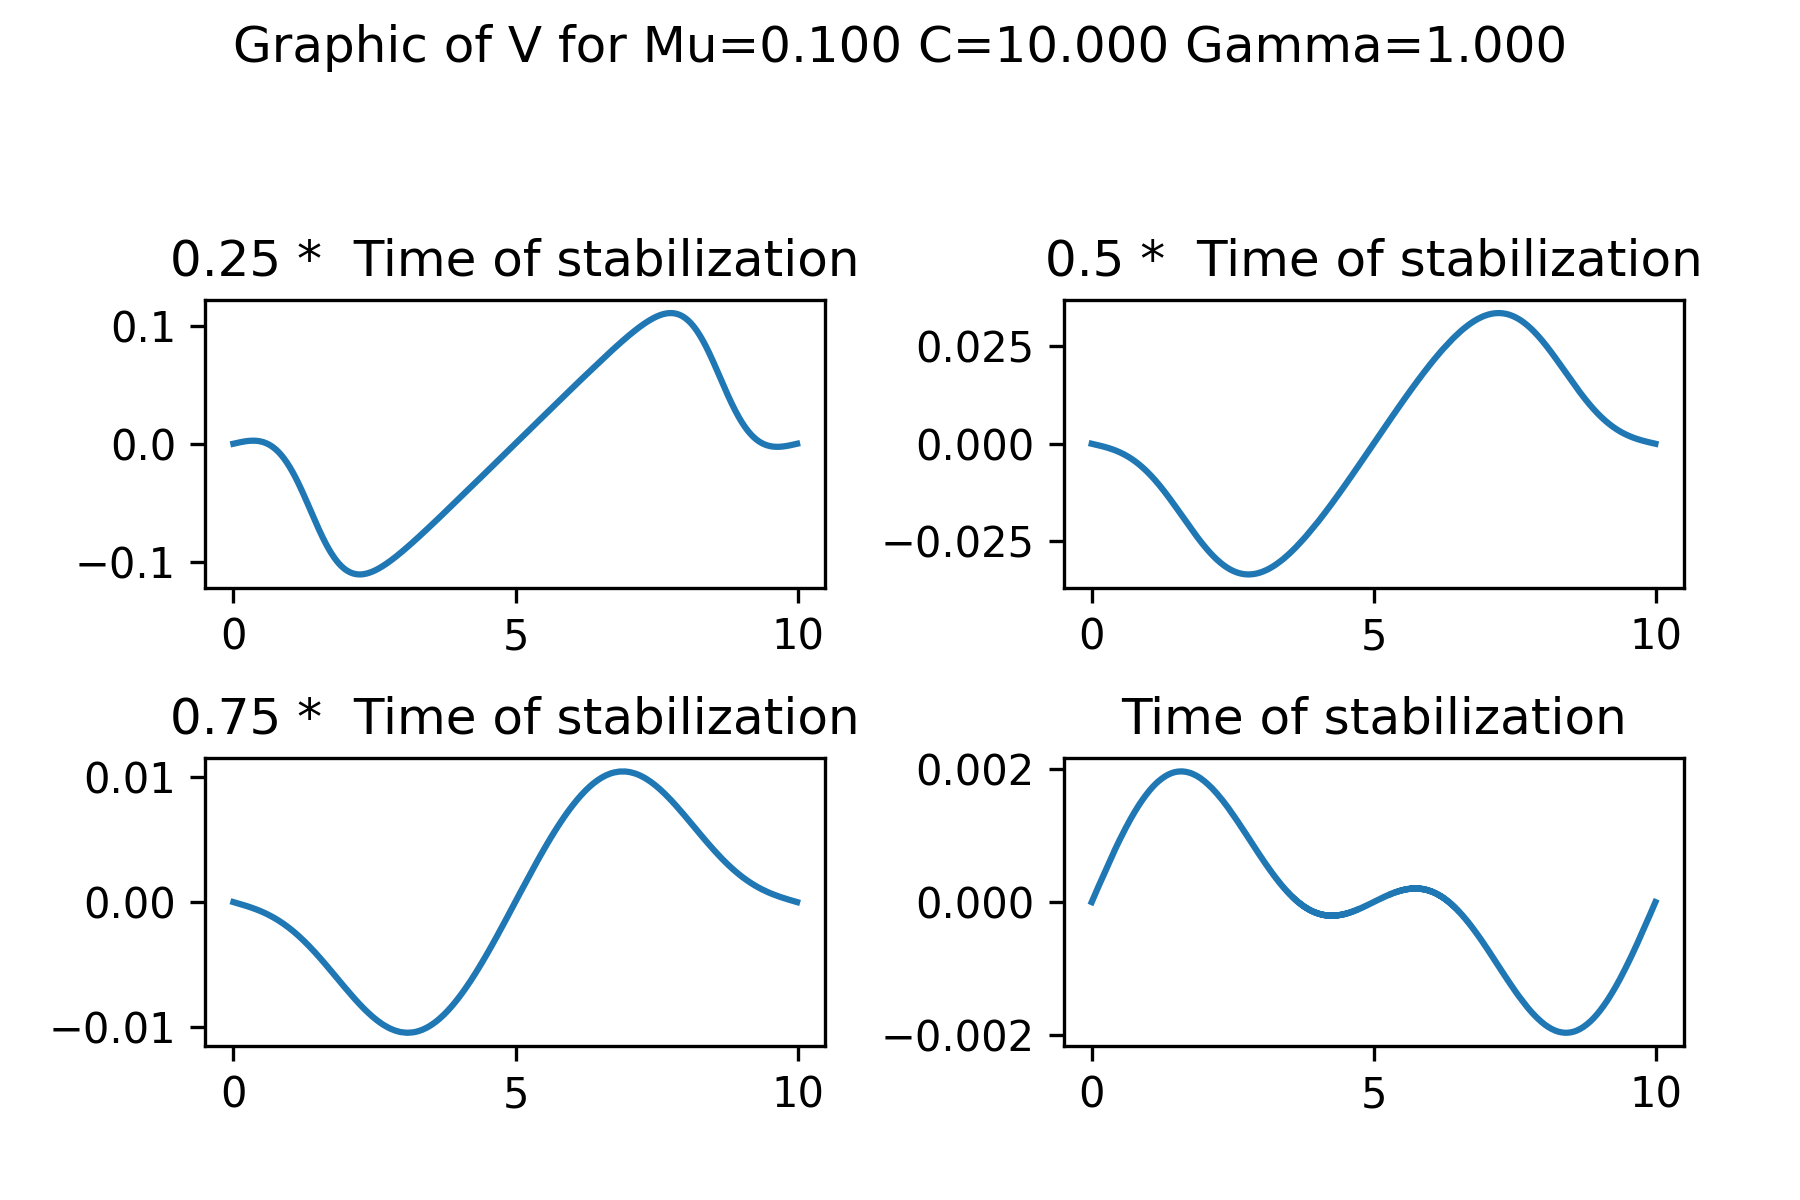
\includegraphics[scale=0.5]{../graphs_data_nonsmooth_1/slices/Graph_V_mu0.100_C10.000_gamma1.000.png}
\end{figure}

\begin{figure}[H]
	\centering
	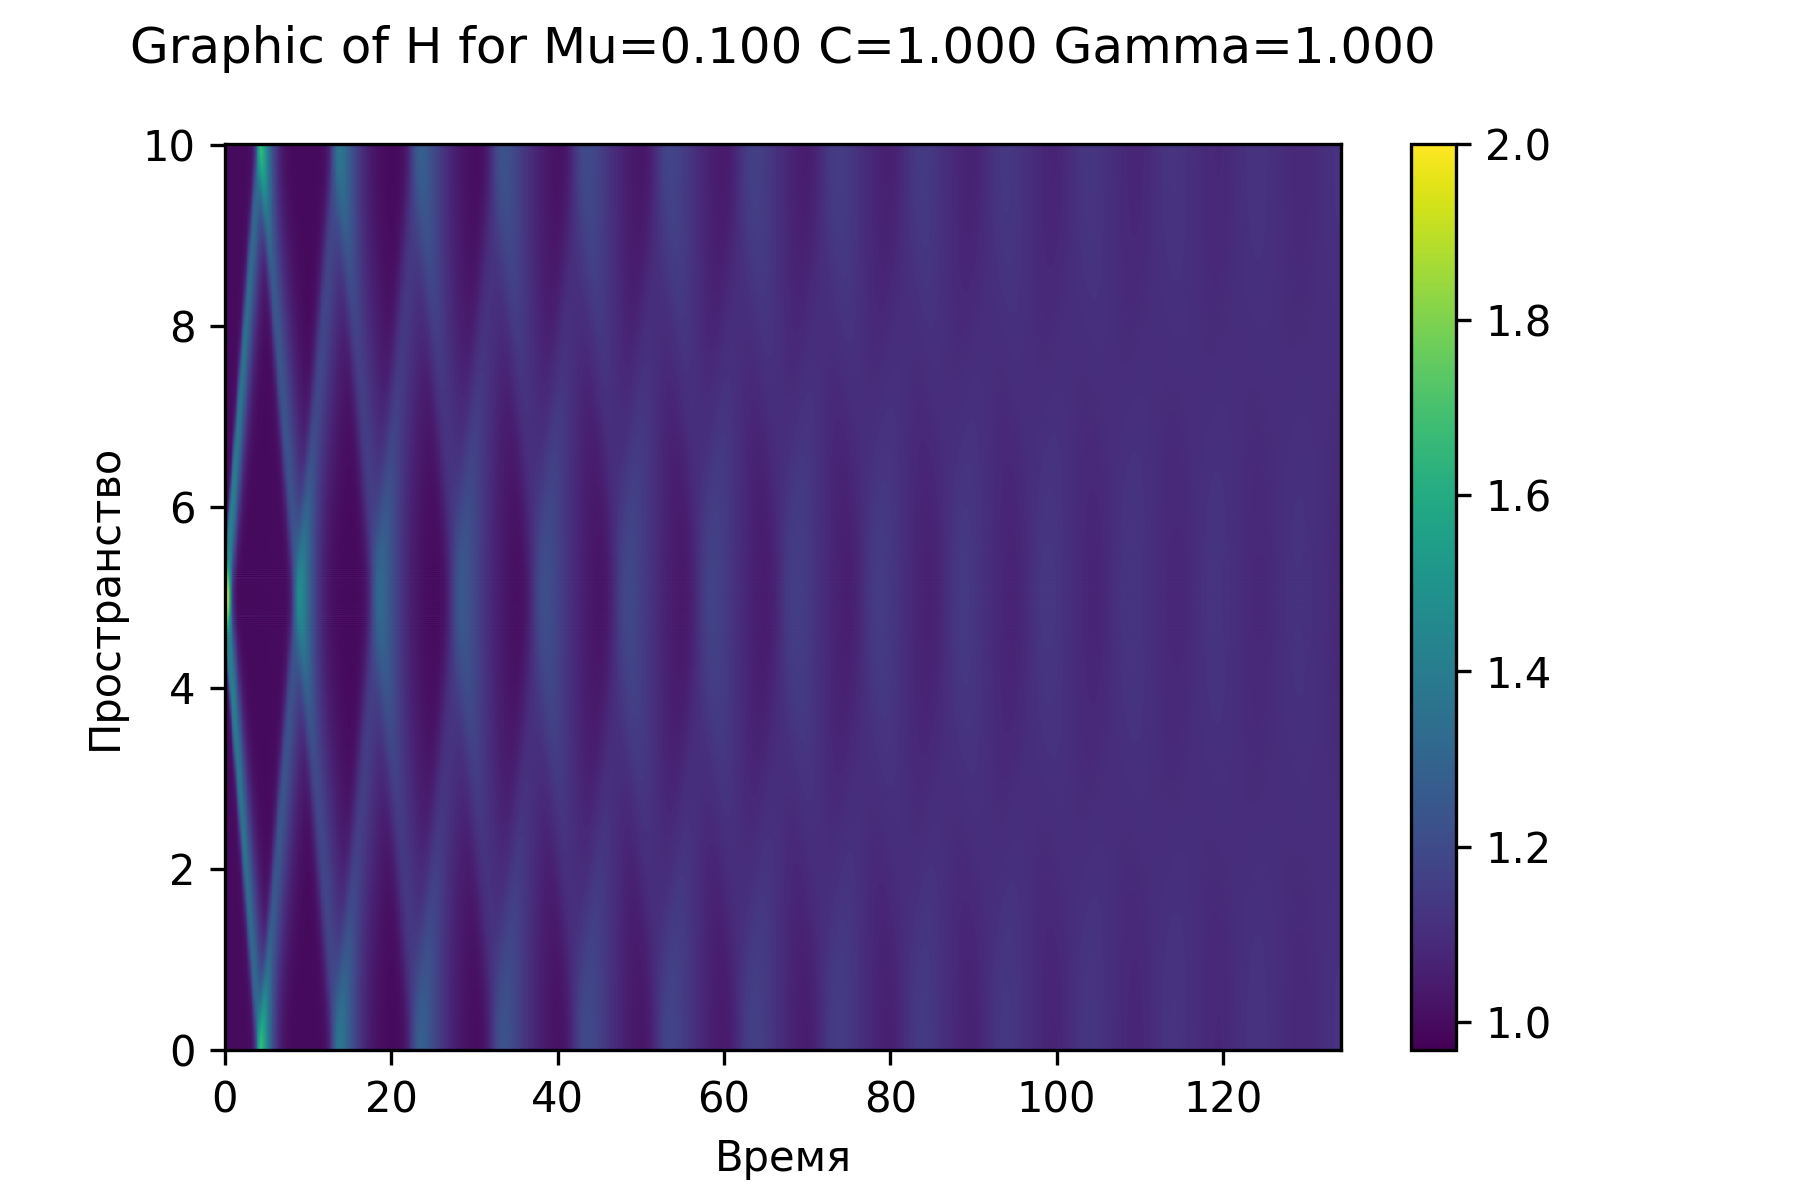
\includegraphics[scale=0.5]{../graphs_data_nonsmooth_1/value/Graph_H_mu0.100_C1.000_gamma1.000.png}
	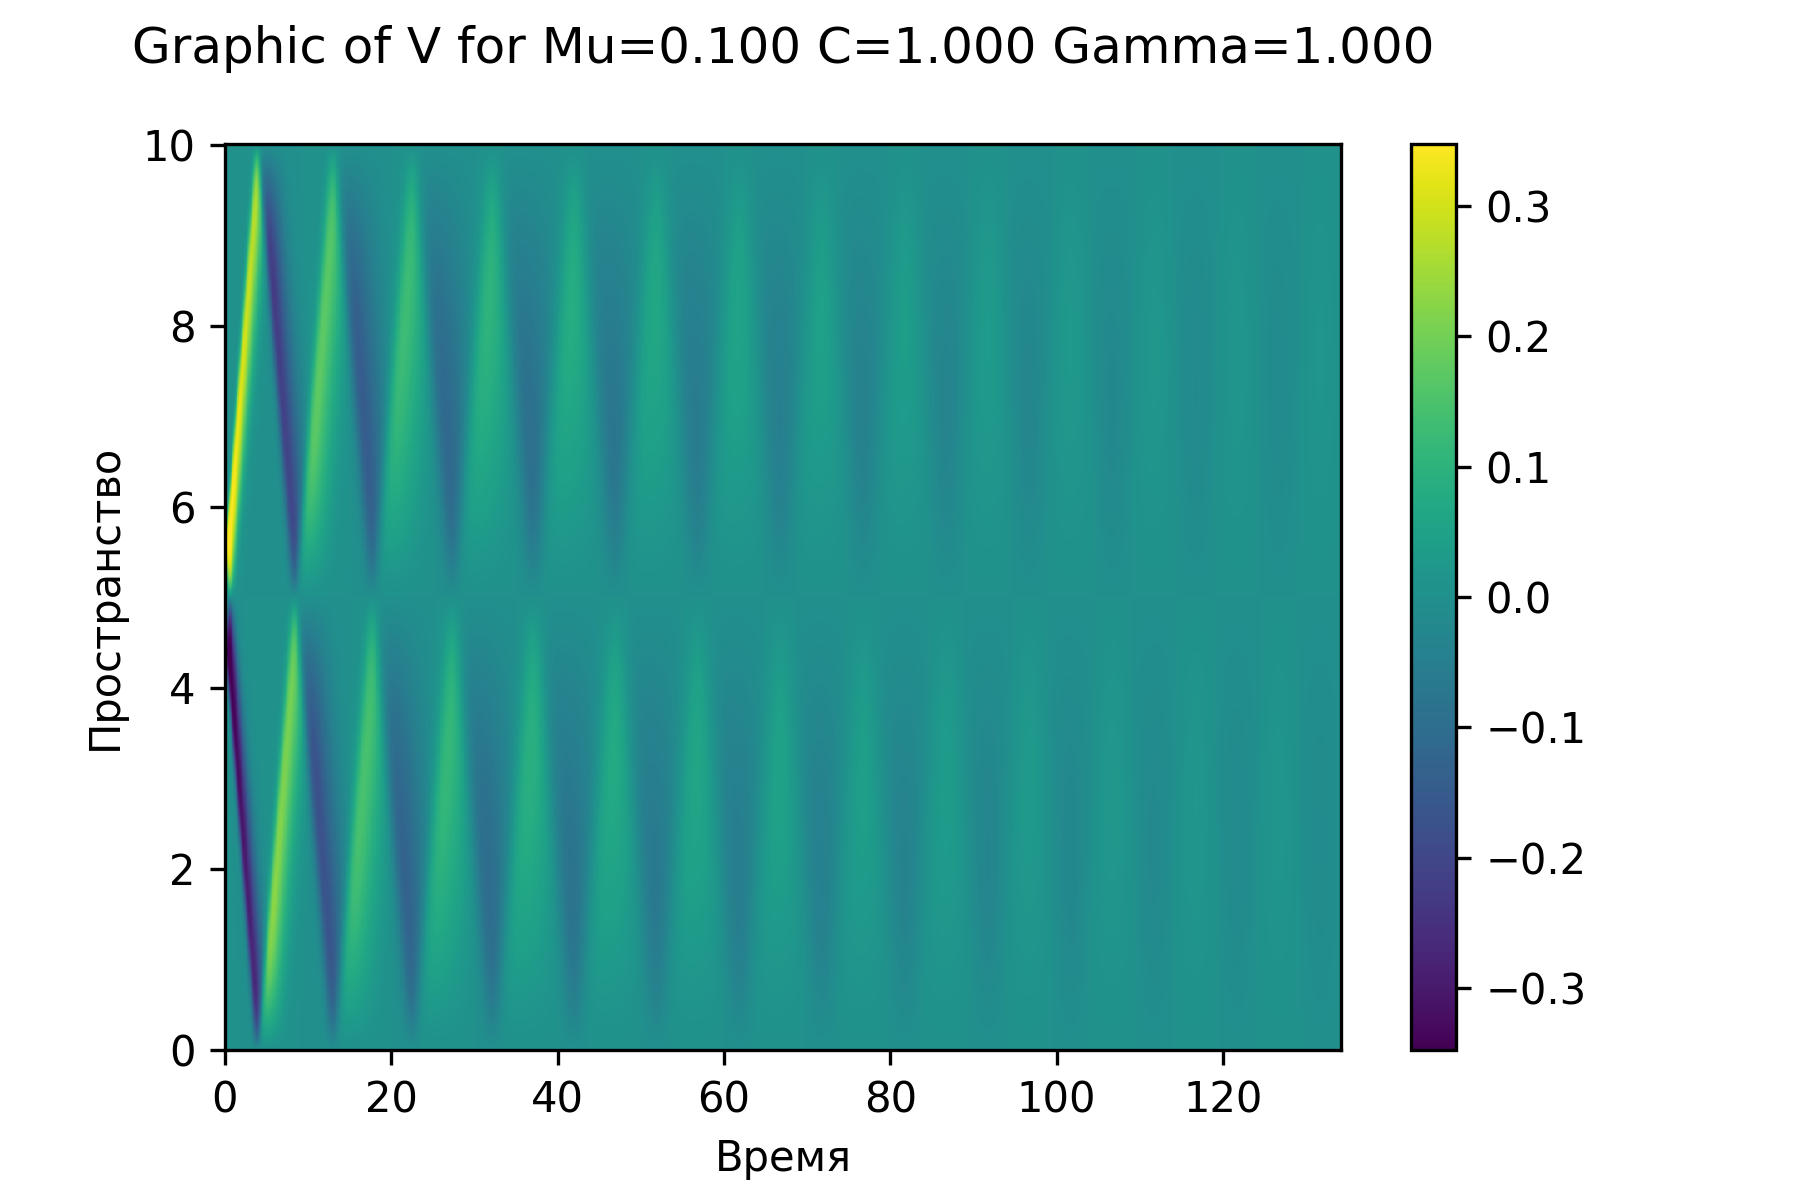
\includegraphics[scale=0.5]{../graphs_data_nonsmooth_1/value/Graph_V_mu0.100_C1.000_gamma1.000.png}	
	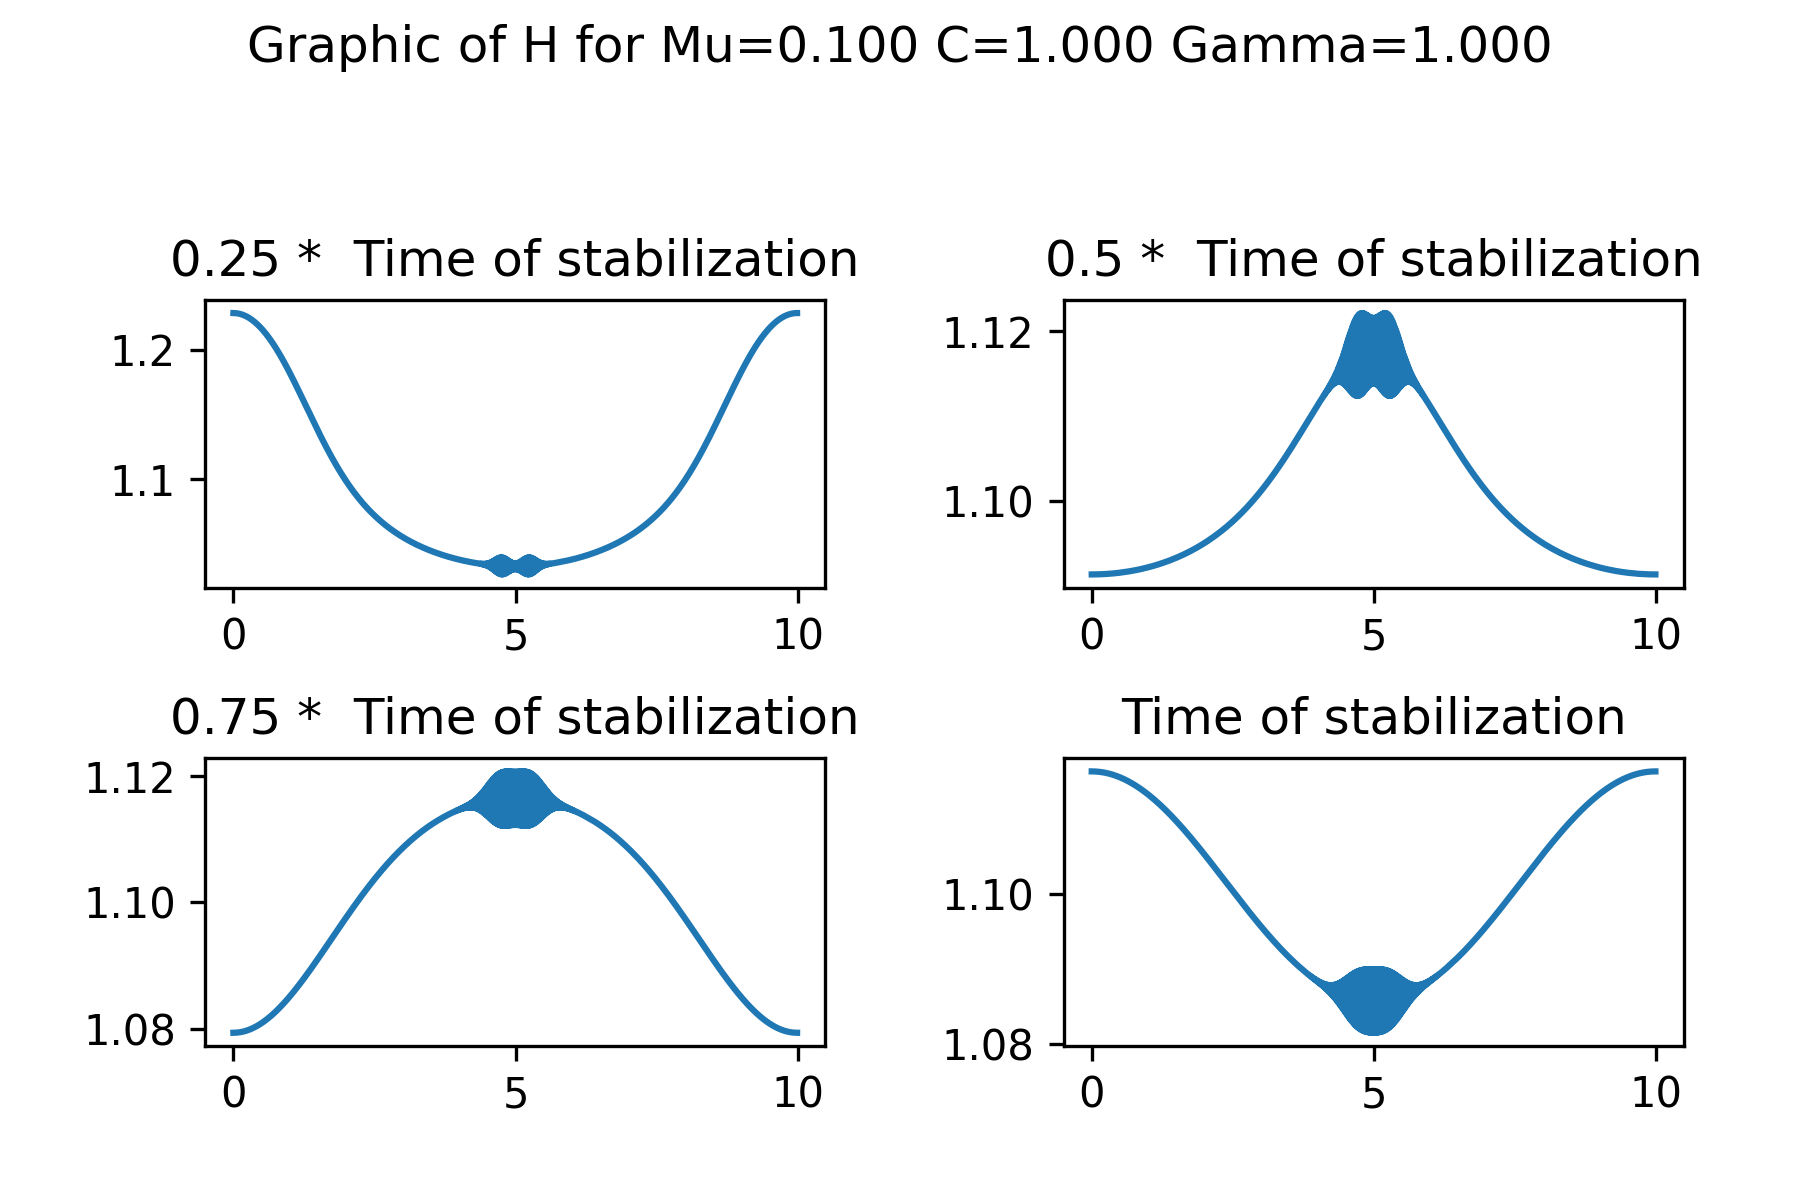
\includegraphics[scale=0.5]{../graphs_data_nonsmooth_1/slices/Graph_H_mu0.100_C1.000_gamma1.000.png}
	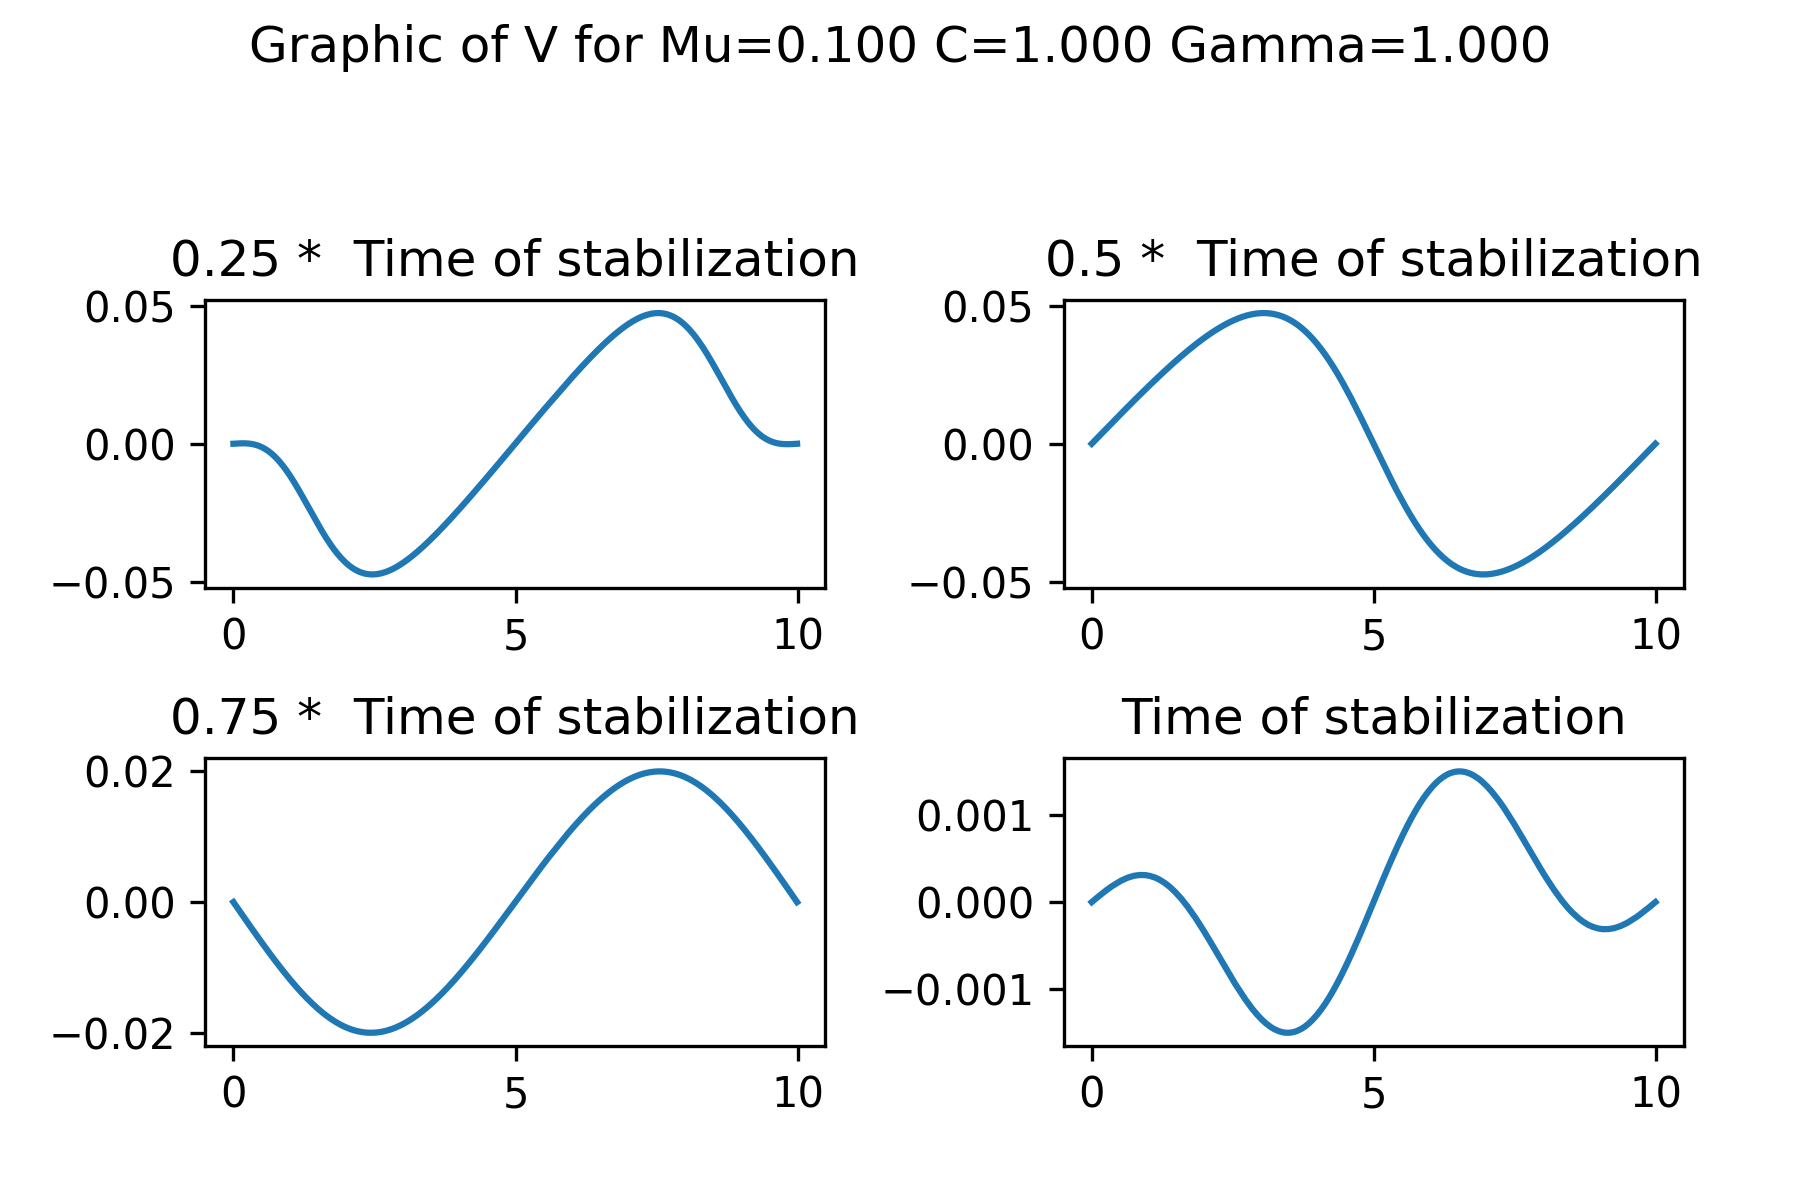
\includegraphics[scale=0.5]{../graphs_data_nonsmooth_1/slices/Graph_V_mu0.100_C1.000_gamma1.000.png}
\end{figure}

\begin{figure}[H]
	\centering
	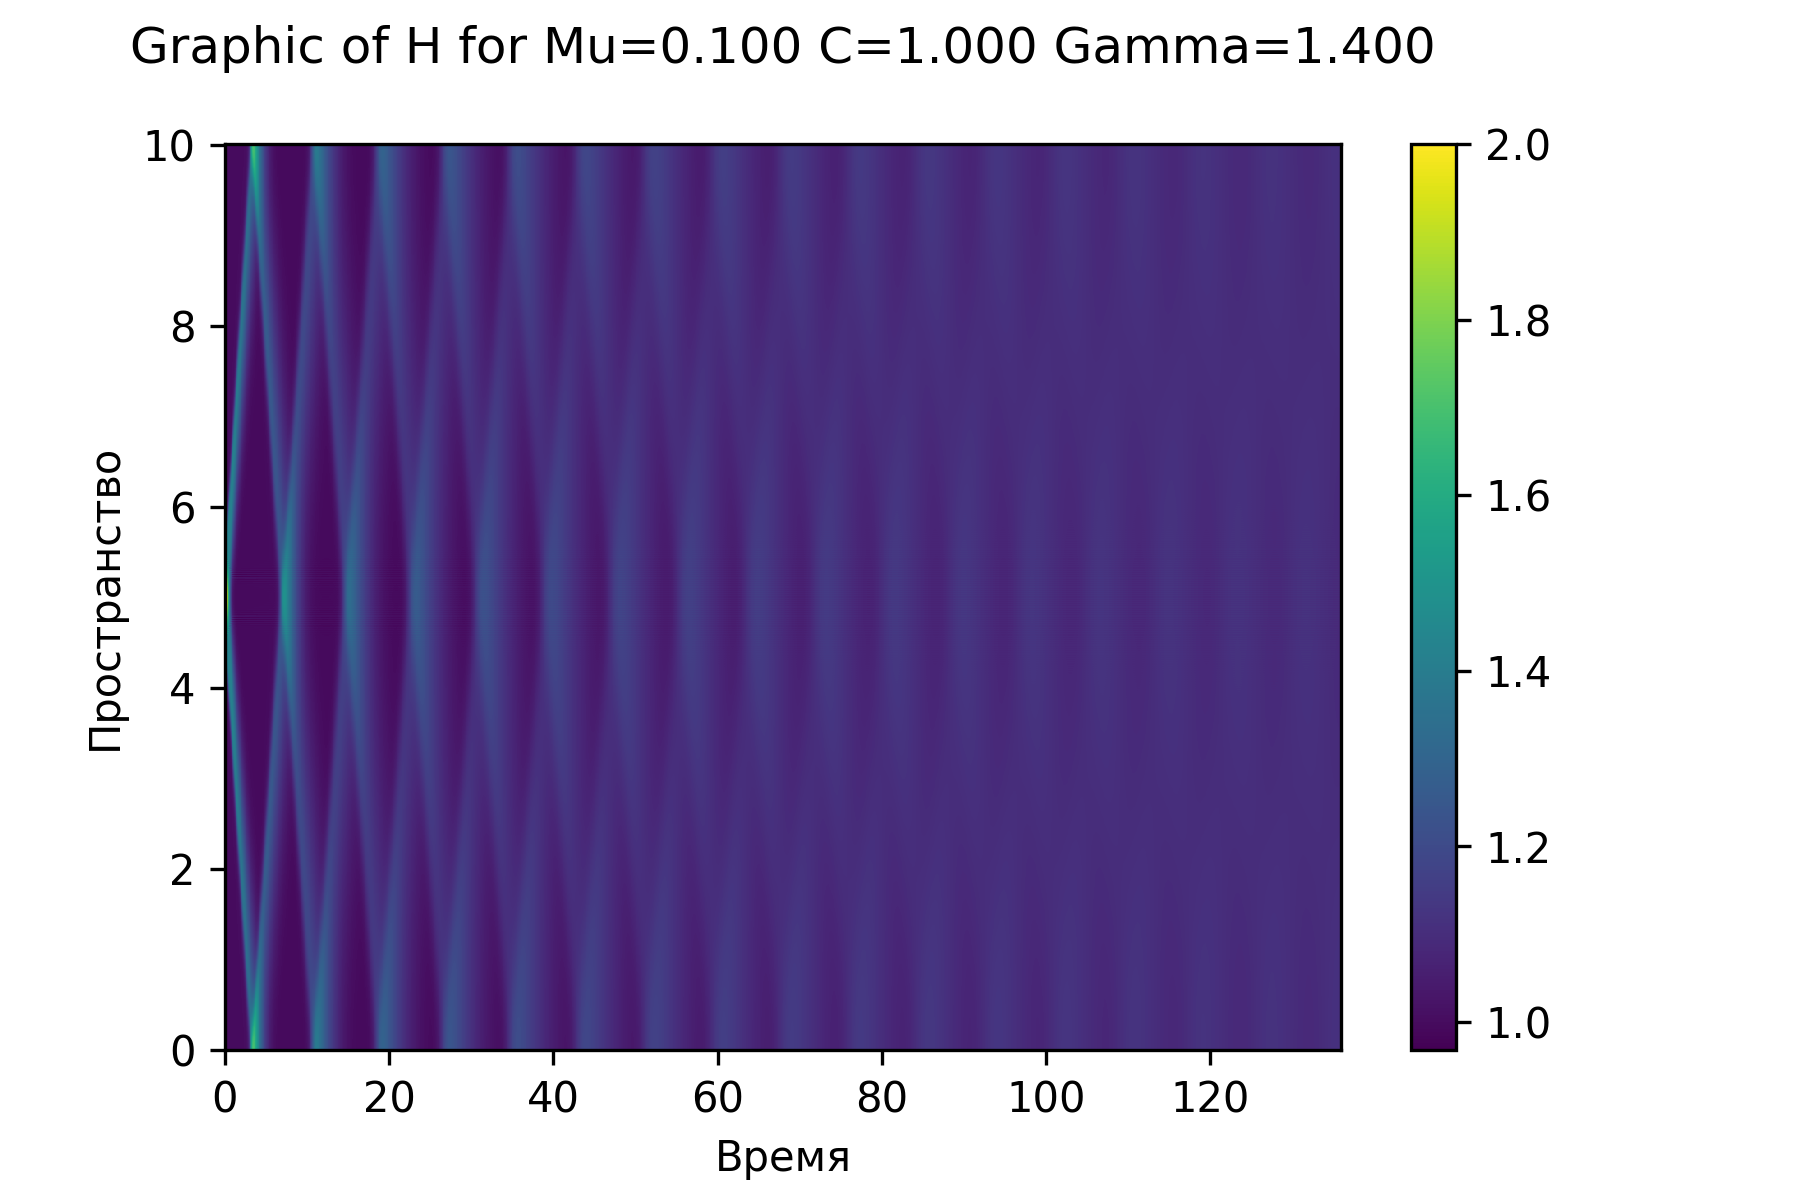
\includegraphics[scale=0.5]{../graphs_data_nonsmooth_1/value/Graph_H_mu0.100_C1.000_gamma1.400.png}
	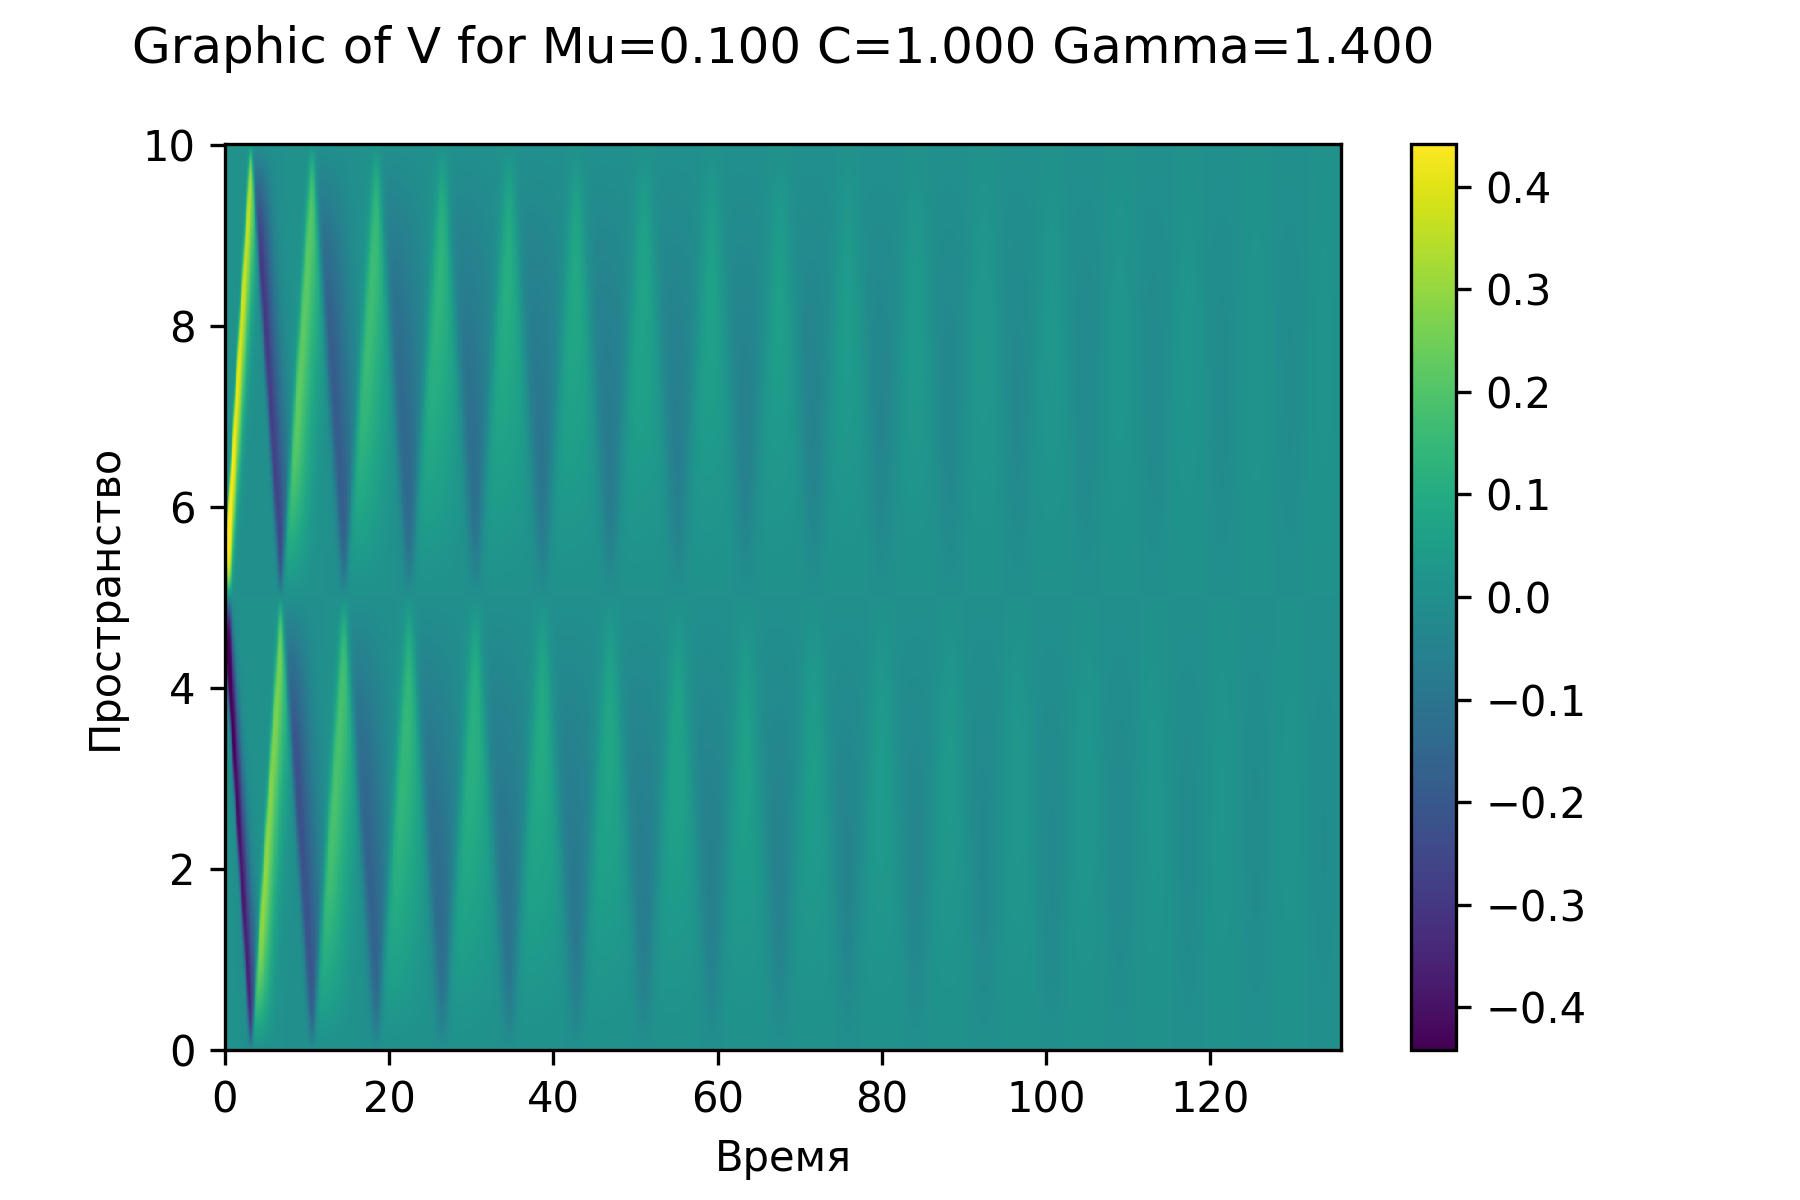
\includegraphics[scale=0.5]{../graphs_data_nonsmooth_1/value/Graph_V_mu0.100_C1.000_gamma1.400.png}	
	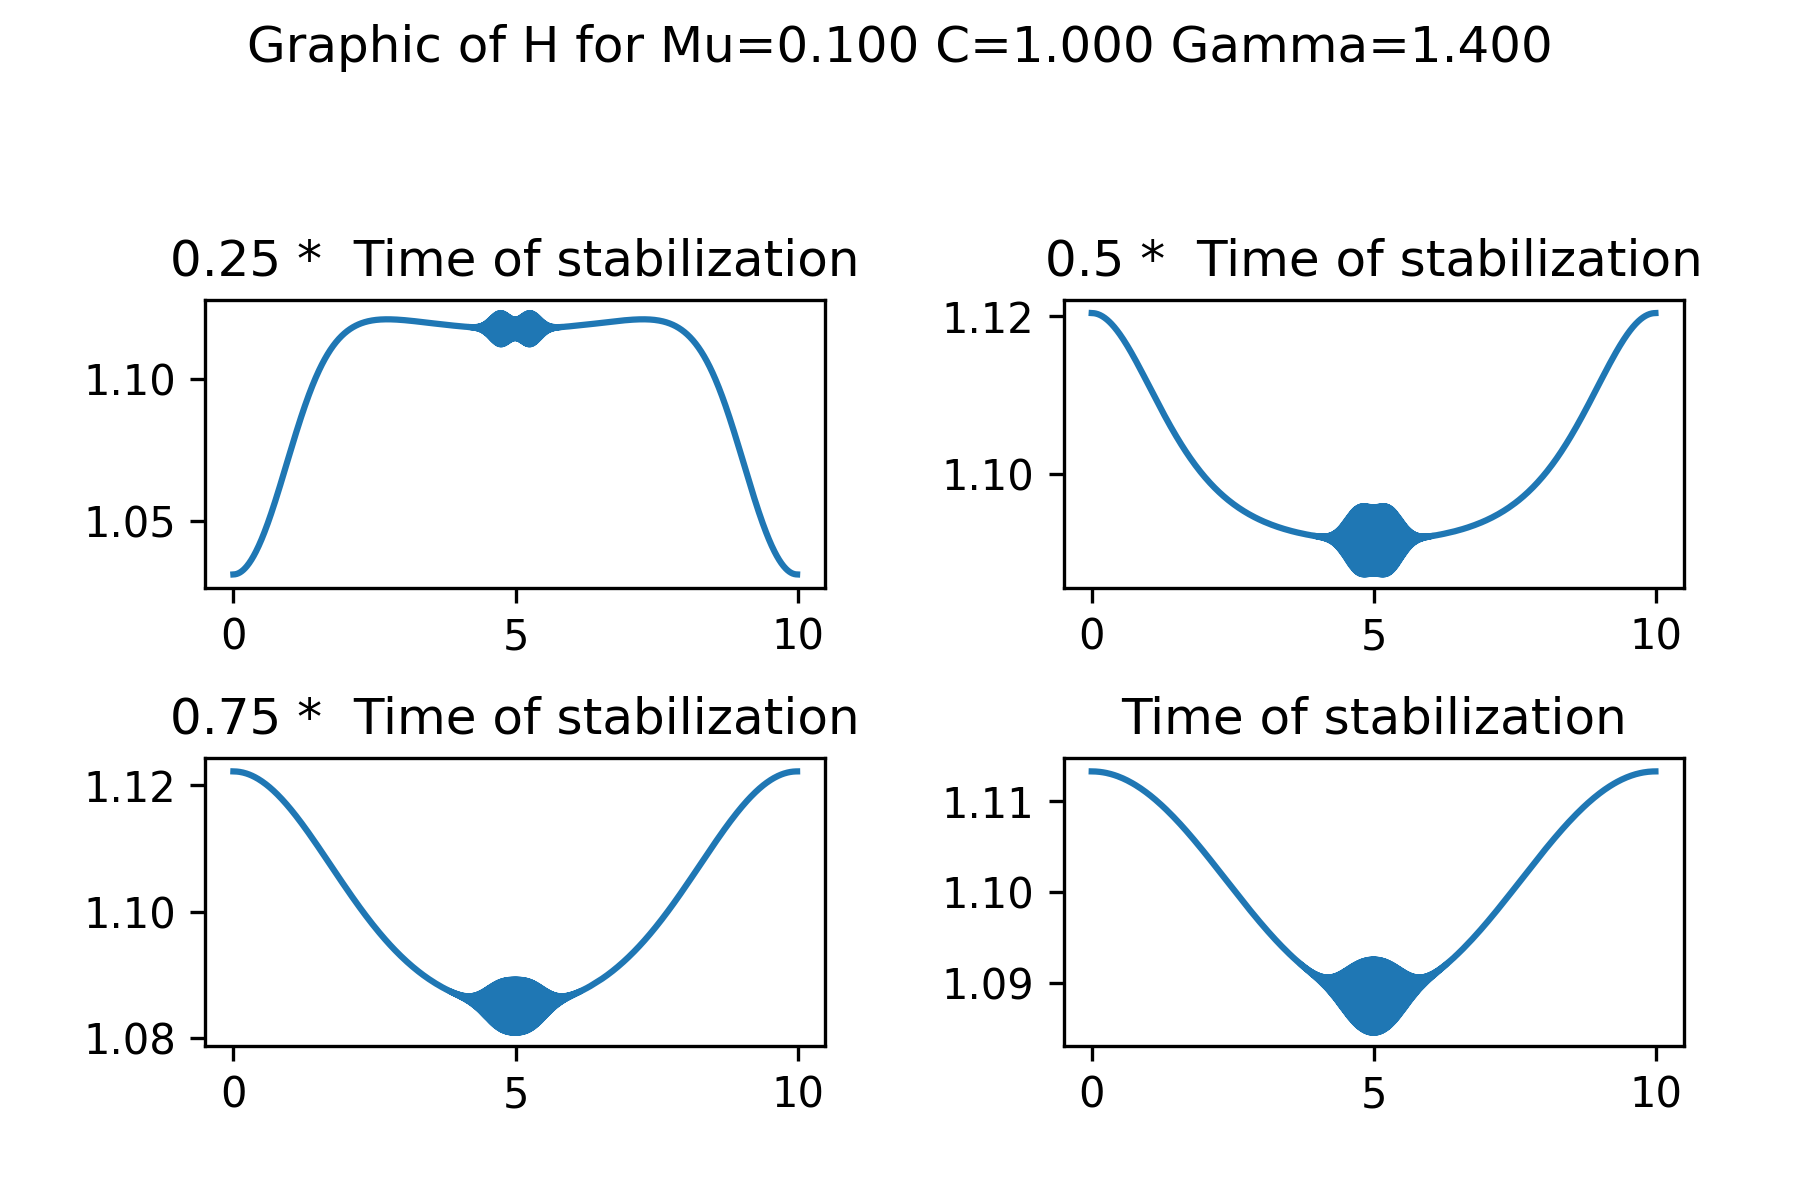
\includegraphics[scale=0.5]{../graphs_data_nonsmooth_1/slices/Graph_H_mu0.100_C1.000_gamma1.400.png}
	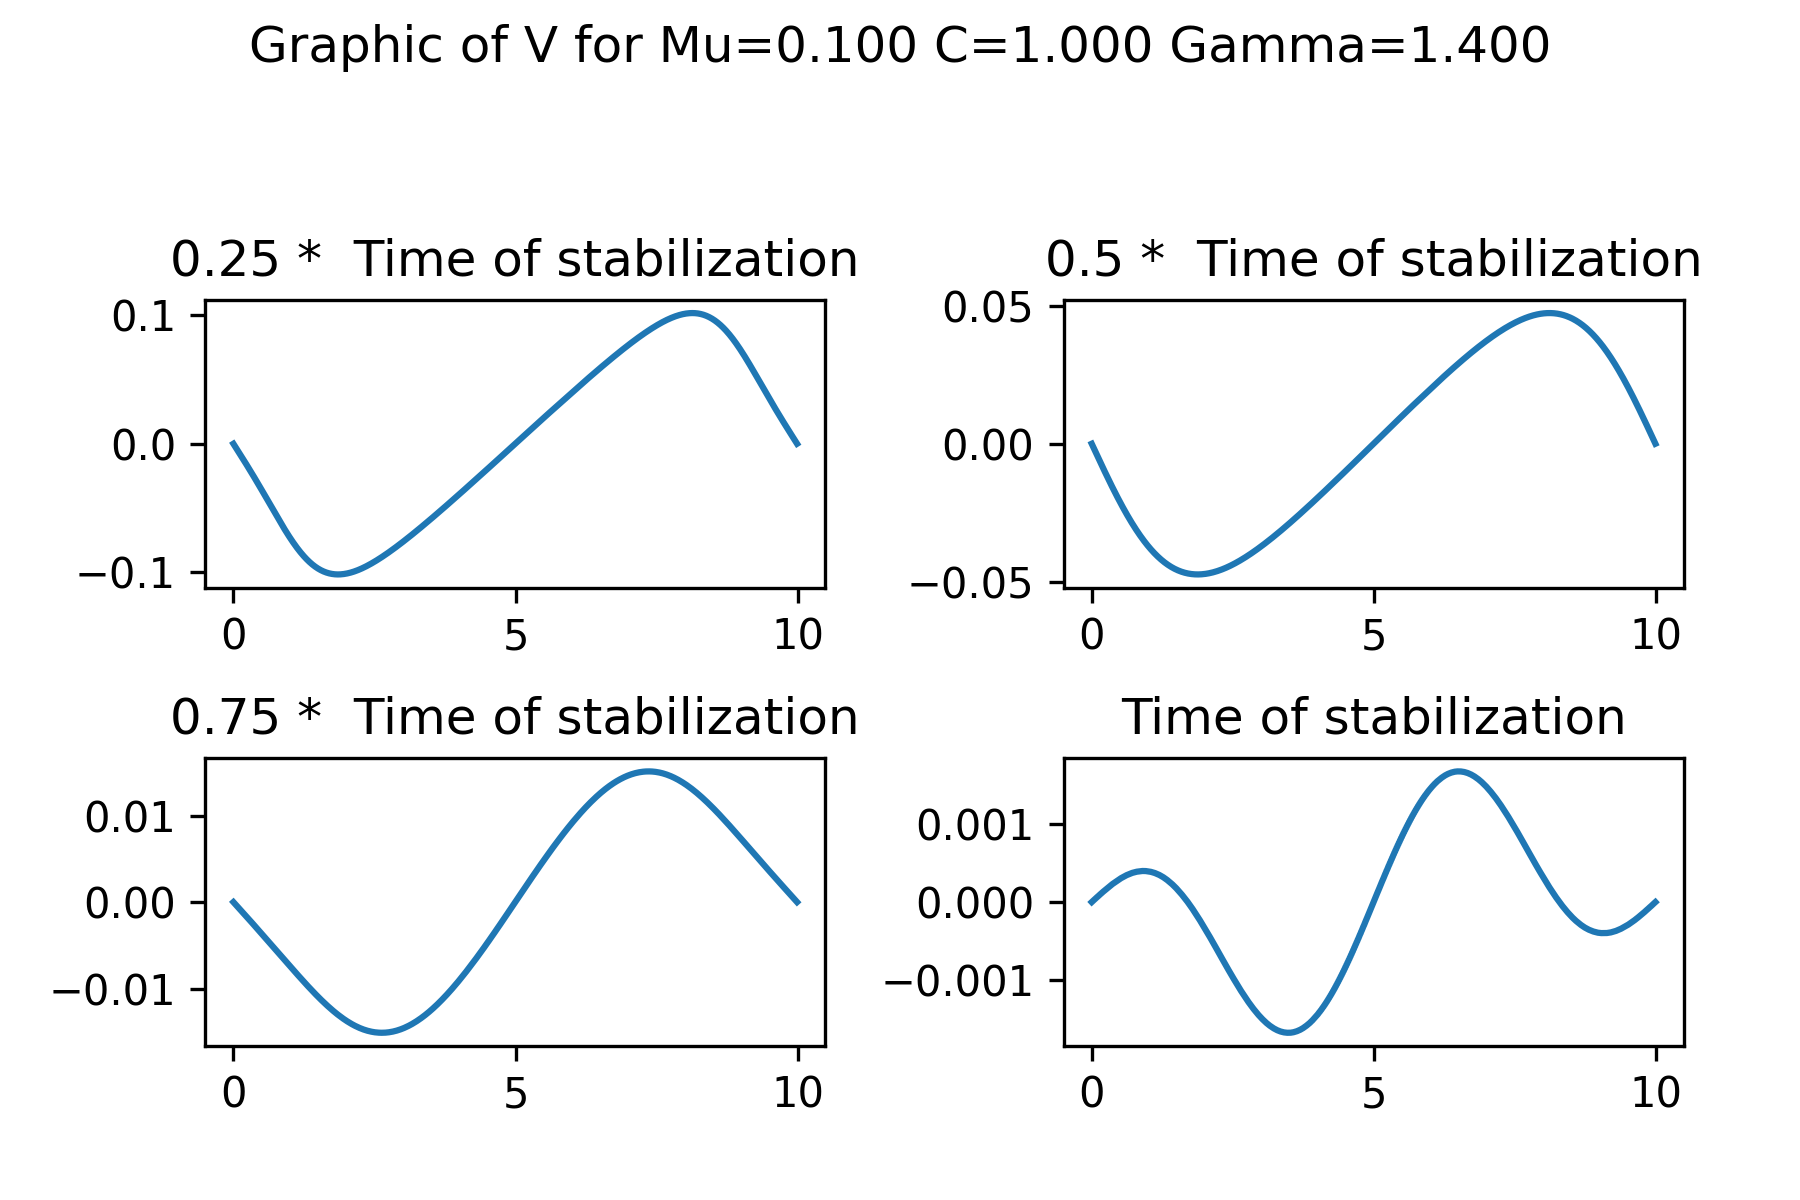
\includegraphics[scale=0.5]{../graphs_data_nonsmooth_1/slices/Graph_V_mu0.100_C1.000_gamma1.400.png}
\end{figure}

Период колебаний не зависит от $\mu$, однако при увеличении $C$ и $\gamma$ частота колебаний увеличивается. Однако при уменьшении $\mu$ увеличивается время стабилизации процесса.


\newpage
Приведем также графики норм для различных начальных параметров.
\begin{figure}[H]
	\centering
	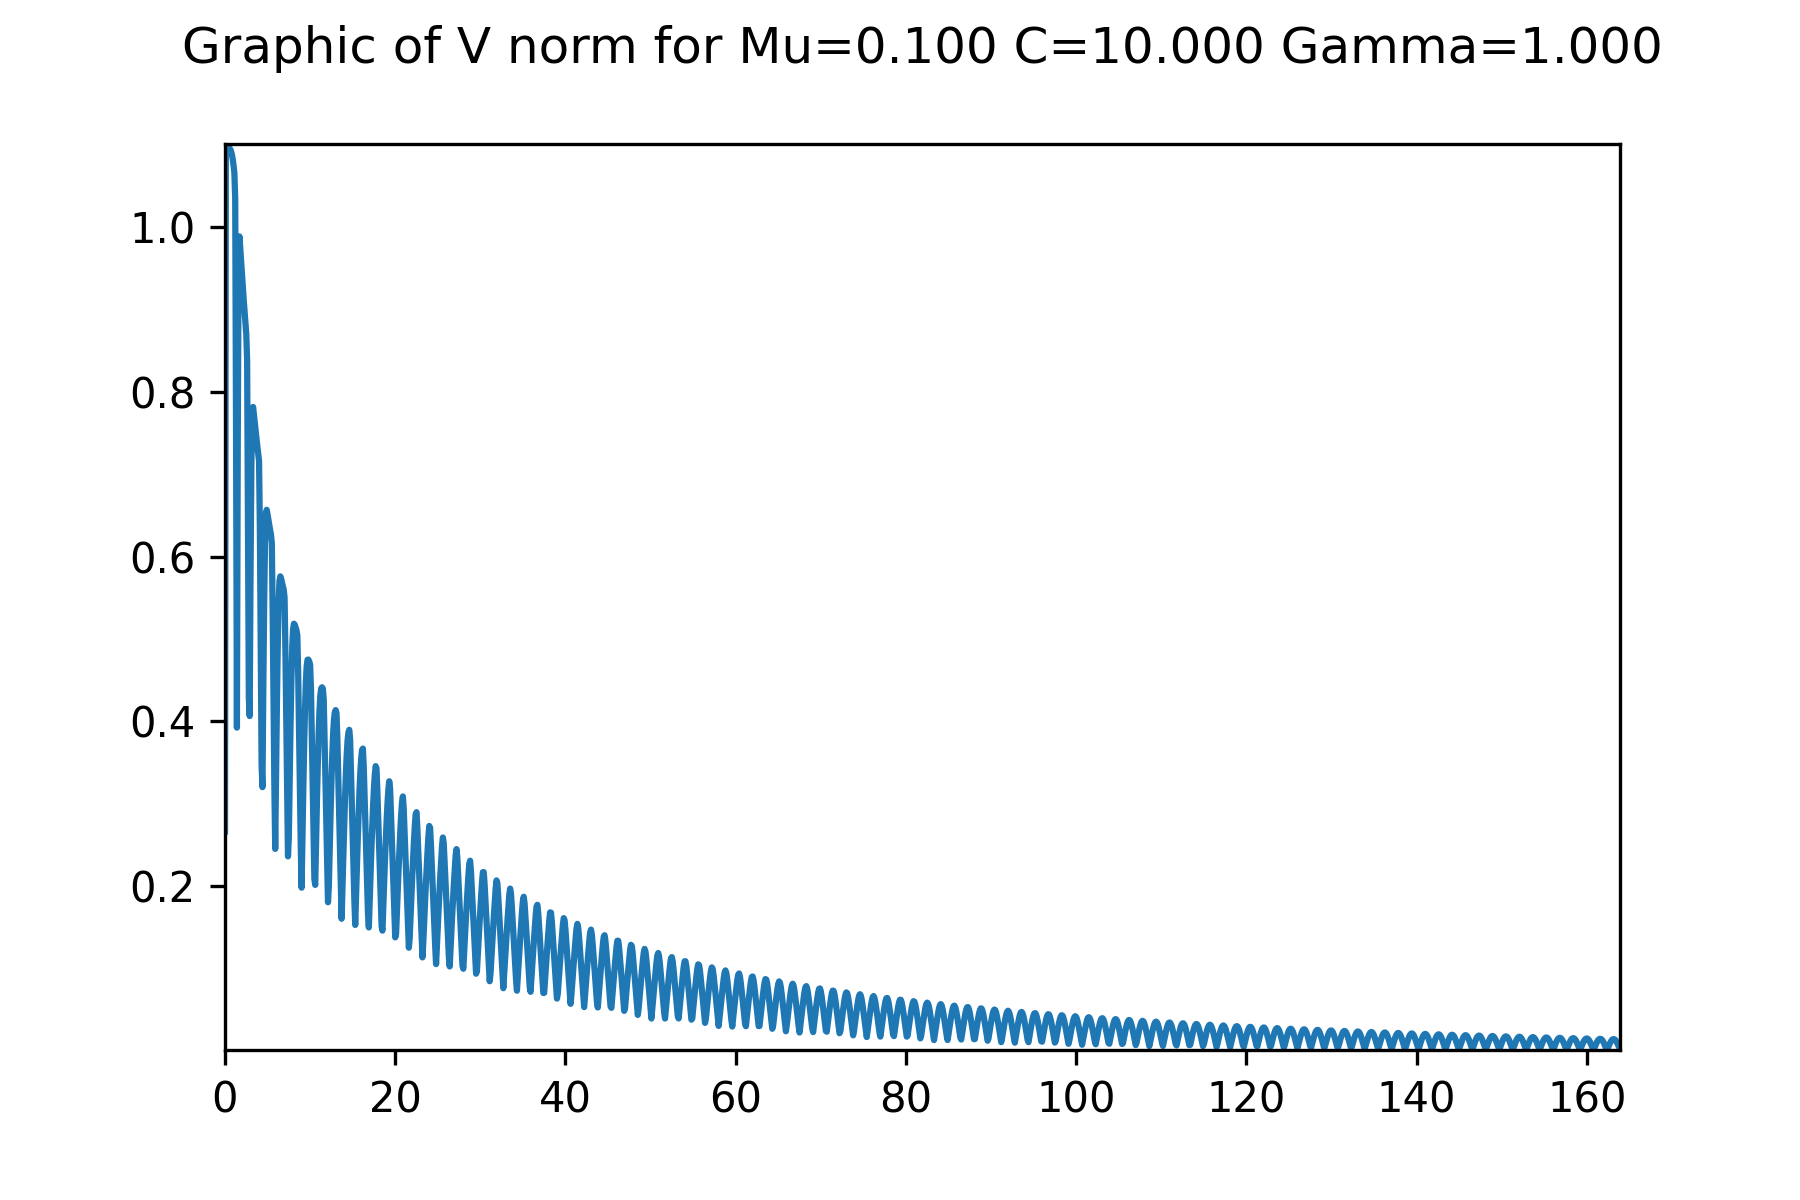
\includegraphics[scale=0.65]{../graphs_data_nonsmooth_1/norms/Graph_V_norms_mu0.100_C10.000_gamma1.000.png}
	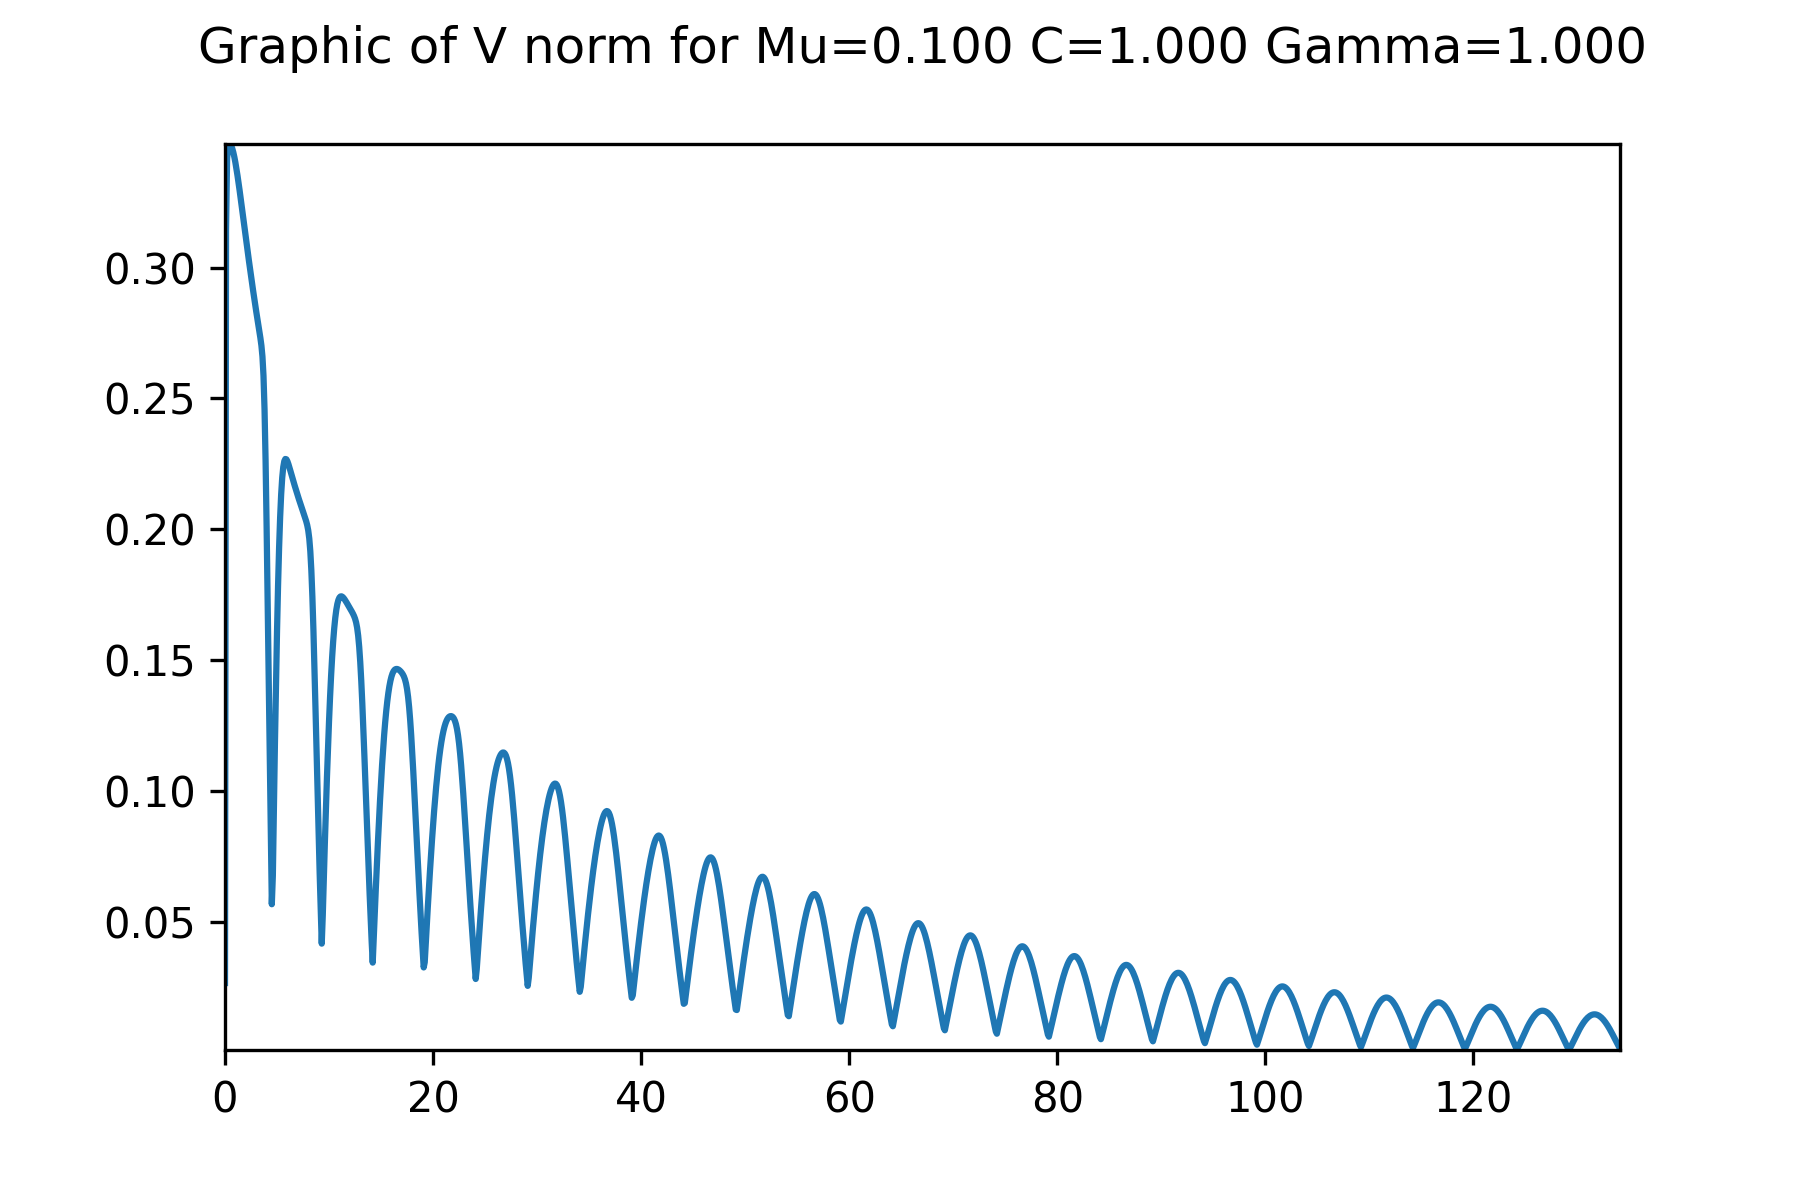
\includegraphics[scale=0.65]{../graphs_data_nonsmooth_1/norms/Graph_V_norms_mu0.100_C1.000_gamma1.000.png}	
	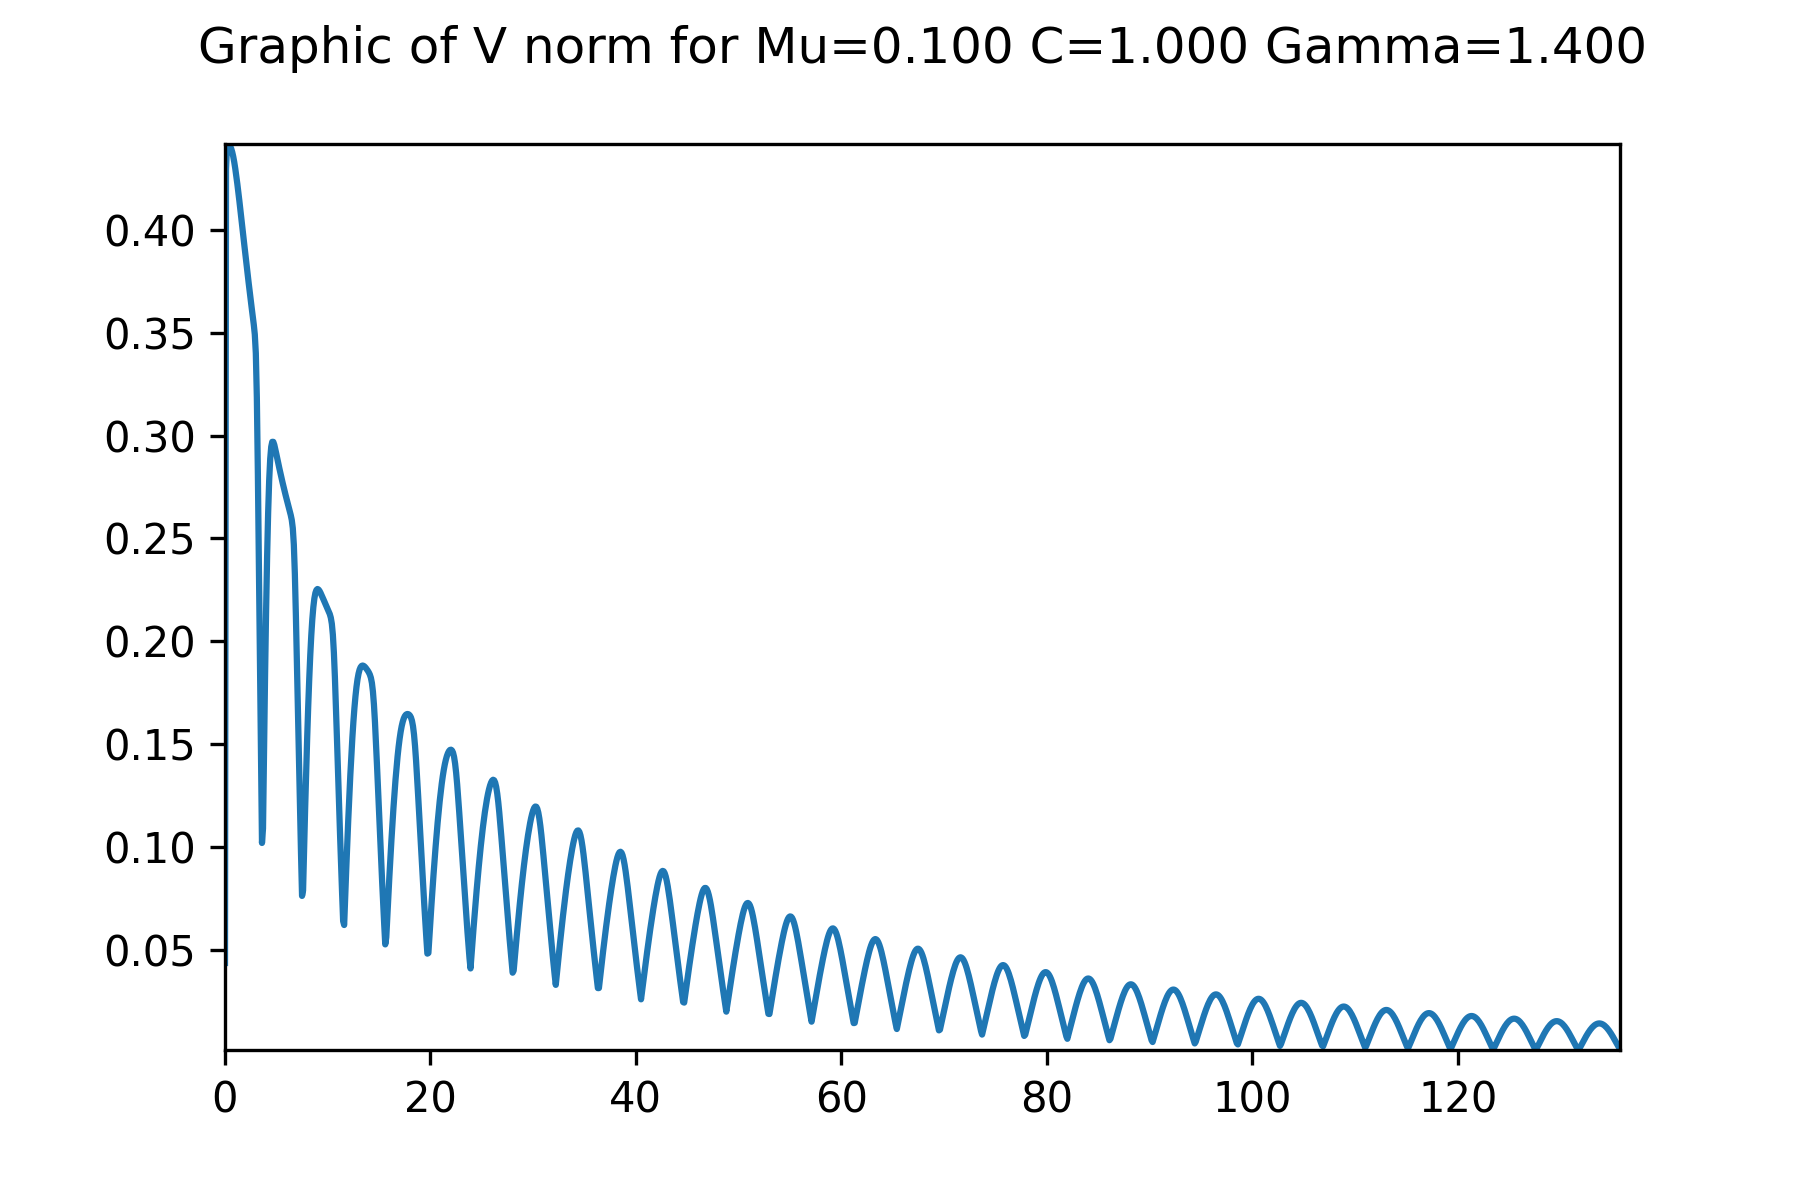
\includegraphics[scale=0.65]{../graphs_data_nonsmooth_1/norms/Graph_V_norms_mu0.100_C1.000_gamma1.400.png}
\end{figure}


\begin{figure}[H]
	\centering
	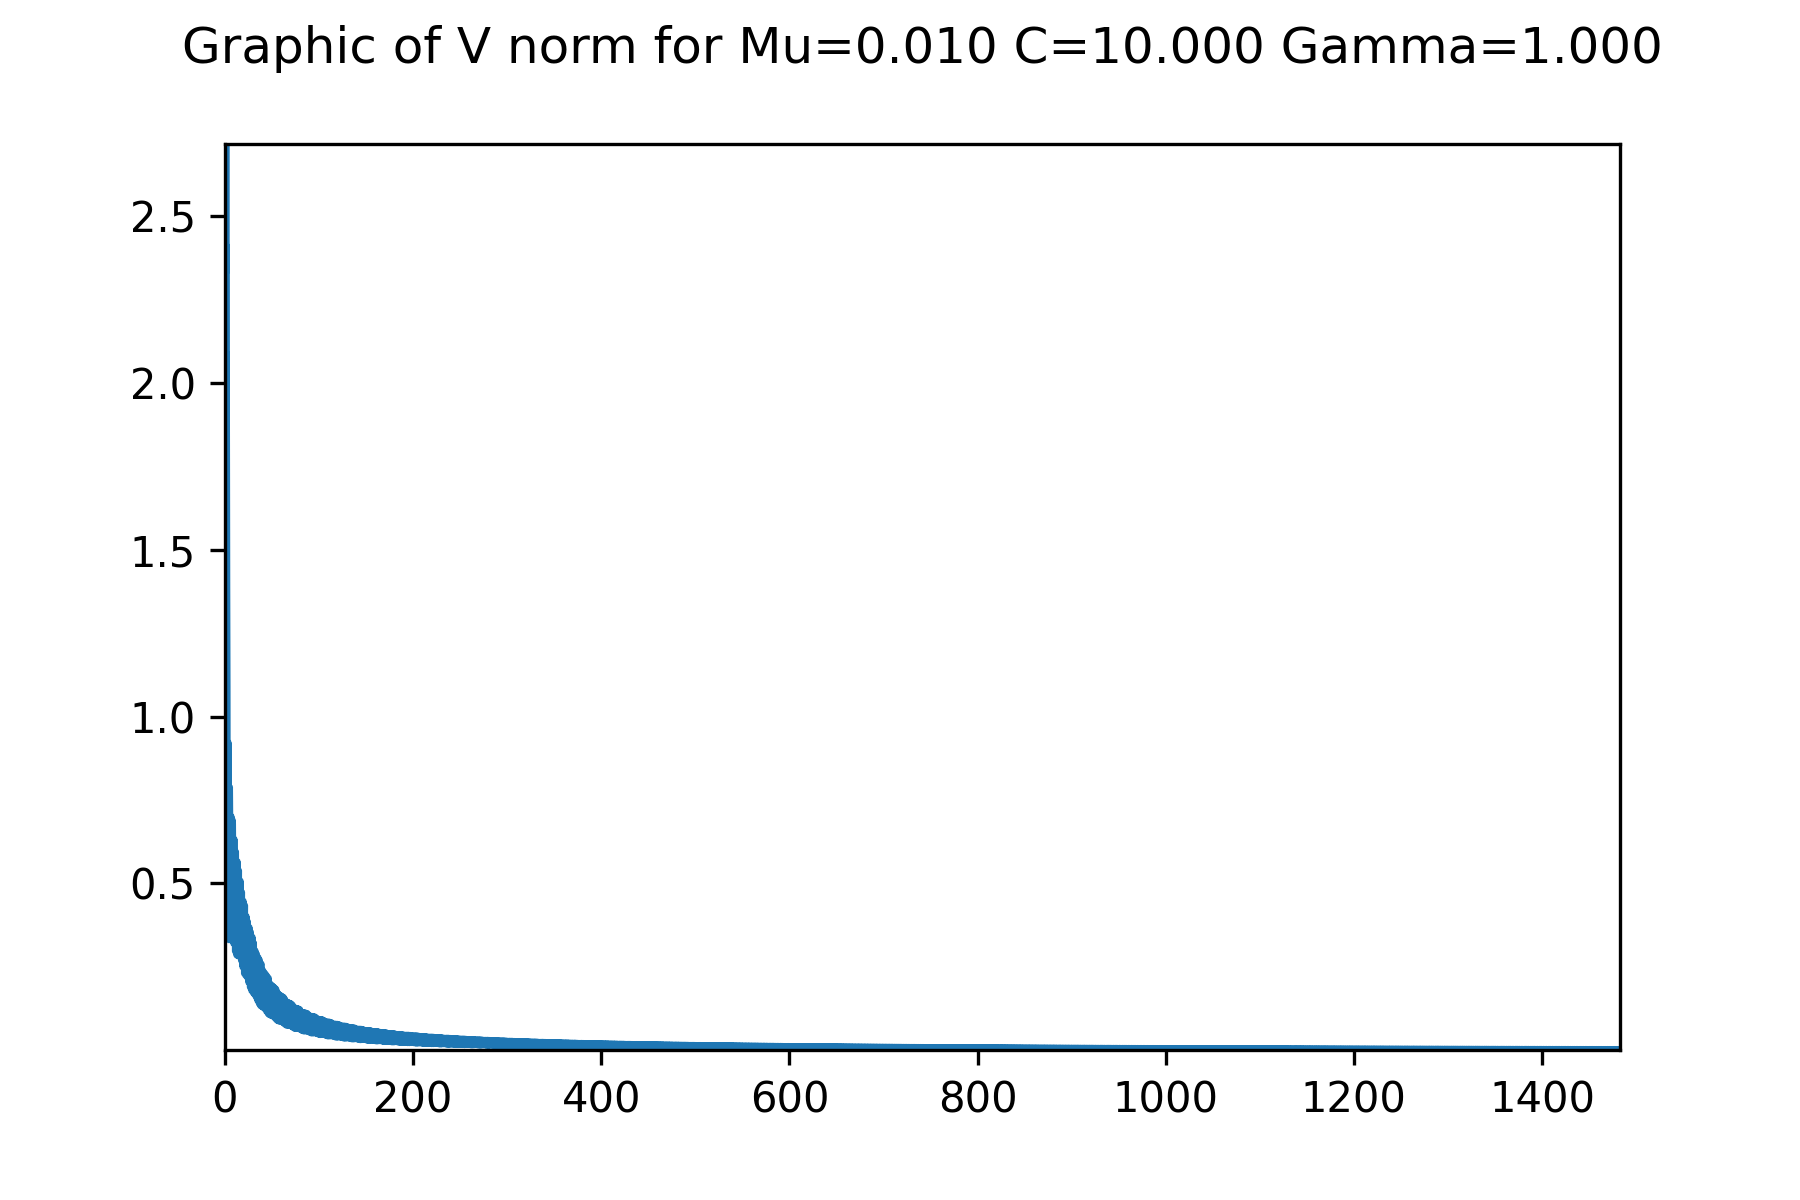
\includegraphics[scale=0.65]{../graphs_data_nonsmooth_1/norms/Graph_V_norms_mu0.010_C10.000_gamma1.000.png}
	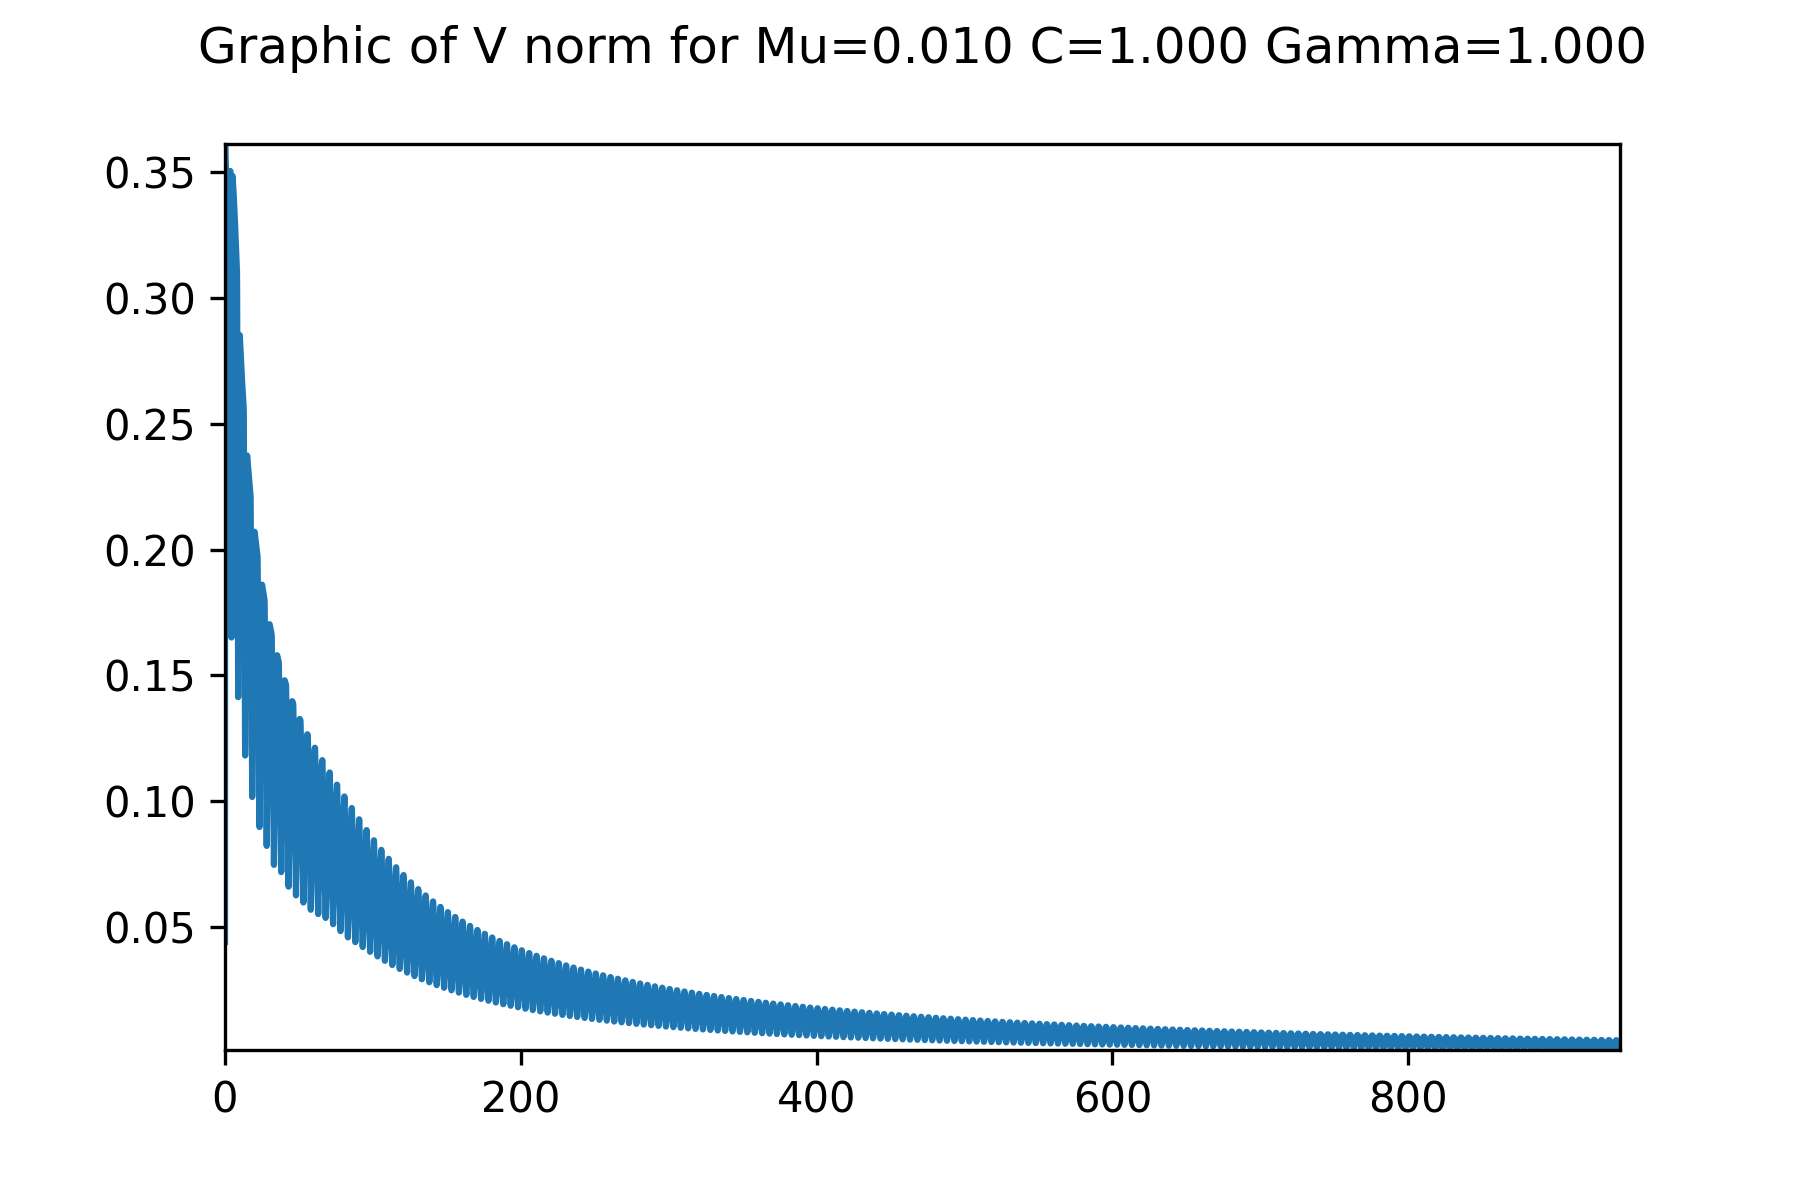
\includegraphics[scale=0.65]{../graphs_data_nonsmooth_1/norms/Graph_V_norms_mu0.010_C1.000_gamma1.000.png}	
	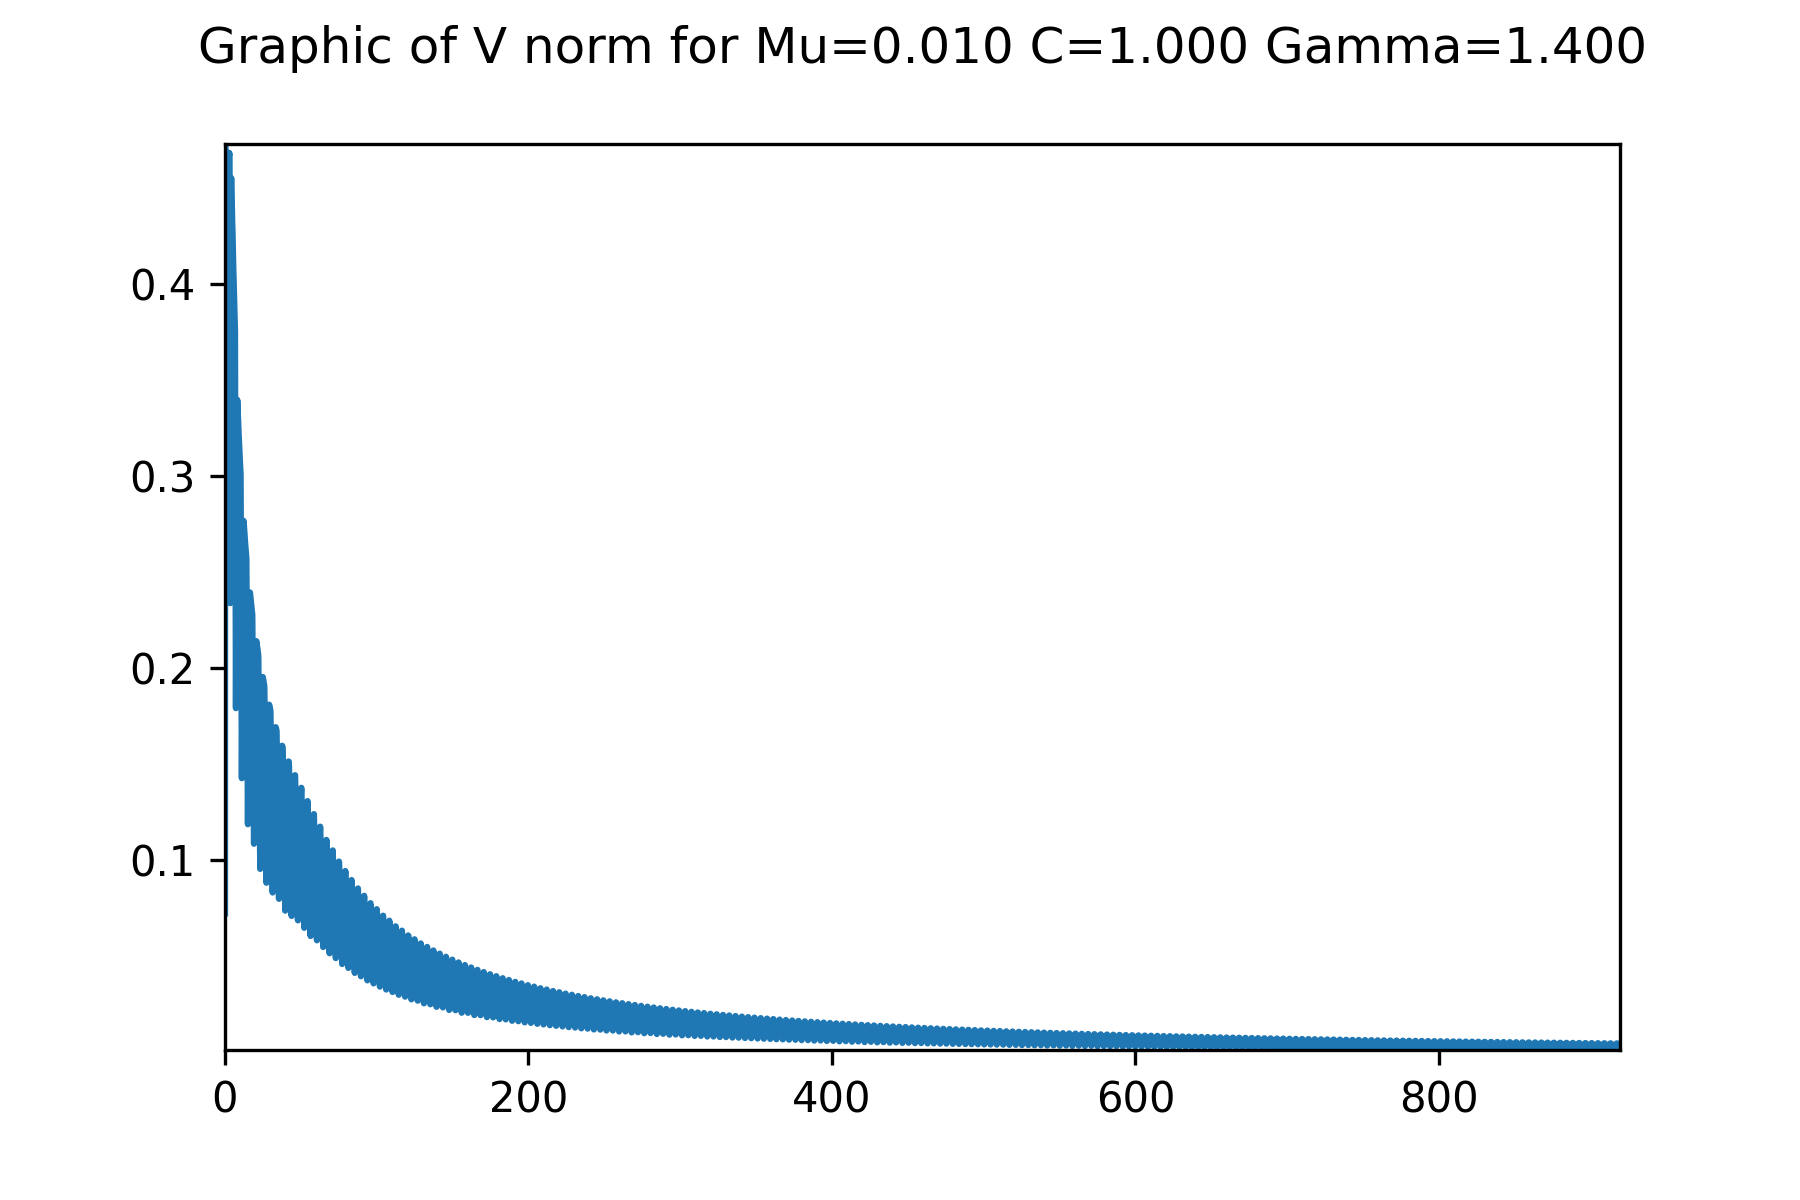
\includegraphics[scale=0.65]{../graphs_data_nonsmooth_1/norms/Graph_V_norms_mu0.010_C1.000_gamma1.400.png}
\end{figure}

\newpage
Далее приведены значения $\Delta m(n)$ на измельченных и обычных сетках. А также их графическое представление.

\begin{center}
Table of mass loss. $\mu = 0.1000$ \, $C = 10.0000$, $\gamma = 1.0000$
  
\begin{tabular}{|p{0.8in}|p{0.8in}|p{0.8in}|p{0.8in}|p{0.8in}|p{0.8in}|p{0.8in}|} \hline
$K$ &$N_0$ &$N_0 \tau$ &$n = \frac{N_0}{4}$ &$n = \frac{N_0}{2}$ &$n = \frac{3N_0}{4}$ &$n = N_0$ \\ \hline 
0 &444220 &4.442e+02 &2.725e-04 &2.826e-04 &2.854e-04 &2.863e-04 \\ \hline 
1 &888439 &4.442e+02 &1.288e-04 &1.336e-04 &1.349e-04 &1.353e-04 \\ \hline 
2 &1776877 &4.442e+02 &6.272e-05 &6.505e-05 &6.568e-05 &6.586e-05 \\ \hline 
3 &3553753 &4.442e+02 &3.096e-05 &3.211e-05 &3.242e-05 &3.251e-05 \\ \hline 

\end{tabular}\\[20pt]
\end{center}

\begin{center}
Table of mass loss. $\mu = 0.1000$ \, $C = 1.0000$, $\gamma = 1.0000$
  
\begin{tabular}{|p{0.8in}|p{0.8in}|p{0.8in}|p{0.8in}|p{0.8in}|p{0.8in}|p{0.8in}|} \hline
$K$ &$N_0$ &$N_0 \tau$ &$n = \frac{N_0}{4}$ &$n = \frac{N_0}{2}$ &$n = \frac{3N_0}{4}$ &$n = N_0$ \\ \hline 
0 &414339 &4.143e+02 &2.568e-04 &2.822e-04 &2.735e-04 &2.757e-04 \\ \hline 
1 &828677 &4.143e+02 &1.273e-04 &1.399e-04 &1.357e-04 &1.367e-04 \\ \hline 
2 &1657353 &4.143e+02 &6.339e-05 &6.971e-05 &6.757e-05 &6.811e-05 \\ \hline 
3 &3314705 &4.143e+02 &3.164e-05 &3.479e-05 &3.373e-05 &3.400e-05 \\ \hline 

\end{tabular}\\[20pt]
\end{center}

\begin{center}
Table of mass loss. $\mu = 0.1000$ \, $C = 1.0000$, $\gamma = 1.4000$
  
\begin{tabular}{|p{0.8in}|p{0.8in}|p{0.8in}|p{0.8in}|p{0.8in}|p{0.8in}|p{0.8in}|} \hline
$K$ &$N_0$ &$N_0 \tau$ &$n = \frac{N_0}{4}$ &$n = \frac{N_0}{2}$ &$n = \frac{3N_0}{4}$ &$n = N_0$ \\ \hline 
0 &135888 &1.359e+02 &2.745e-04 &2.090e-04 &2.116e-04 &2.205e-04 \\ \hline 
1 &271775 &1.359e+02 &1.358e-04 &1.033e-04 &1.044e-04 &1.088e-04 \\ \hline 
2 &543549 &1.359e+02 &6.751e-05 &5.138e-05 &5.186e-05 &5.401e-05 \\ \hline 
3 &1087097 &1.359e+02 &3.366e-05 &2.562e-05 &2.584e-05 &2.691e-05 \\ \hline 

\end{tabular}\\[20pt]
\end{center}

\begin{center}
Table of mass loss. $\mu = 0.0100$ \, $C = 10.0000$, $\gamma = 1.0000$
  
\begin{tabular}{|p{0.8in}|p{0.8in}|p{0.8in}|p{0.8in}|p{0.8in}|p{0.8in}|p{0.8in}|} \hline
$K$ &$N_0$ &$N_0 \tau$ &$n = \frac{N_0}{4}$ &$n = \frac{N_0}{2}$ &$n = \frac{3N_0}{4}$ &$n = N_0$ \\ \hline 
0 &1482964 &1.483e+03 &3.484e-01 &3.484e-01 &3.484e-01 &3.484e-01 \\ \hline 
1 &2965927 &1.483e+03 &3.022e-02 &3.022e-02 &3.023e-02 &3.023e-02 \\ \hline 
2 &5931853 &1.483e+03 &7.440e-03 &7.443e-03 &7.443e-03 &7.443e-03 \\ \hline 
3 &11863705 &1.483e+03 &2.969e-03 &2.970e-03 &2.971e-03 &2.970e-03 \\ \hline 

\end{tabular}\\[20pt]
\end{center}


\newpage
\begin{center}
Table of mass loss. $\mu = 0.0100$ \, $C = 1.0000$, $\gamma = 1.0000$
  
\begin{tabular}{|p{0.8in}|p{0.8in}|p{0.8in}|p{0.8in}|p{0.8in}|p{0.8in}|p{0.8in}|} \hline
$K$ &$N_0$ &$N_0 \tau$ &$n = \frac{N_0}{4}$ &$n = \frac{N_0}{2}$ &$n = \frac{3N_0}{4}$ &$n = N_0$ \\ \hline 
0 &2541366 &2.541e+03 &3.223e-03 &3.220e-03 &3.223e-03 &3.222e-03 \\ \hline 
1 &5082731 &2.541e+03 &1.481e-03 &1.479e-03 &1.480e-03 &1.480e-03 \\ \hline 
2 &10165461 &2.541e+03 &7.141e-04 &7.130e-04 &7.136e-04 &7.135e-04 \\ \hline 
3 &20330921 &2.541e+03 &3.511e-04 &3.505e-04 &3.508e-04 &3.508e-04 \\ \hline 

\end{tabular}\\[20pt]
\end{center}

\begin{center}
Table of mass loss. $\mu = 0.0100$ \, $C = 1.0000$, $\gamma = 1.4000$
  
\begin{tabular}{|p{0.8in}|p{0.8in}|p{0.8in}|p{0.8in}|p{0.8in}|p{0.8in}|p{0.8in}|} \hline
$K$ &$N_0$ &$N_0 \tau$ &$n = \frac{N_0}{4}$ &$n = \frac{N_0}{2}$ &$n = \frac{3N_0}{4}$ &$n = N_0$ \\ \hline 
0 &2495755 &2.496e+03 &3.307e-03 &3.316e-03 &3.316e-03 &3.315e-03 \\ \hline 
1 &4991509 &2.496e+03 &1.473e-03 &1.477e-03 &1.478e-03 &1.477e-03 \\ \hline 
2 &9983017 &2.496e+03 &7.009e-04 &7.028e-04 &7.031e-04 &7.030e-04 \\ \hline 
3 &19966033 &2.496e+03 &3.425e-04 &3.434e-04 &3.436e-04 &3.435e-04 \\ \hline 

\end{tabular}\\[20pt]
\end{center}


\newpage
\begin{figure}[H]
	\centering
	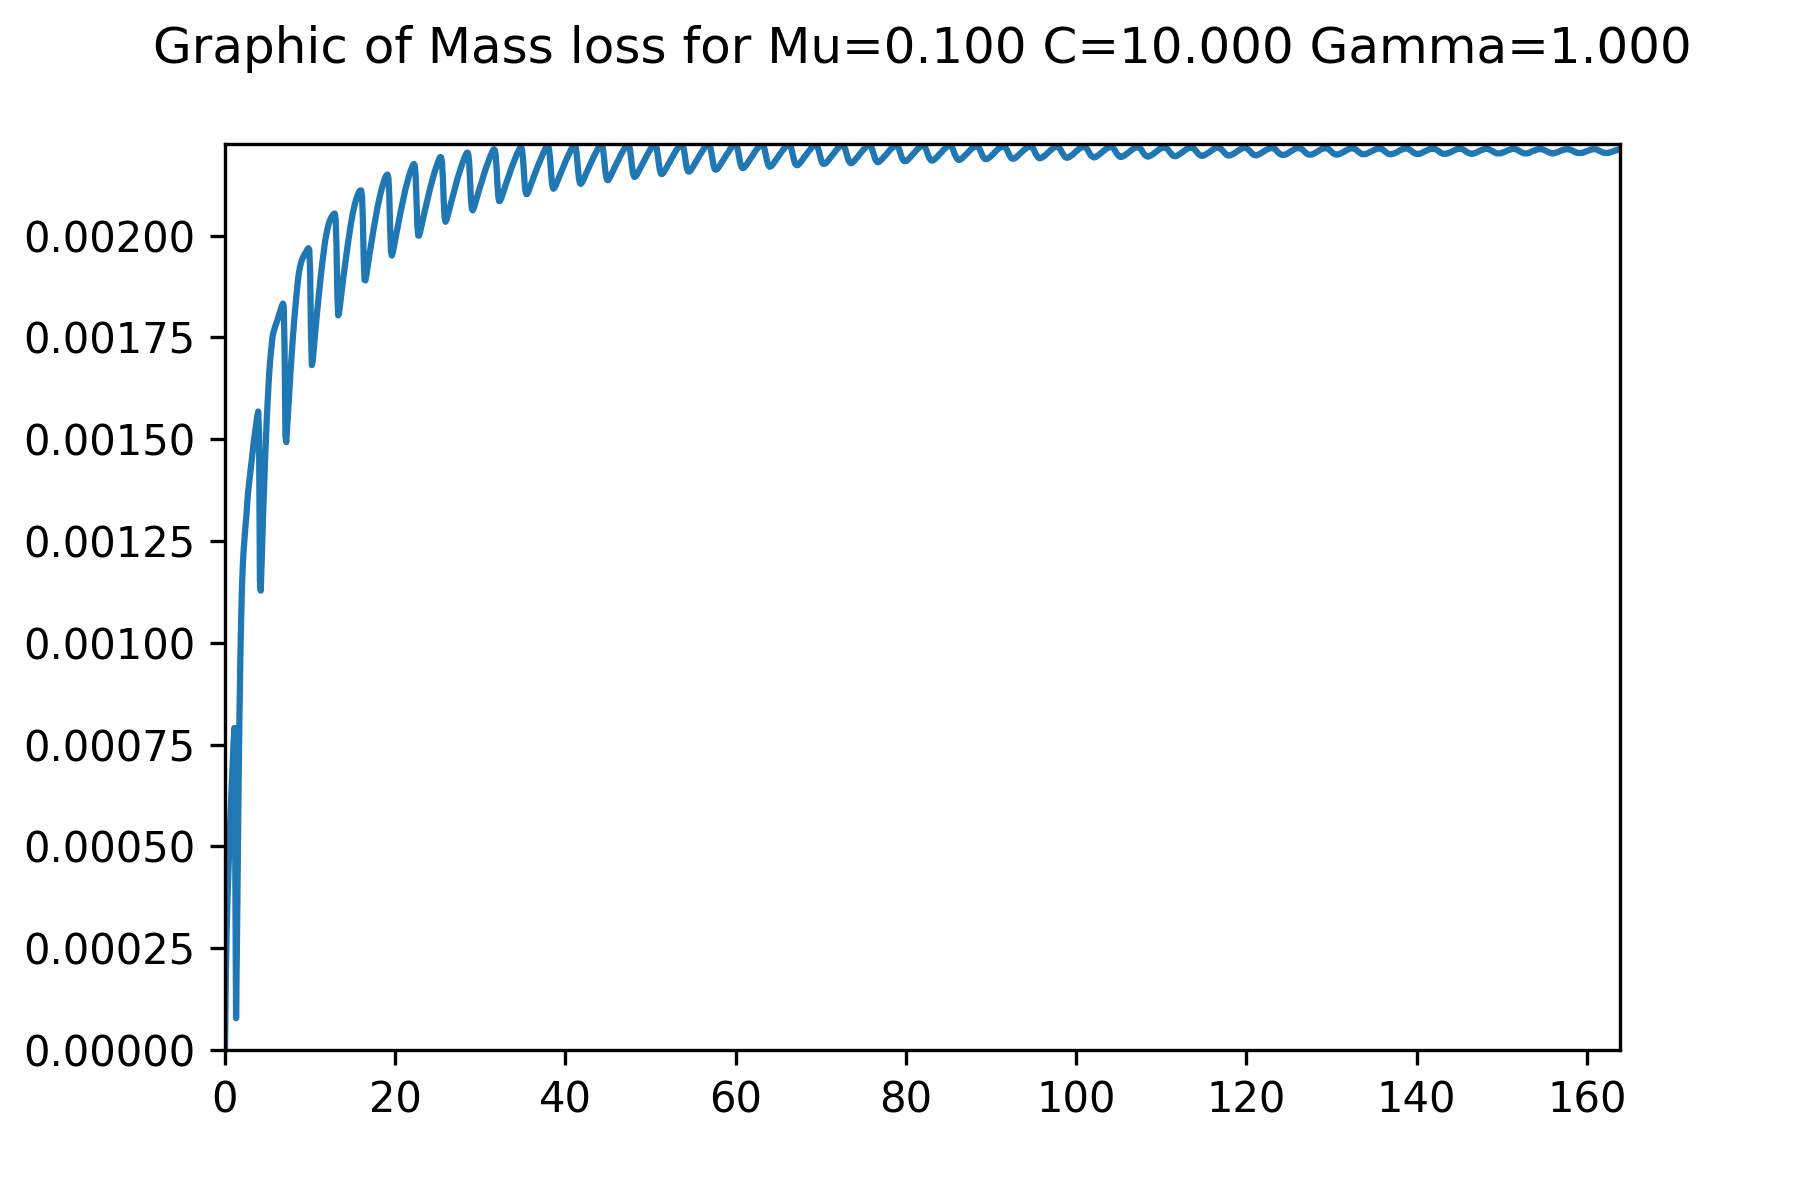
\includegraphics[scale=0.65]{../graphs_data_nonsmooth_1/mass/Graph_mass_mu0.100_C10.000_gamma1.000.png}
	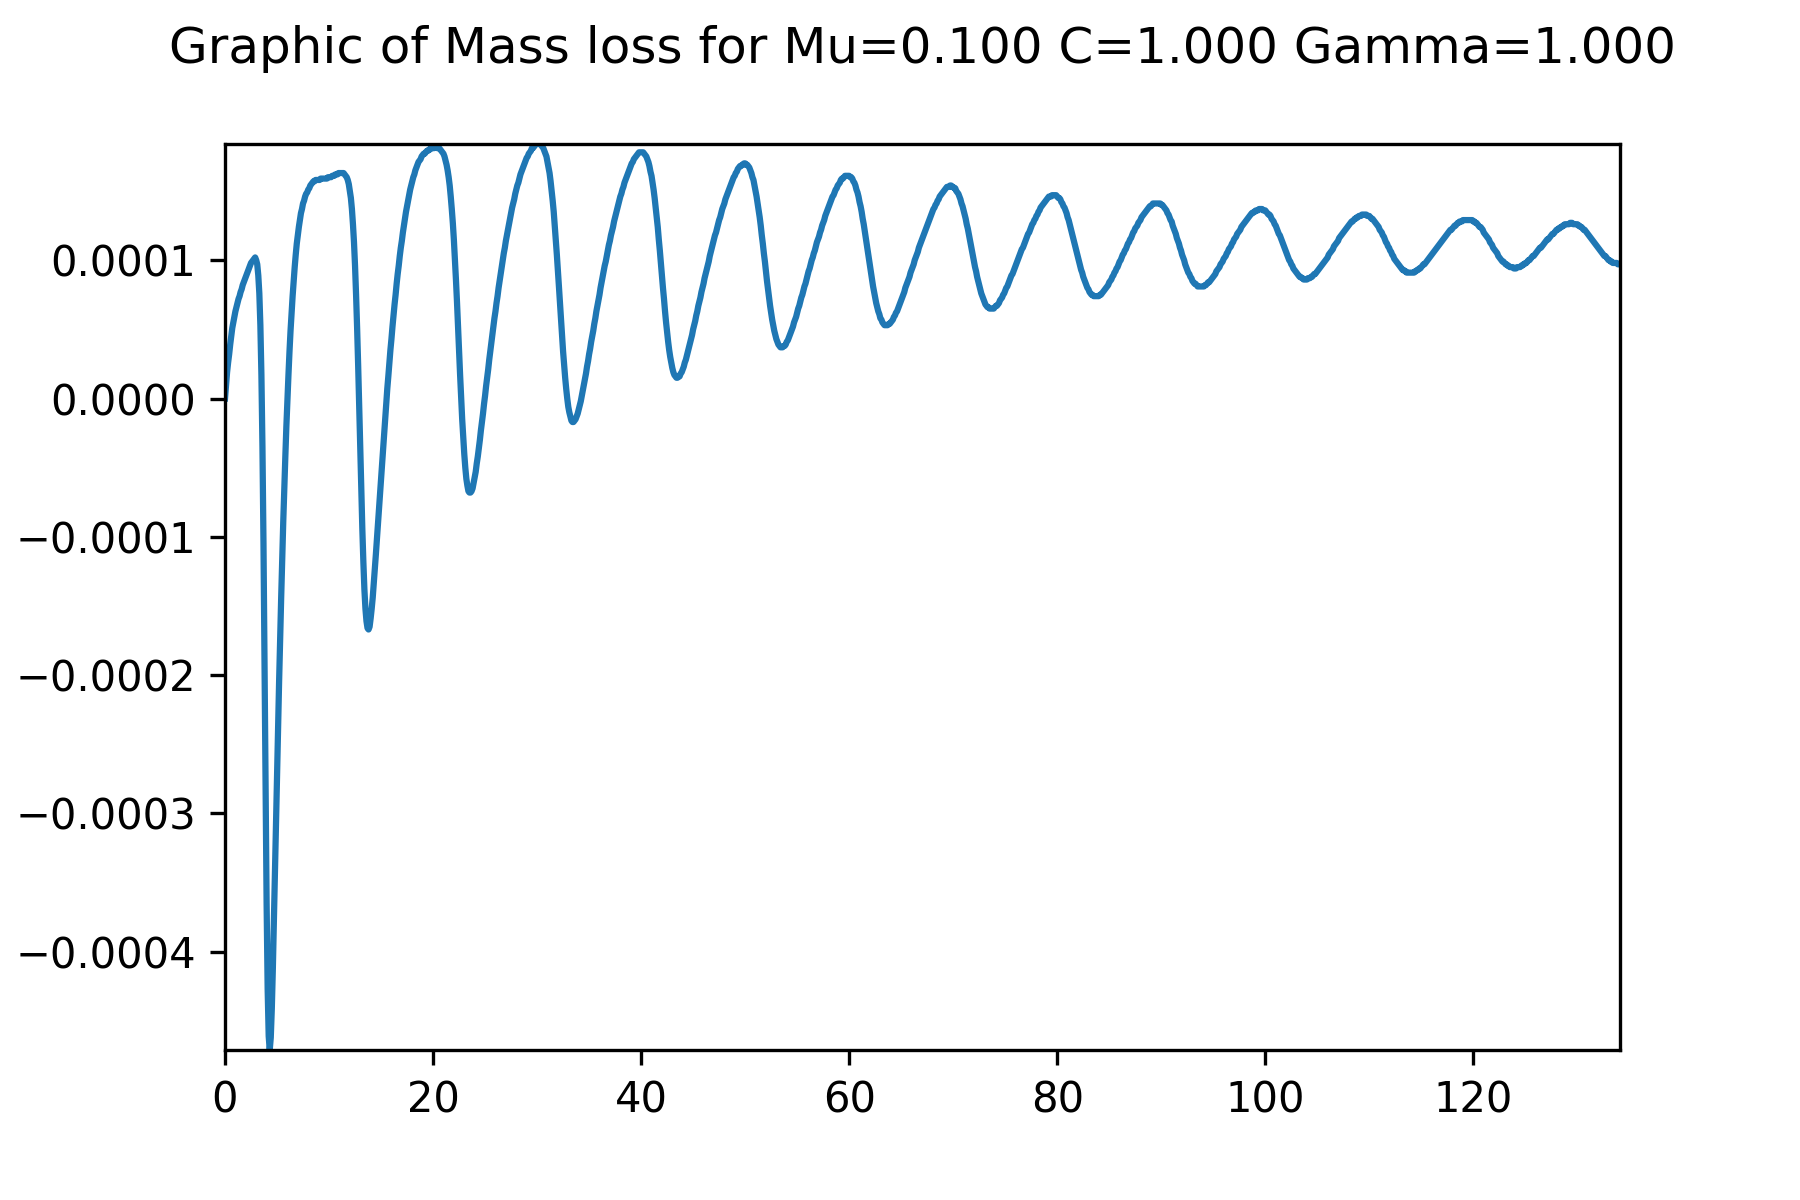
\includegraphics[scale=0.65]{../graphs_data_nonsmooth_1/mass/Graph_mass_mu0.100_C1.000_gamma1.000.png}	
	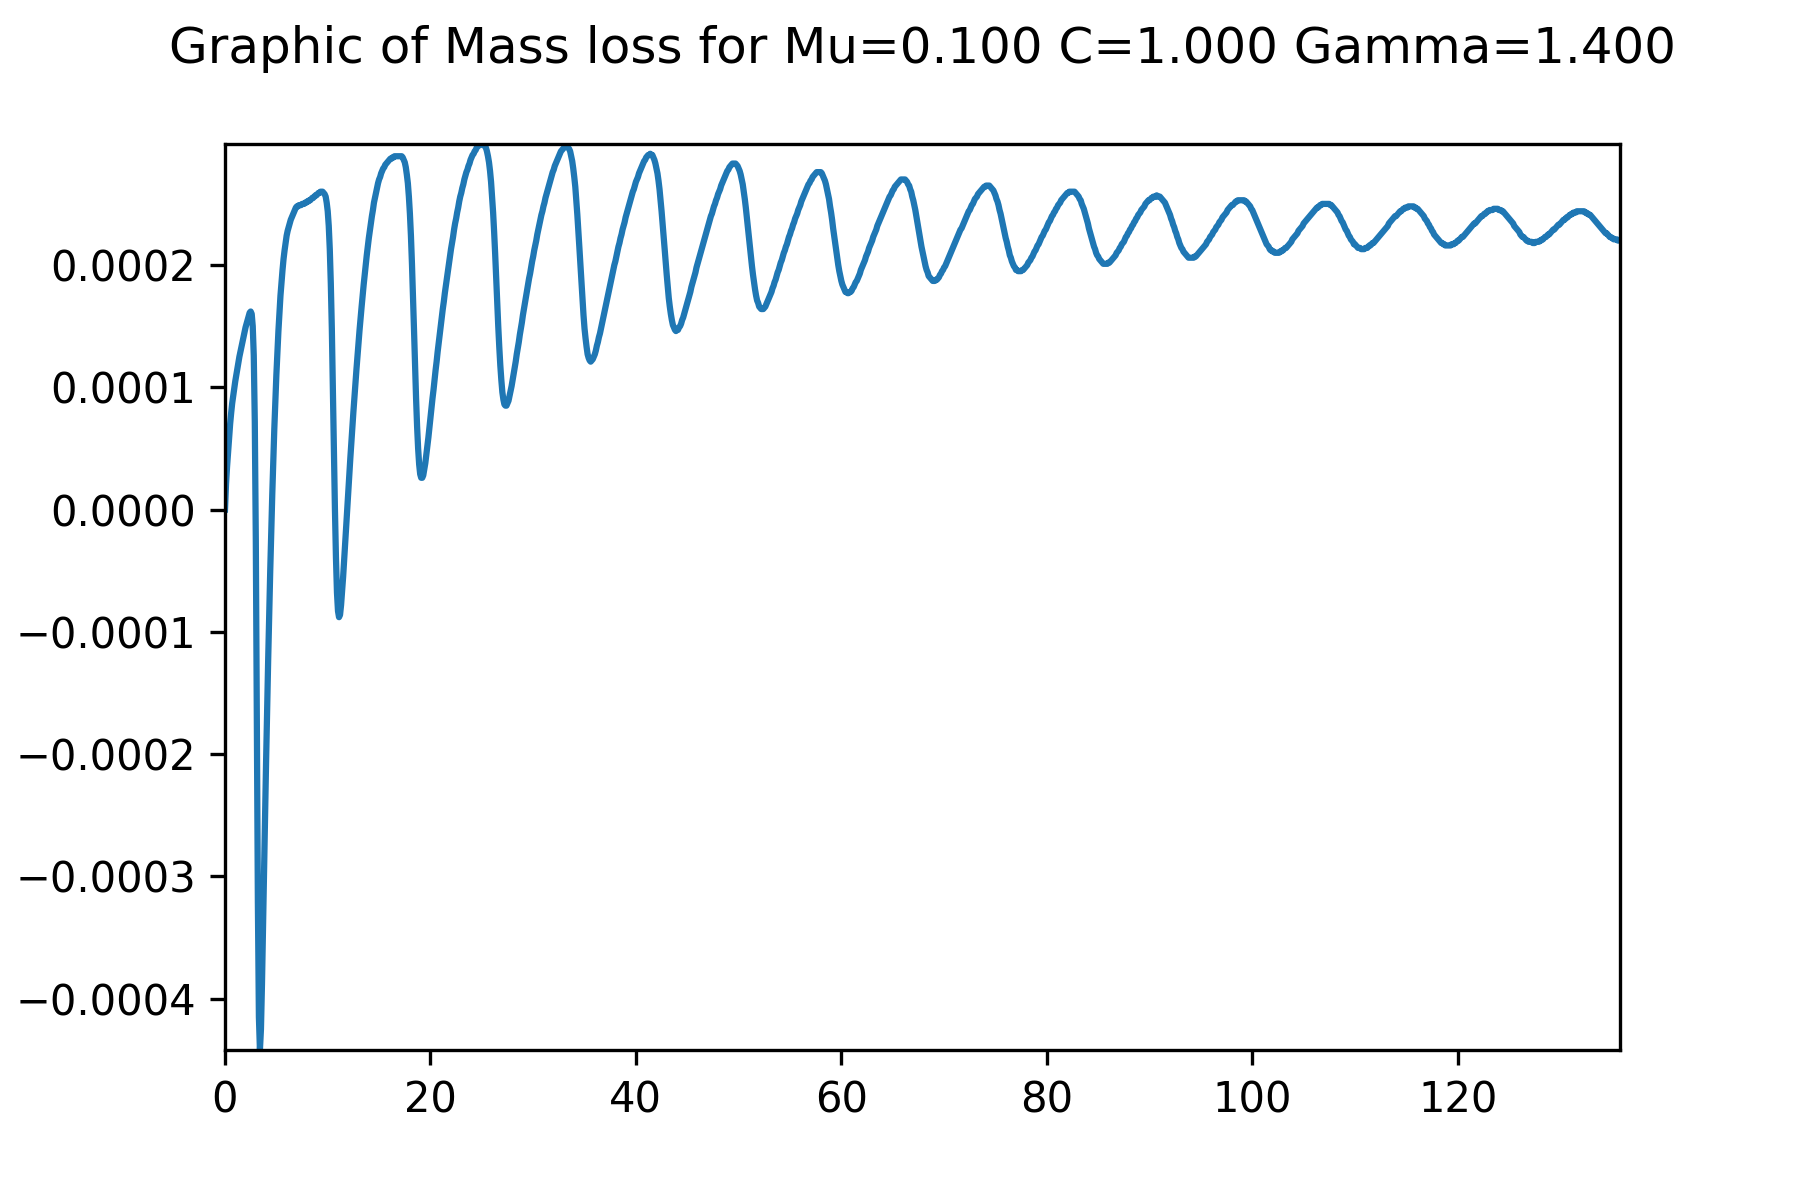
\includegraphics[scale=0.65]{../graphs_data_nonsmooth_1/mass/Graph_mass_mu0.100_C1.000_gamma1.400.png}
\end{figure}


\begin{figure}[H]
	\centering
	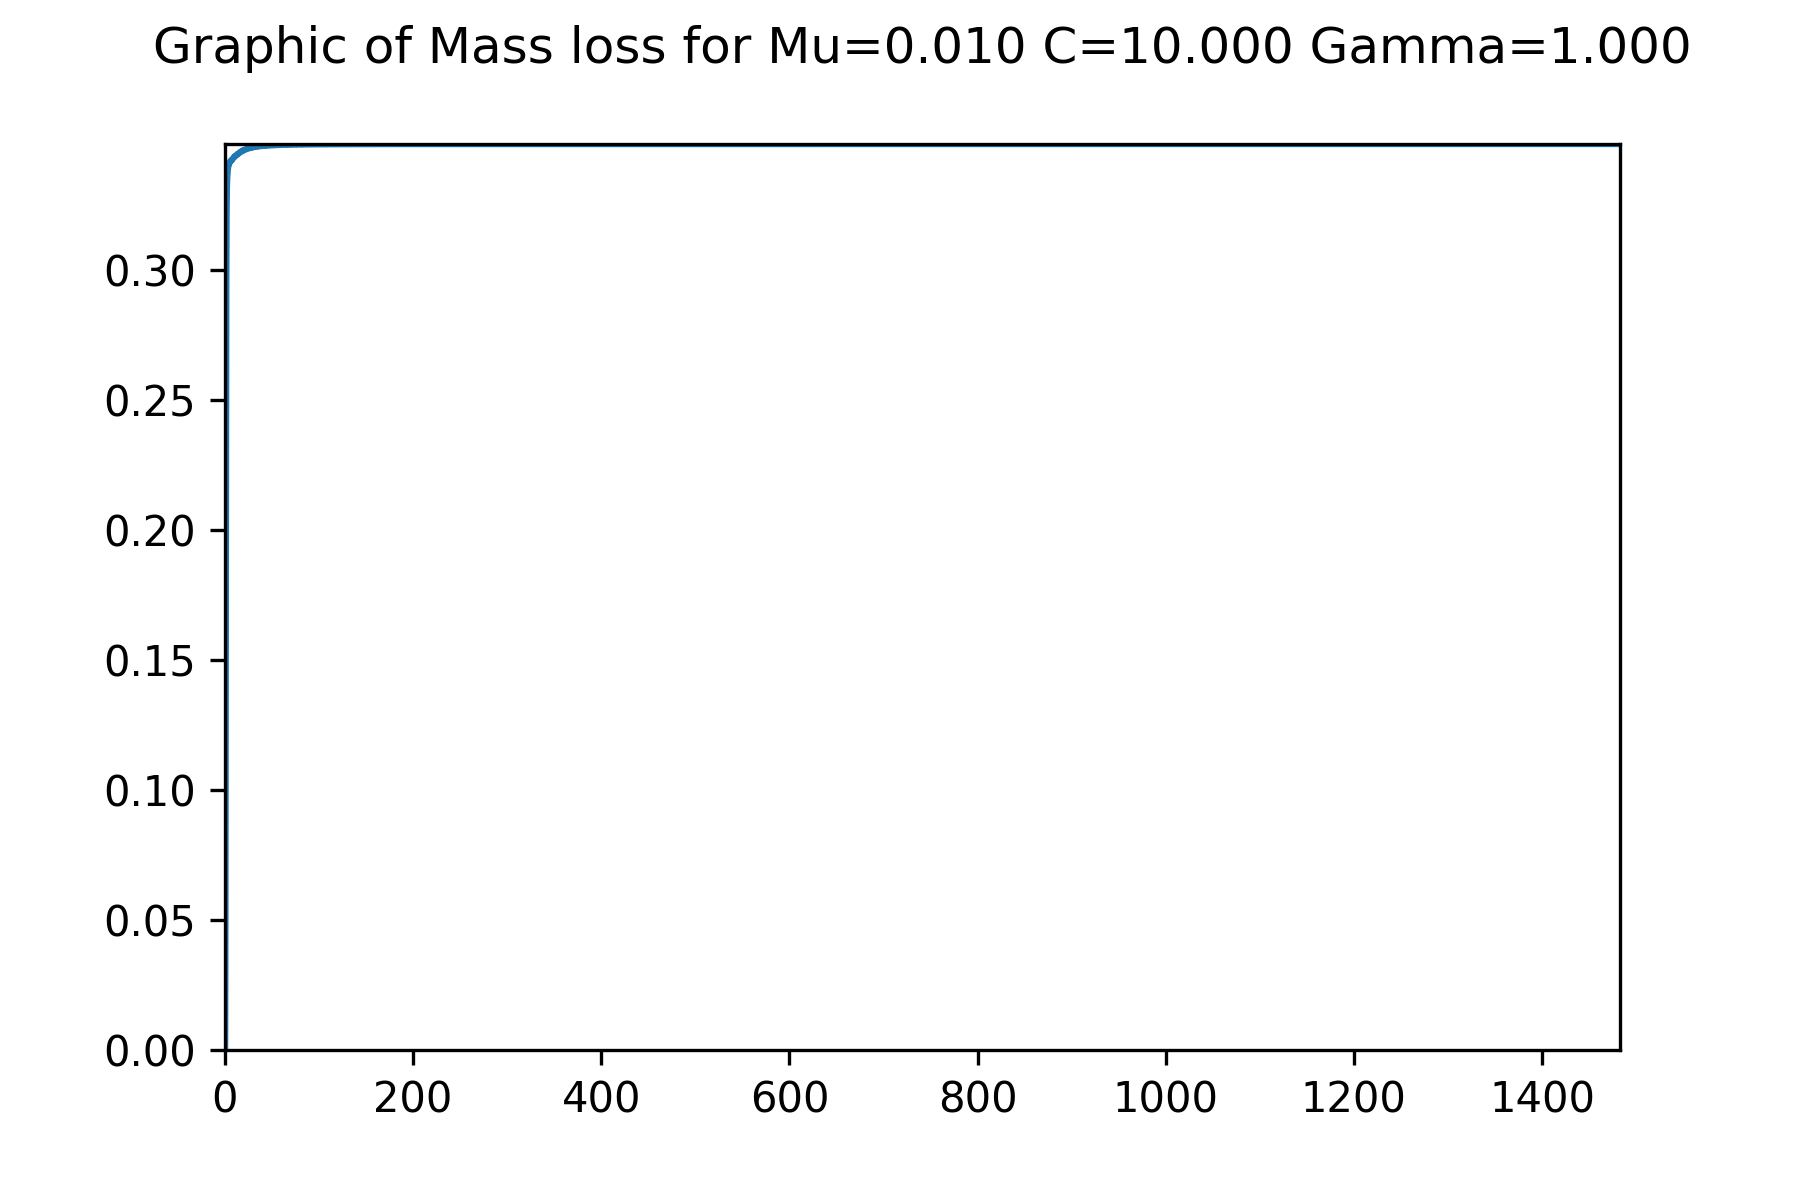
\includegraphics[scale=0.65]{../graphs_data_nonsmooth_1/mass/Graph_mass_mu0.010_C10.000_gamma1.000.png}
	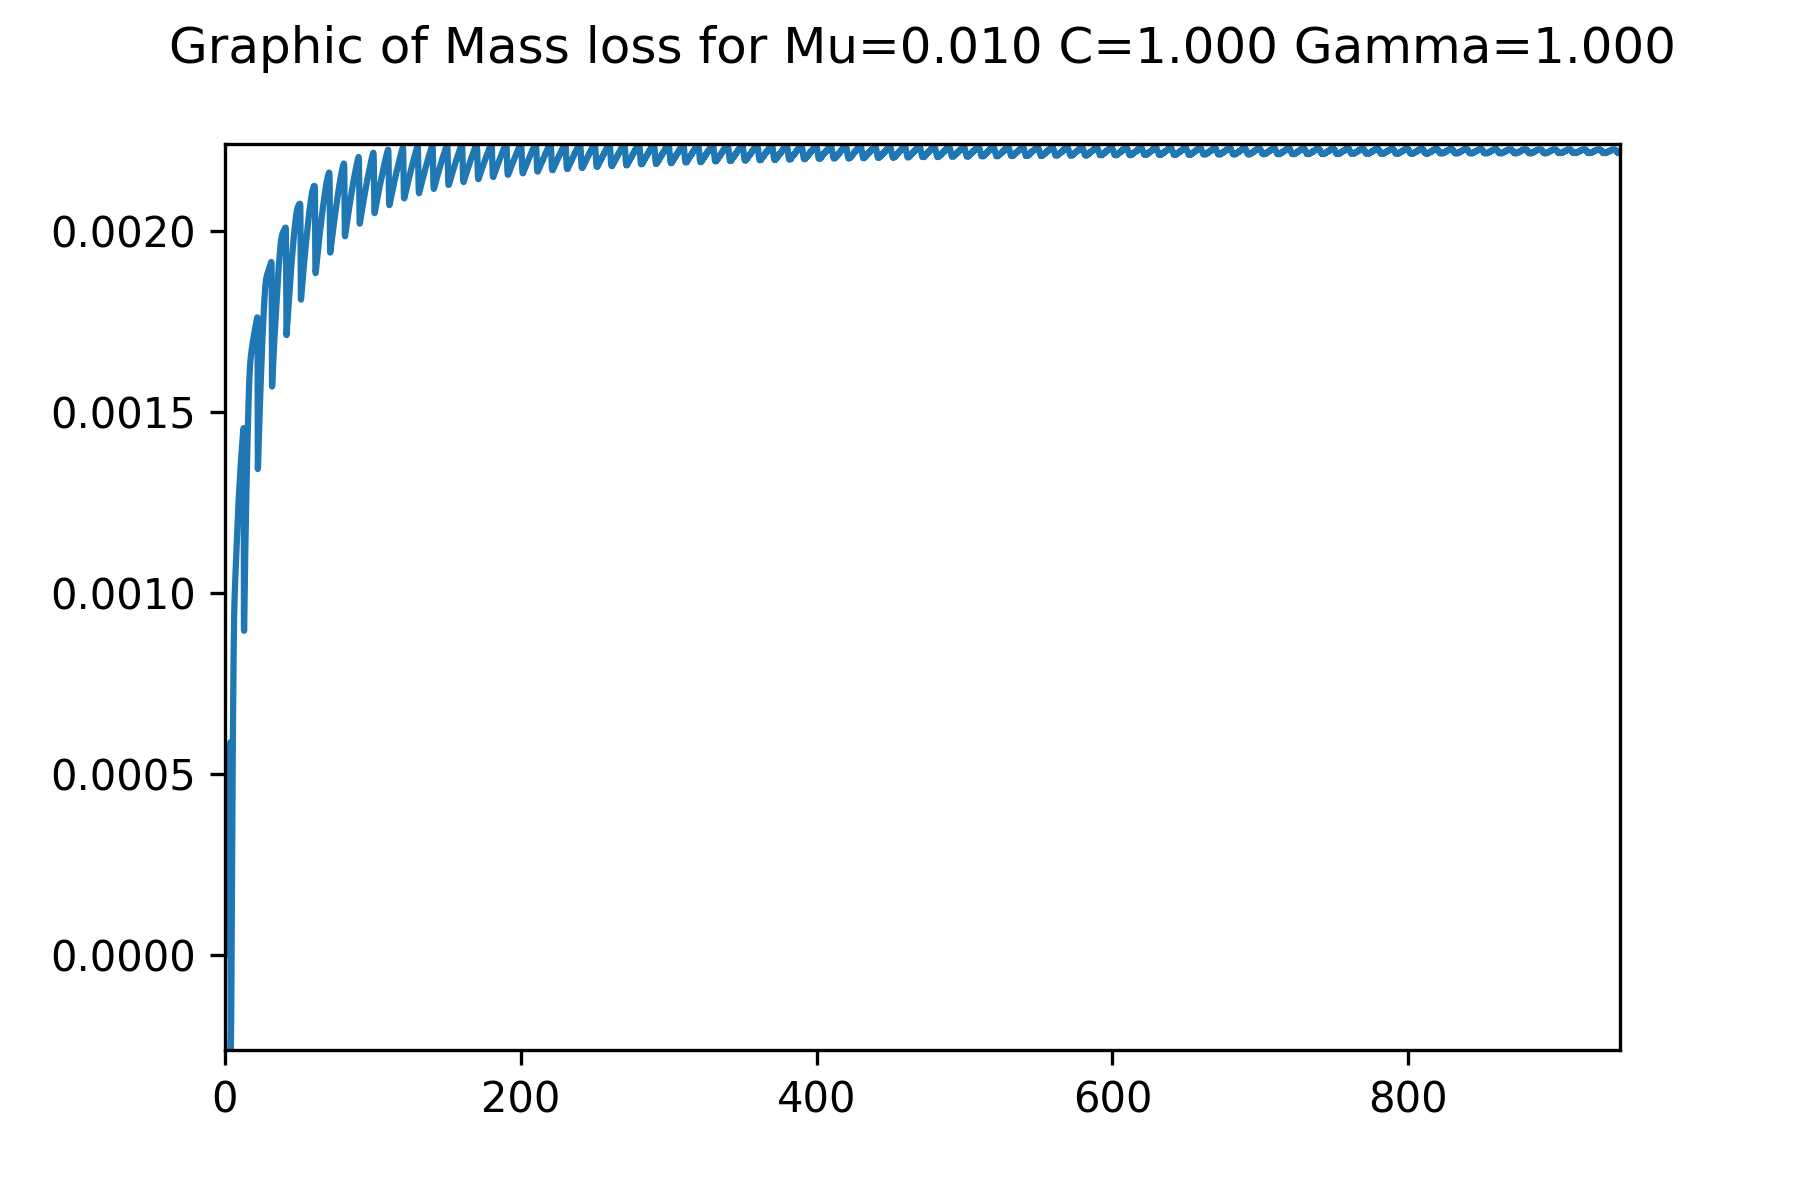
\includegraphics[scale=0.65]{../graphs_data_nonsmooth_1/mass/Graph_mass_mu0.010_C1.000_gamma1.000.png}	
	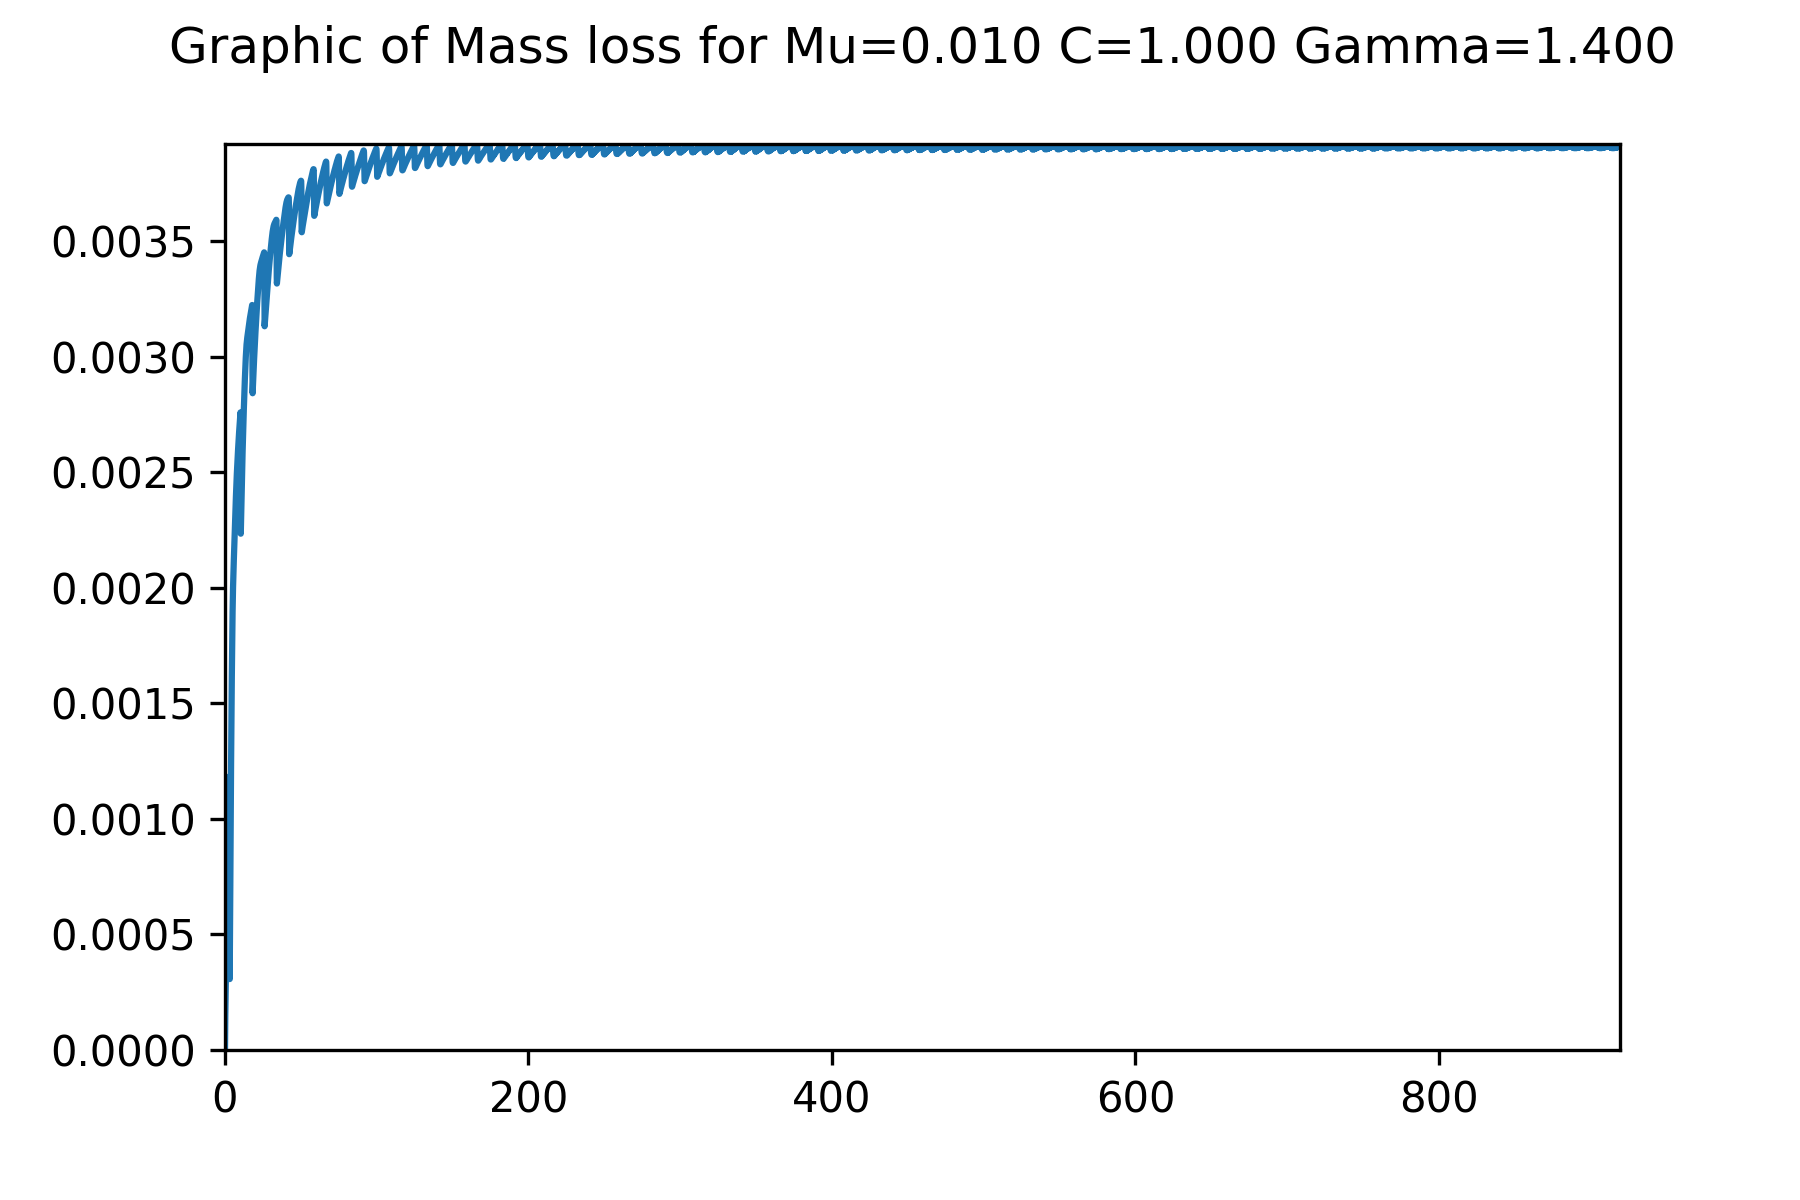
\includegraphics[scale=0.65]{../graphs_data_nonsmooth_1/mass/Graph_mass_mu0.010_C1.000_gamma1.400.png}
\end{figure}

Как можно заметить по таблицам потери массы составляют меньше 1-2\%, из чего можно заключить, что закон сохранения массы выполняется. \\

\newpage
\subsubsection{Вторая негладкая задача}
Ниже приведены таблицы времени стабилизации в зависимости от разных параметров $\mu$, $C$, $\gamma$

\begin{center}
Table of norms for H. $\mu = 0.0100$ \, $C = 10.0000$, $\gamma = 1.0000$
  
\begin{tabular}{|p{1in}|p{1in}|p{1in}|p{1in}|p{1in}|} \hline
$\tau / h$ &1.000e-01 &1.000e-02 &1.000e-03 &1.000e-04 \\ \hline 
1.000e-01 & $2.159e+01$  $9.587e+00$  $1.198e+02$  & $2.471e+02$  $3.984e+01$  $4.609e+03$  & $2.133e+05$  $8.964e+03$  $1.237e+07$  & $9.071e+06$  $9.628e+04$  $1.372e+09$  \\ \hline 
1.000e-02 & $3.757e+01$  $1.960e+01$  $2.769e+02$  & $7.268e+03$  $7.591e+02$  $1.296e+05$  & $4.183e+03$  $2.453e+02$  $3.613e+05$  & $1.706e+04$  $5.245e+02$  $7.946e+06$  \\ \hline 
1.000e-03 & $8.250e+01$  $5.484e+01$  $9.331e+02$  & $5.382e+01$  $2.538e+01$  $3.733e+03$  & $nan$  $-nan$  $-nan$  & $nan$  $-nan$  $-nan$  \\ \hline 
1.000e-04 & $6.557e+01$  $4.134e+01$  $6.523e+02$  & $4.257e-03$  $2.137e-03$  $3.011e-02$  & $nan$  $-nan$  $-nan$  & $nan$  $-nan$  $-nan$  \\ \hline 

\end{tabular}\\[20pt]
\end{center}

\begin{center}
Table of norms for H. $\mu = 0.0100$ \, $C = 1.0000$, $\gamma = 1.0000$
  
\begin{tabular}{|p{1in}|p{1in}|p{1in}|p{1in}|p{1in}|} \hline
$\tau / h$ &1.000e-01 &1.000e-02 &1.000e-03 &1.000e-04 \\ \hline 
1.000e-01 & $6.402e+00$  $3.503e+00$  $6.085e+01$  & $1.104e+02$  $1.829e+01$  $2.648e+03$  & $5.696e+07$  $2.433e+06$  $3.442e+09$  & $4.113e+07$  $1.169e+06$  $1.652e+10$  \\ \hline 
1.000e-02 & $1.294e+01$  $6.238e+00$  $1.109e+02$  & $3.998e+01$  $7.511e+00$  $1.111e+03$  & $1.491e+03$  $9.452e+01$  $1.439e+05$  & $nan$  $-nan$  $-nan$  \\ \hline 
1.000e-03 & $1.213e+01$  $7.867e+00$  $1.109e+02$  & $1.218e-02$  $4.318e-03$  $1.627e-01$  & $nan$  $nan$  $nan$  & $nan$  $nan$  $nan$  \\ \hline 
1.000e-04 & $1.310e+01$  $8.536e+00$  $1.386e+02$  & $5.115e-03$  $2.362e-03$  $4.356e-02$  & $nan$  $-nan$  $-nan$  & $nan$  $nan$  $nan$  \\ \hline 

\end{tabular}\\[20pt]
\end{center}

\begin{center}
Table of norms for V. $\mu = 0.0100$ \, $C = 1.0000$, $\gamma = 1.4000$
  
\begin{tabular}{|p{0.8in}|p{0.8in}|p{0.8in}|p{0.8in}|p{0.8in}|p{0.8in}|p{0.8in}|} \hline
$K$ &$N_0$ &$N_0 \tau$ &$n = \frac{N_0}{4}$ &$n = \frac{N_0}{2}$ &$n = \frac{3N_0}{4}$ &$n = N_0$ \\ \hline 
0 &919330 &9.193e+02 &1.980e-02 &8.076e-03 &6.651e-03 &9.998e-04 \\ \hline 
1 &1838659 &9.193e+02 &1.891e-02 &8.395e-03 &5.863e-03 &1.467e-03 \\ \hline 
2 &3677317 &9.193e+02 &1.853e-02 &8.487e-03 &5.518e-03 &1.632e-03 \\ \hline 
3 &7354633 &9.193e+02 &1.835e-02 &8.521e-03 &5.358e-03 &1.701e-03 \\ \hline 

\end{tabular}\\[20pt]
\end{center}


\newpage
\begin{center}
Table of norms for V. $\mu = 0.1000$ \, $C = 10.0000$, $\gamma = 1.0000$
  
\begin{tabular}{|p{0.8in}|p{0.8in}|p{0.8in}|p{0.8in}|p{0.8in}|p{0.8in}|p{0.8in}|} \hline
$K$ &$N_0$ &$N_0 \tau$ &$n = \frac{N_0}{4}$ &$n = \frac{N_0}{2}$ &$n = \frac{3N_0}{4}$ &$n = N_0$ \\ \hline 
0 &163946 &1.639e+02 &1.087e-01 &3.157e-02 &8.669e-03 &9.950e-04 \\ \hline 
1 &327891 &1.639e+02 &1.041e-01 &2.907e-02 &7.359e-03 &9.549e-04 \\ \hline 
2 &655781 &1.639e+02 &1.018e-01 &2.785e-02 &6.758e-03 &9.451e-04 \\ \hline 
3 &1311561 &1.639e+02 &1.007e-01 &2.724e-02 &6.465e-03 &9.426e-04 \\ \hline 

\end{tabular}\\[20pt]
\end{center}

\begin{center}
Table of norms for V. $\mu = 0.1000$ \, $C = 1.0000$, $\gamma = 1.0000$
  
\begin{tabular}{|p{1in}|p{1in}|p{1in}|p{1in}|p{1in}|} \hline
$\tau / h$ &1.000e-01 &1.000e-02 &1.000e-03 &1.000e-04 \\ \hline 
1.000e-01 & $5.855e+00$  $3.789e+00$  $6.347e+01$  & $2.239e+00$  $1.058e+00$  $3.760e+01$  & $1.067e+01$  $5.882e+00$  $2.601e+01$  & $1.850e+00$  $9.454e-01$  $1.013e+01$  \\ \hline 
1.000e-02 & $9.409e+00$  $5.648e+00$  $8.658e+01$  & $2.318e-01$  $7.808e-02$  $1.927e+00$  & $2.597e-01$  $8.324e-02$  $2.107e+00$  & $2.676e-01$  $8.564e-02$  $2.166e+00$  \\ \hline 
1.000e-03 & $2.178e+01$  $1.149e+01$  $1.968e+02$  & $1.818e-02$  $6.728e-03$  $1.157e-01$  & $1.392e-02$  $5.080e-03$  $9.453e-02$  & $1.388e-02$  $5.066e-03$  $9.436e-02$  \\ \hline 
1.000e-04 & $4.808e+01$  $3.105e+01$  $4.787e+02$  & $5.519e-03$  $2.421e-03$  $3.727e-02$  & $1.376e-03$  $5.080e-04$  $9.219e-03$  & $1.337e-03$  $4.946e-04$  $9.061e-03$  \\ \hline 

\end{tabular}\\[20pt]
\end{center}

\begin{center}
Table of norms for V. $\mu = 0.1000$ \, $C = 1.0000$, $\gamma = 1.4000$
  
\begin{tabular}{|p{1in}|p{1in}|p{1in}|p{1in}|p{1in}|} \hline
$\tau / h$ &1.000e-01 &1.000e-02 &1.000e-03 &1.000e-04 \\ \hline 
1.000e-01 & $nan$  $nan$  $nan$  & $nan$  $-nan$  $-nan$  & $nan$  $-nan$  $-nan$  & $nan$  $-nan$  $-nan$  \\ \hline 
1.000e-02 & $nan$  $-nan$  $-nan$  & $1.079e-01$  $4.405e-02$  $1.733e+00$  & $8.880e-02$  $2.896e-02$  $1.526e+00$  & $8.242e-02$  $2.863e-02$  $1.415e+00$  \\ \hline 
1.000e-03 & $nan$  $nan$  $nan$  & $6.253e-03$  $3.009e-03$  $3.736e-02$  & $3.227e-03$  $1.517e-03$  $2.056e-02$  & $3.228e-03$  $1.507e-03$  $2.050e-02$  \\ \hline 
1.000e-04 & $nan$  $nan$  $nan$  & $3.758e-03$  $1.963e-03$  $2.731e-02$  & $3.241e-04$  $1.593e-04$  $2.093e-03$  & $3.202e-04$  $1.480e-04$  $2.016e-03$  \\ \hline 

\end{tabular}\\[20pt]
\end{center}


\newpage
Теперь рассмотрим динамику процесса на графиках затухания и временных срезах для различных значений параметров. 

\begin{figure}[H]
	\centering
	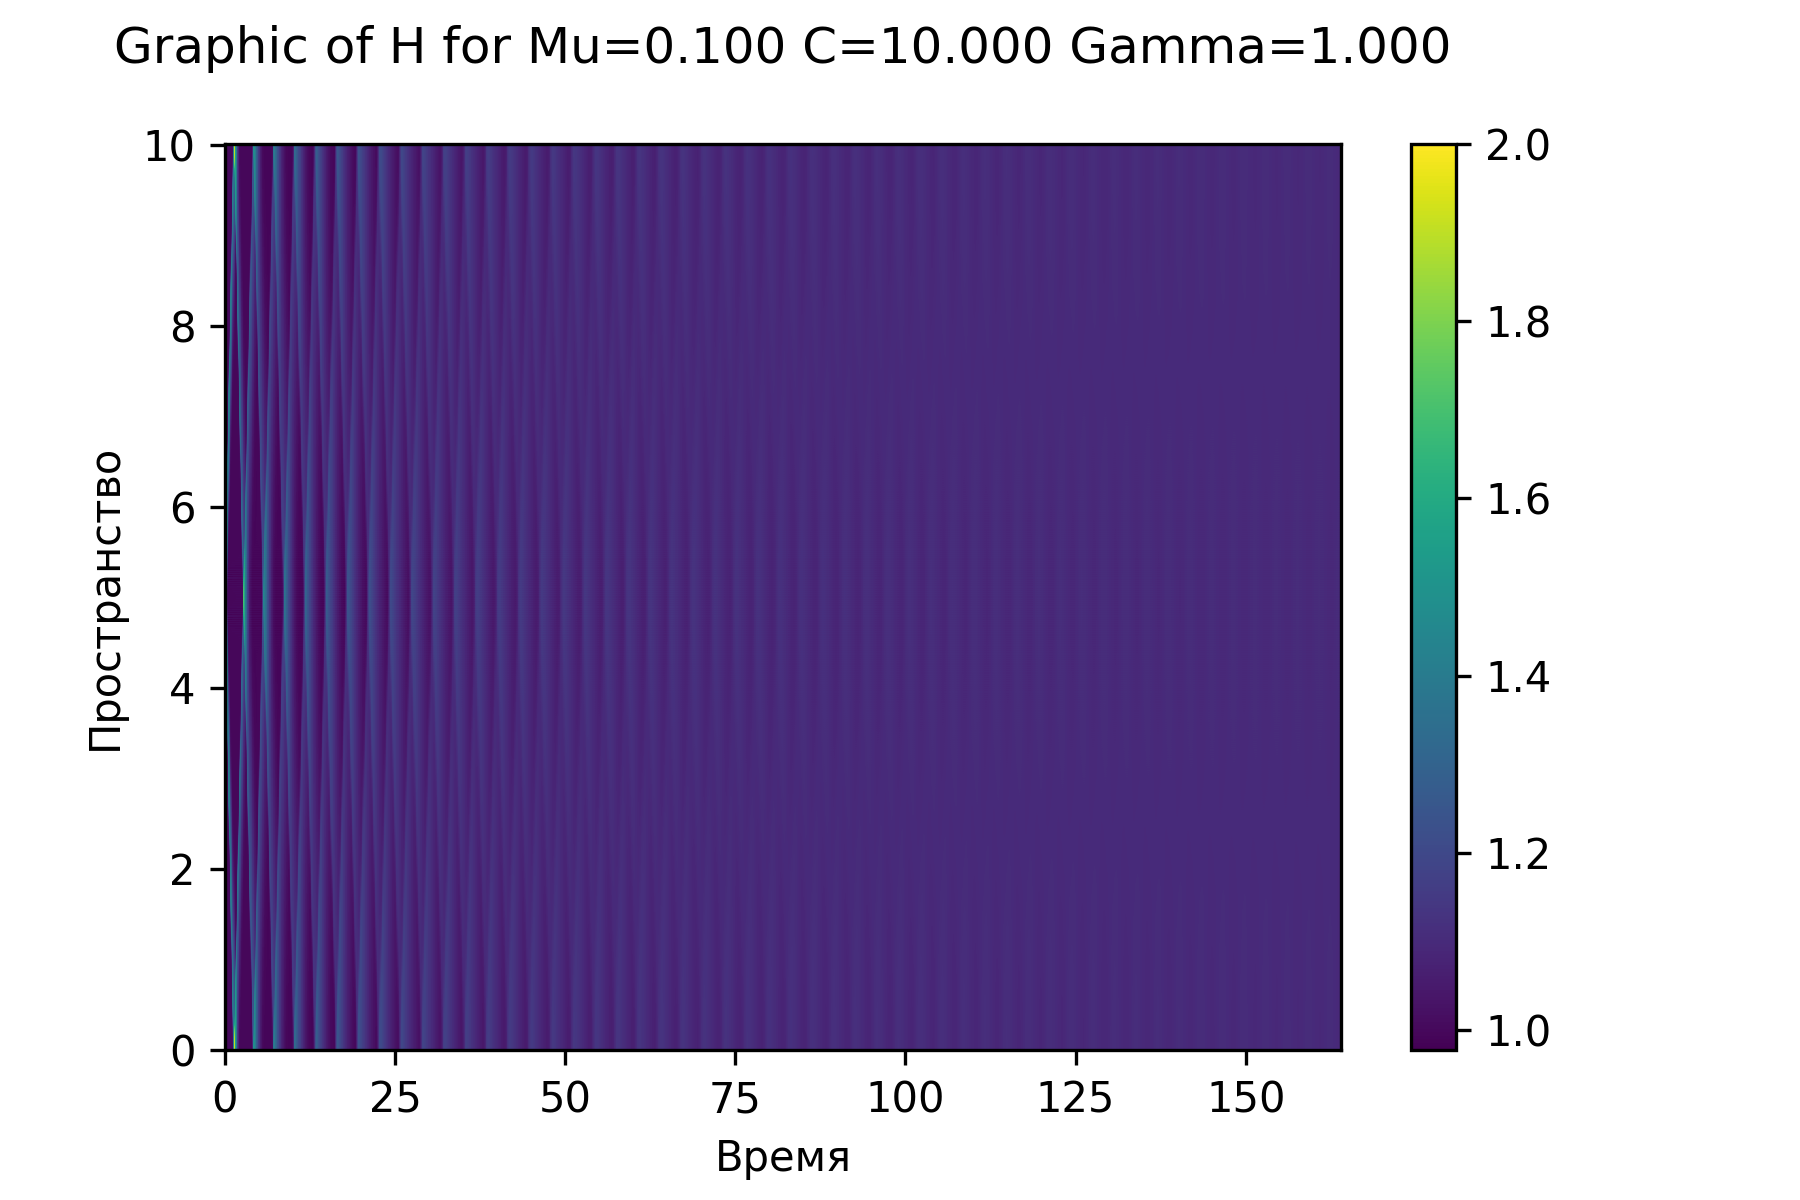
\includegraphics[scale=0.5]{../graphs_data_nonsmooth_2/value/Graph_H_mu0.010_C10.000_gamma1.000.png}
	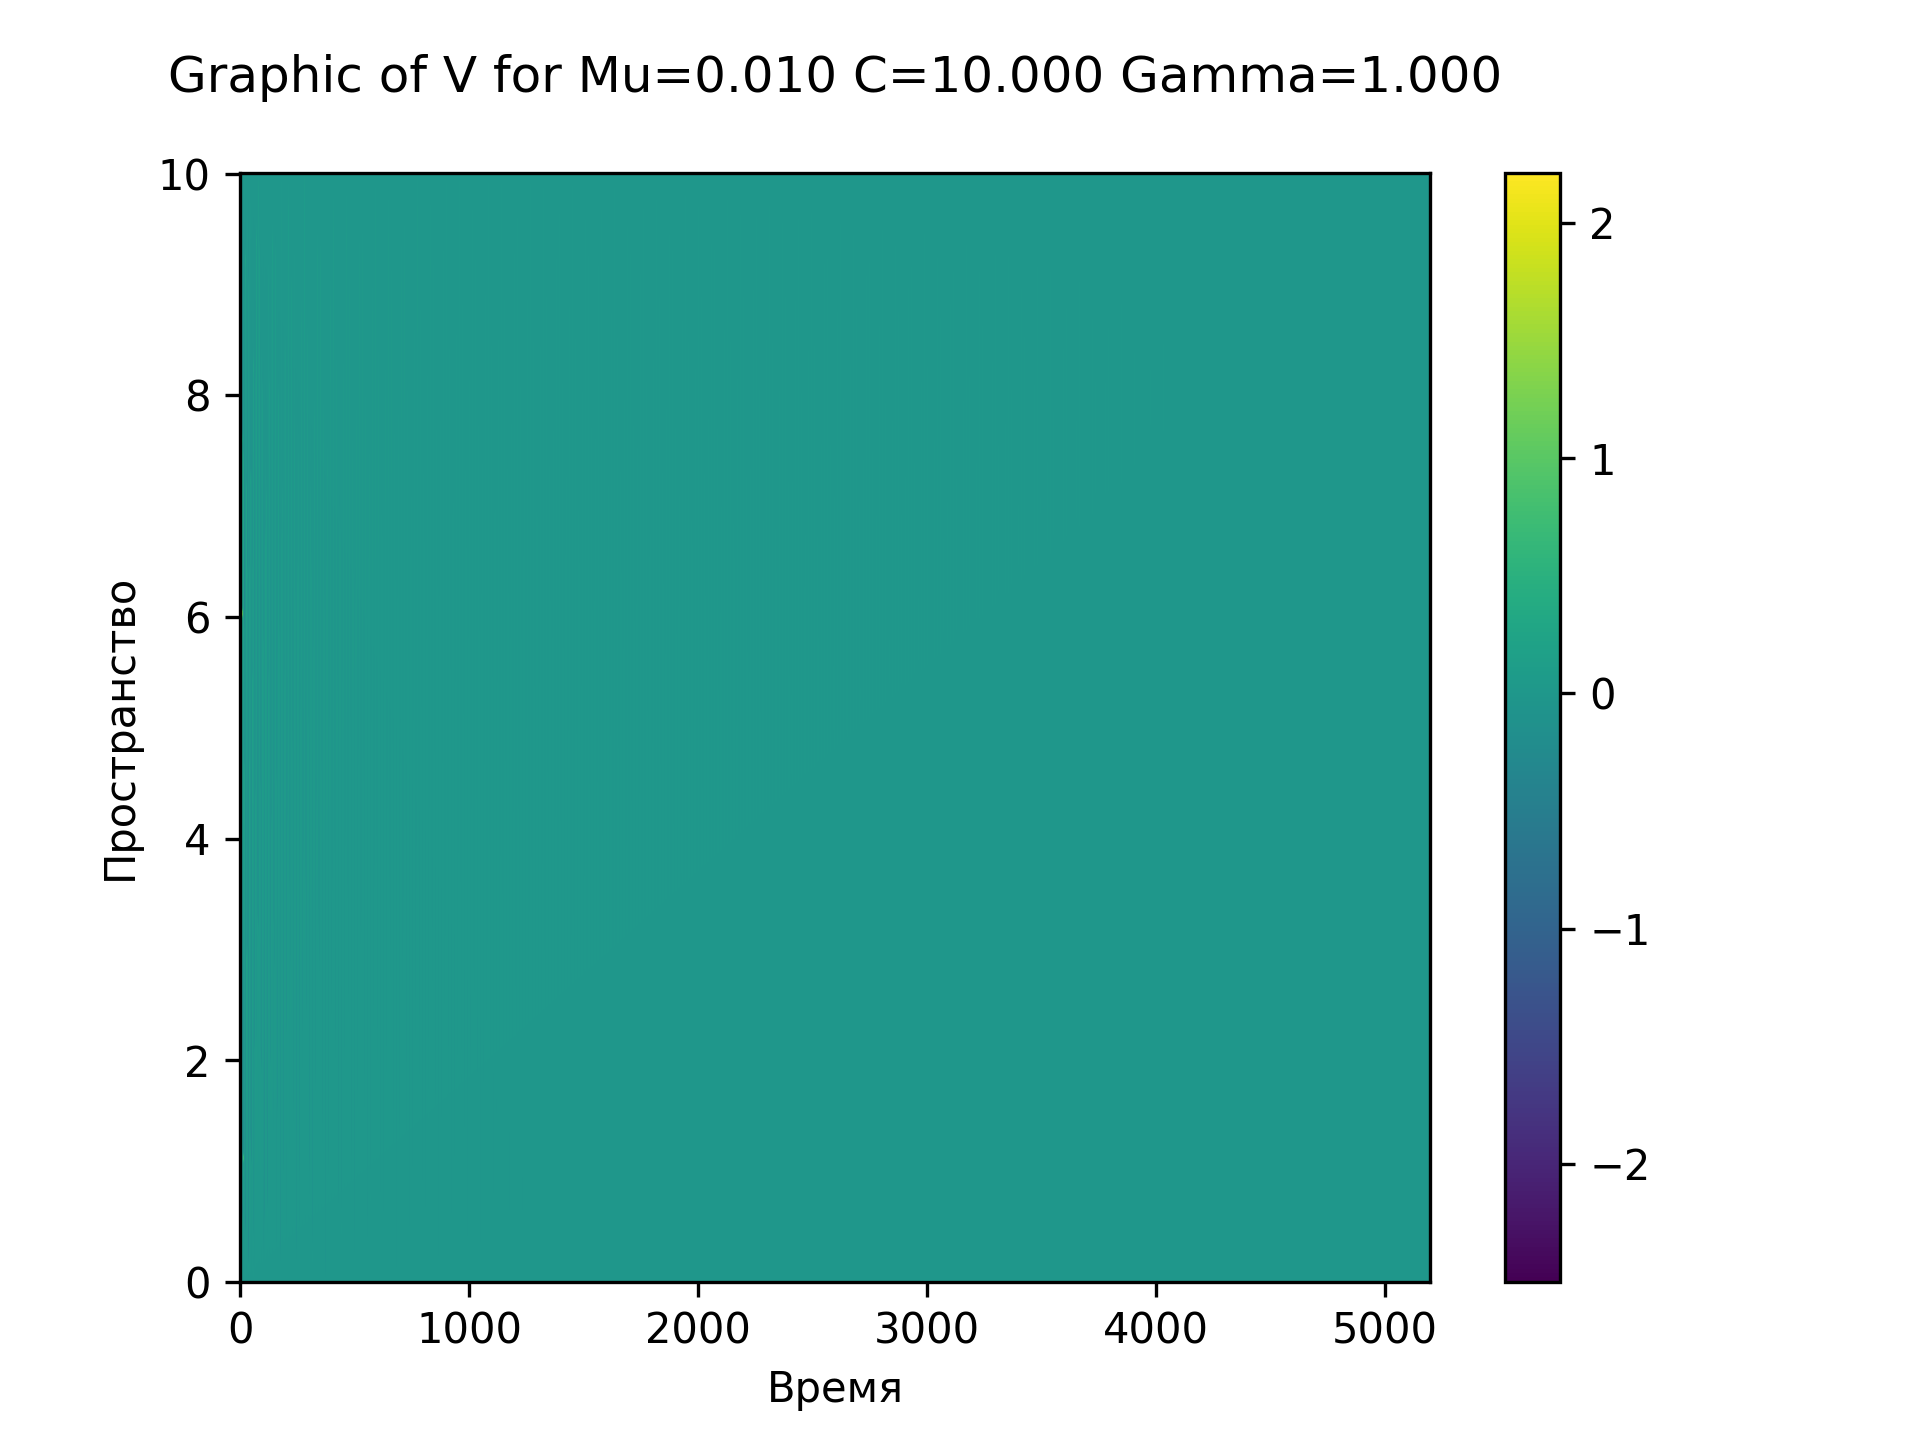
\includegraphics[scale=0.5]{../graphs_data_nonsmooth_2/value/Graph_V_mu0.010_C10.000_gamma1.000.png}	
	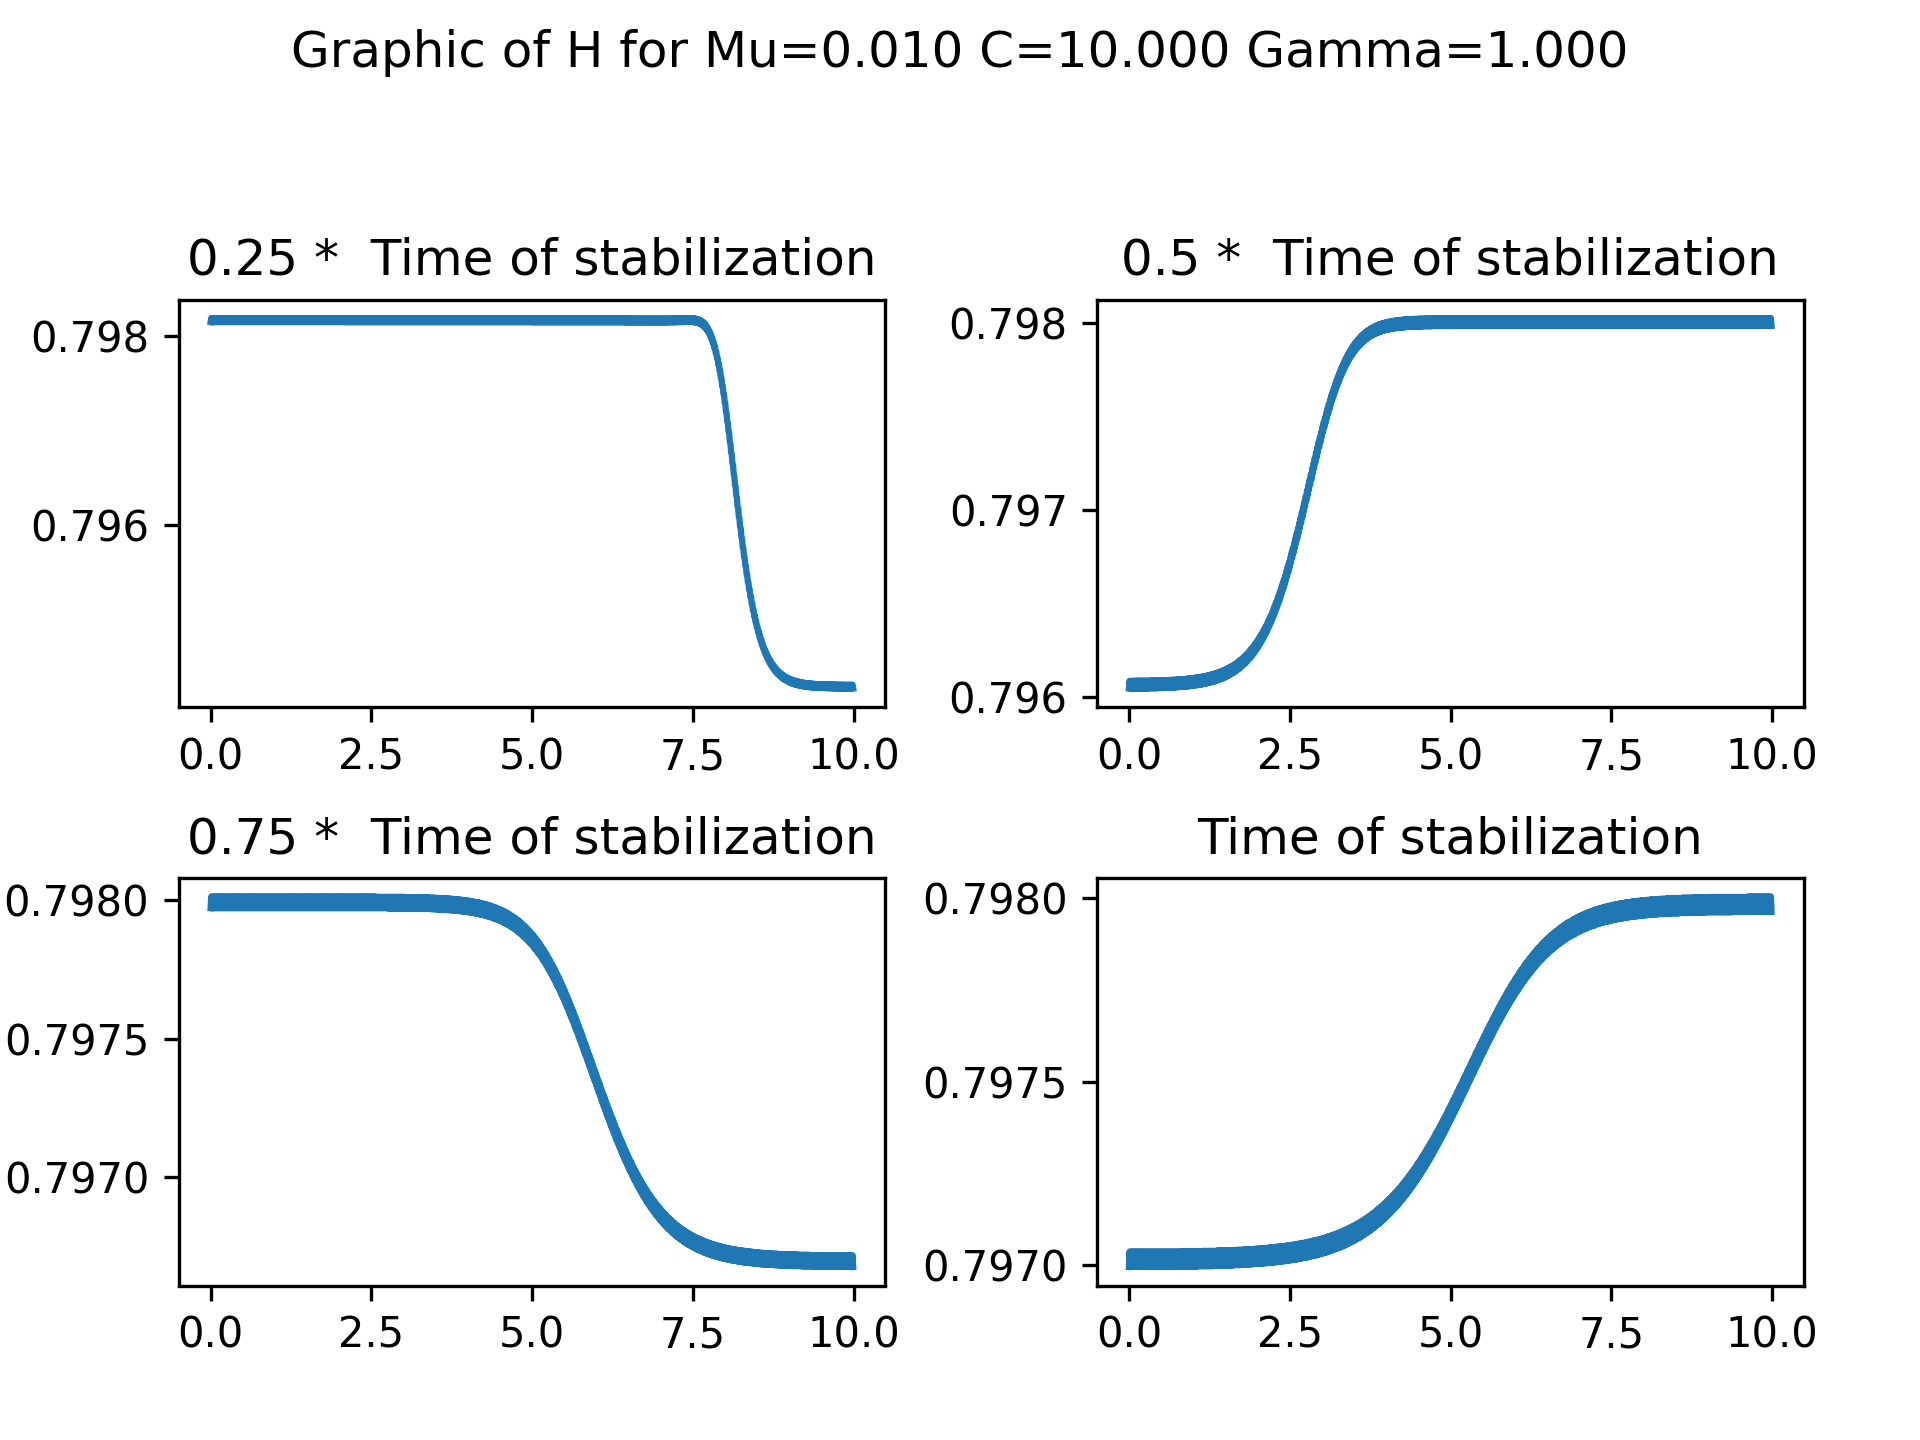
\includegraphics[scale=0.5]{../graphs_data_nonsmooth_2/slices/Graph_H_mu0.010_C10.000_gamma1.000.png}
	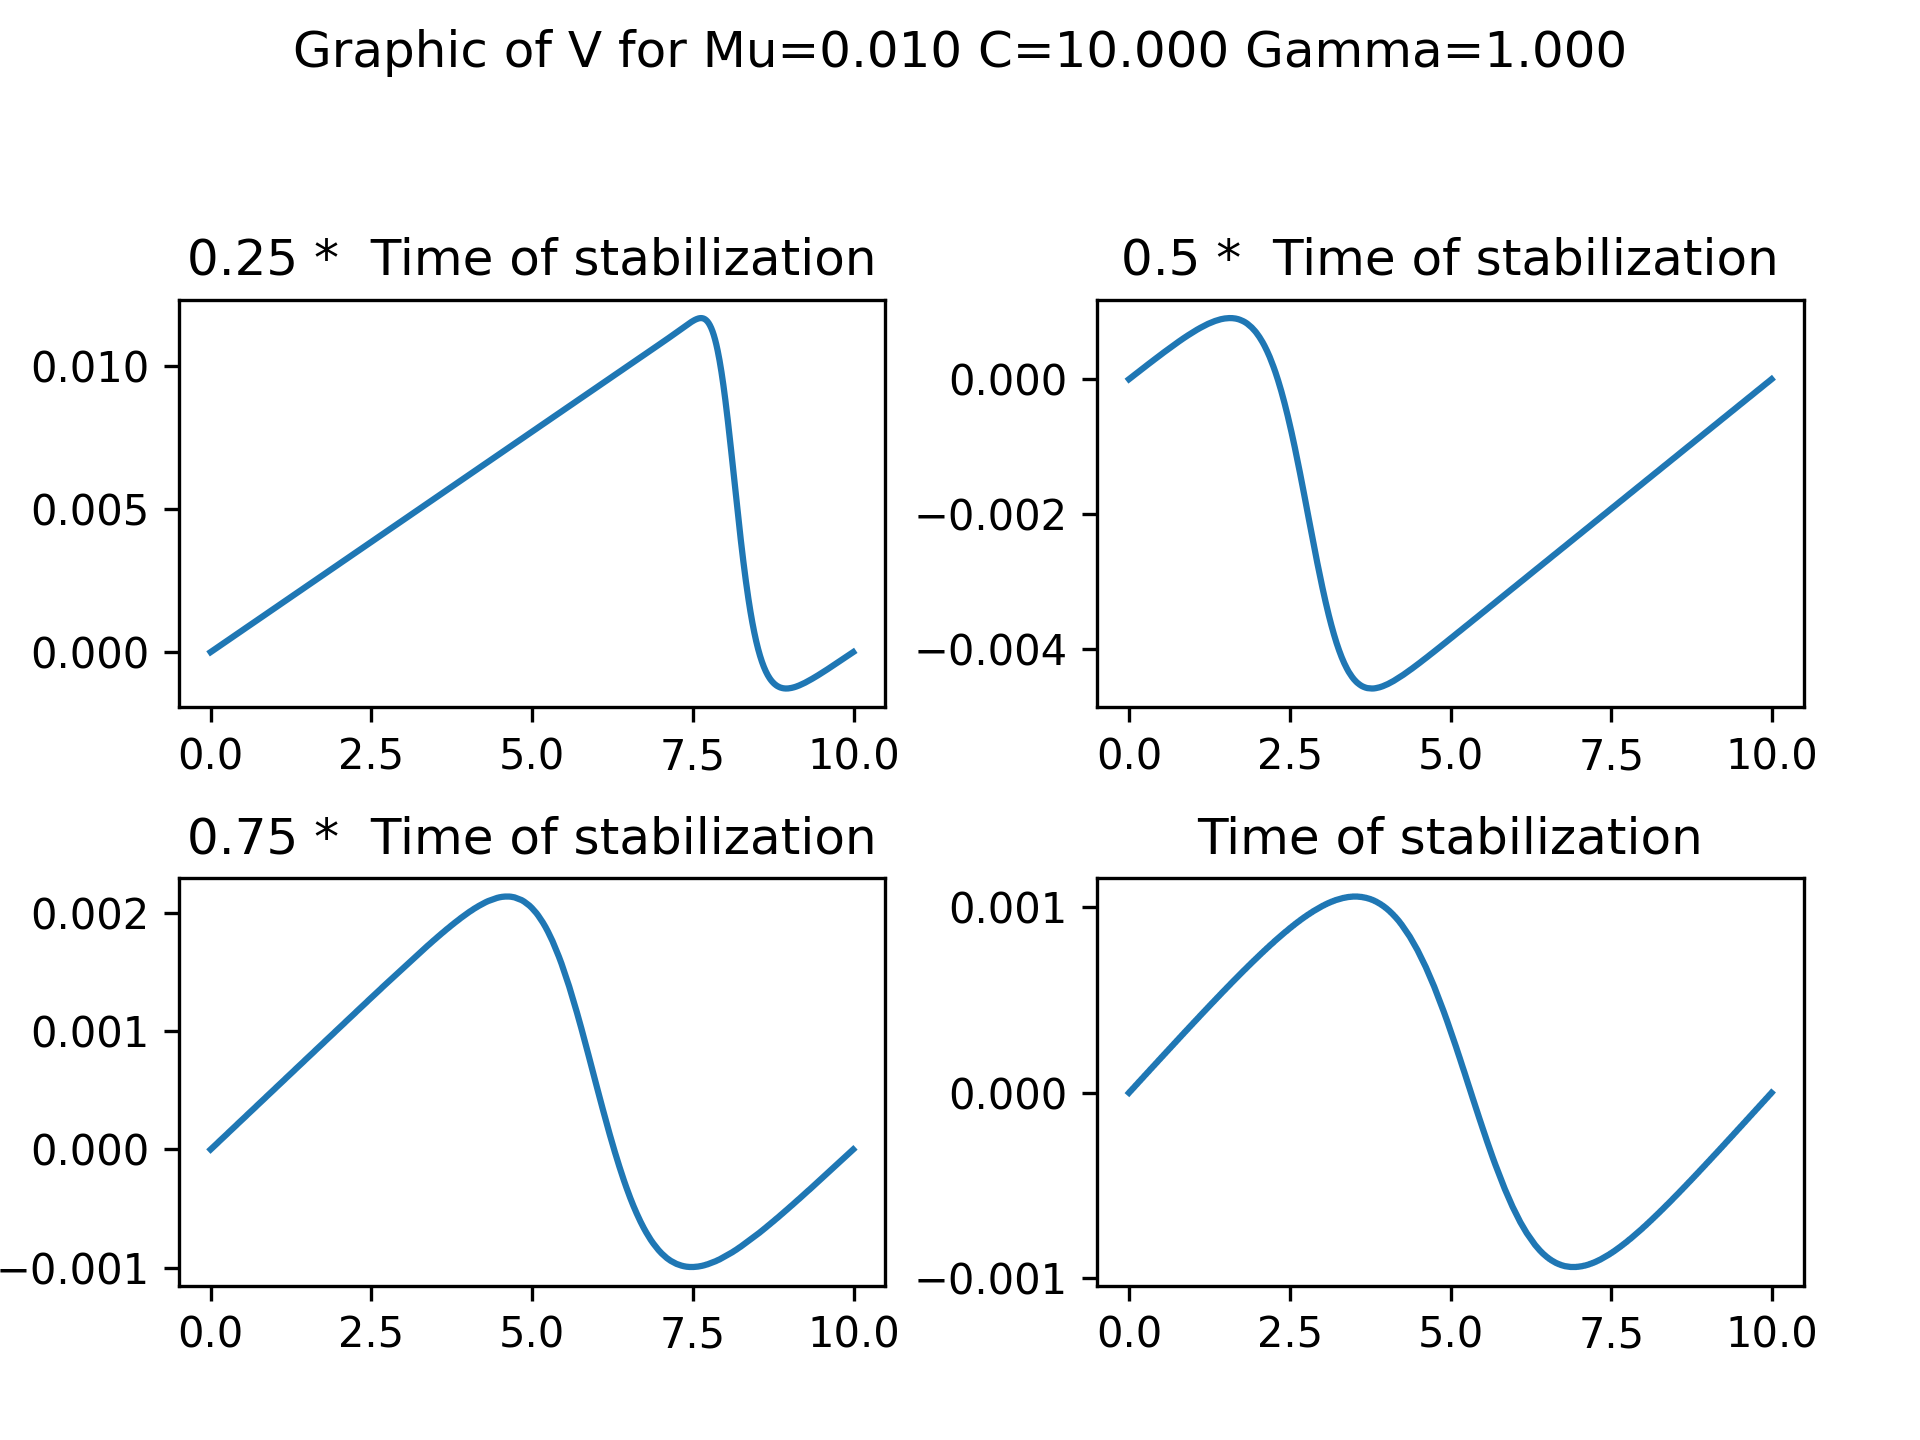
\includegraphics[scale=0.5]{../graphs_data_nonsmooth_2/slices/Graph_V_mu0.010_C10.000_gamma1.000.png}
\end{figure}

\begin{figure}[H]
	\centering
	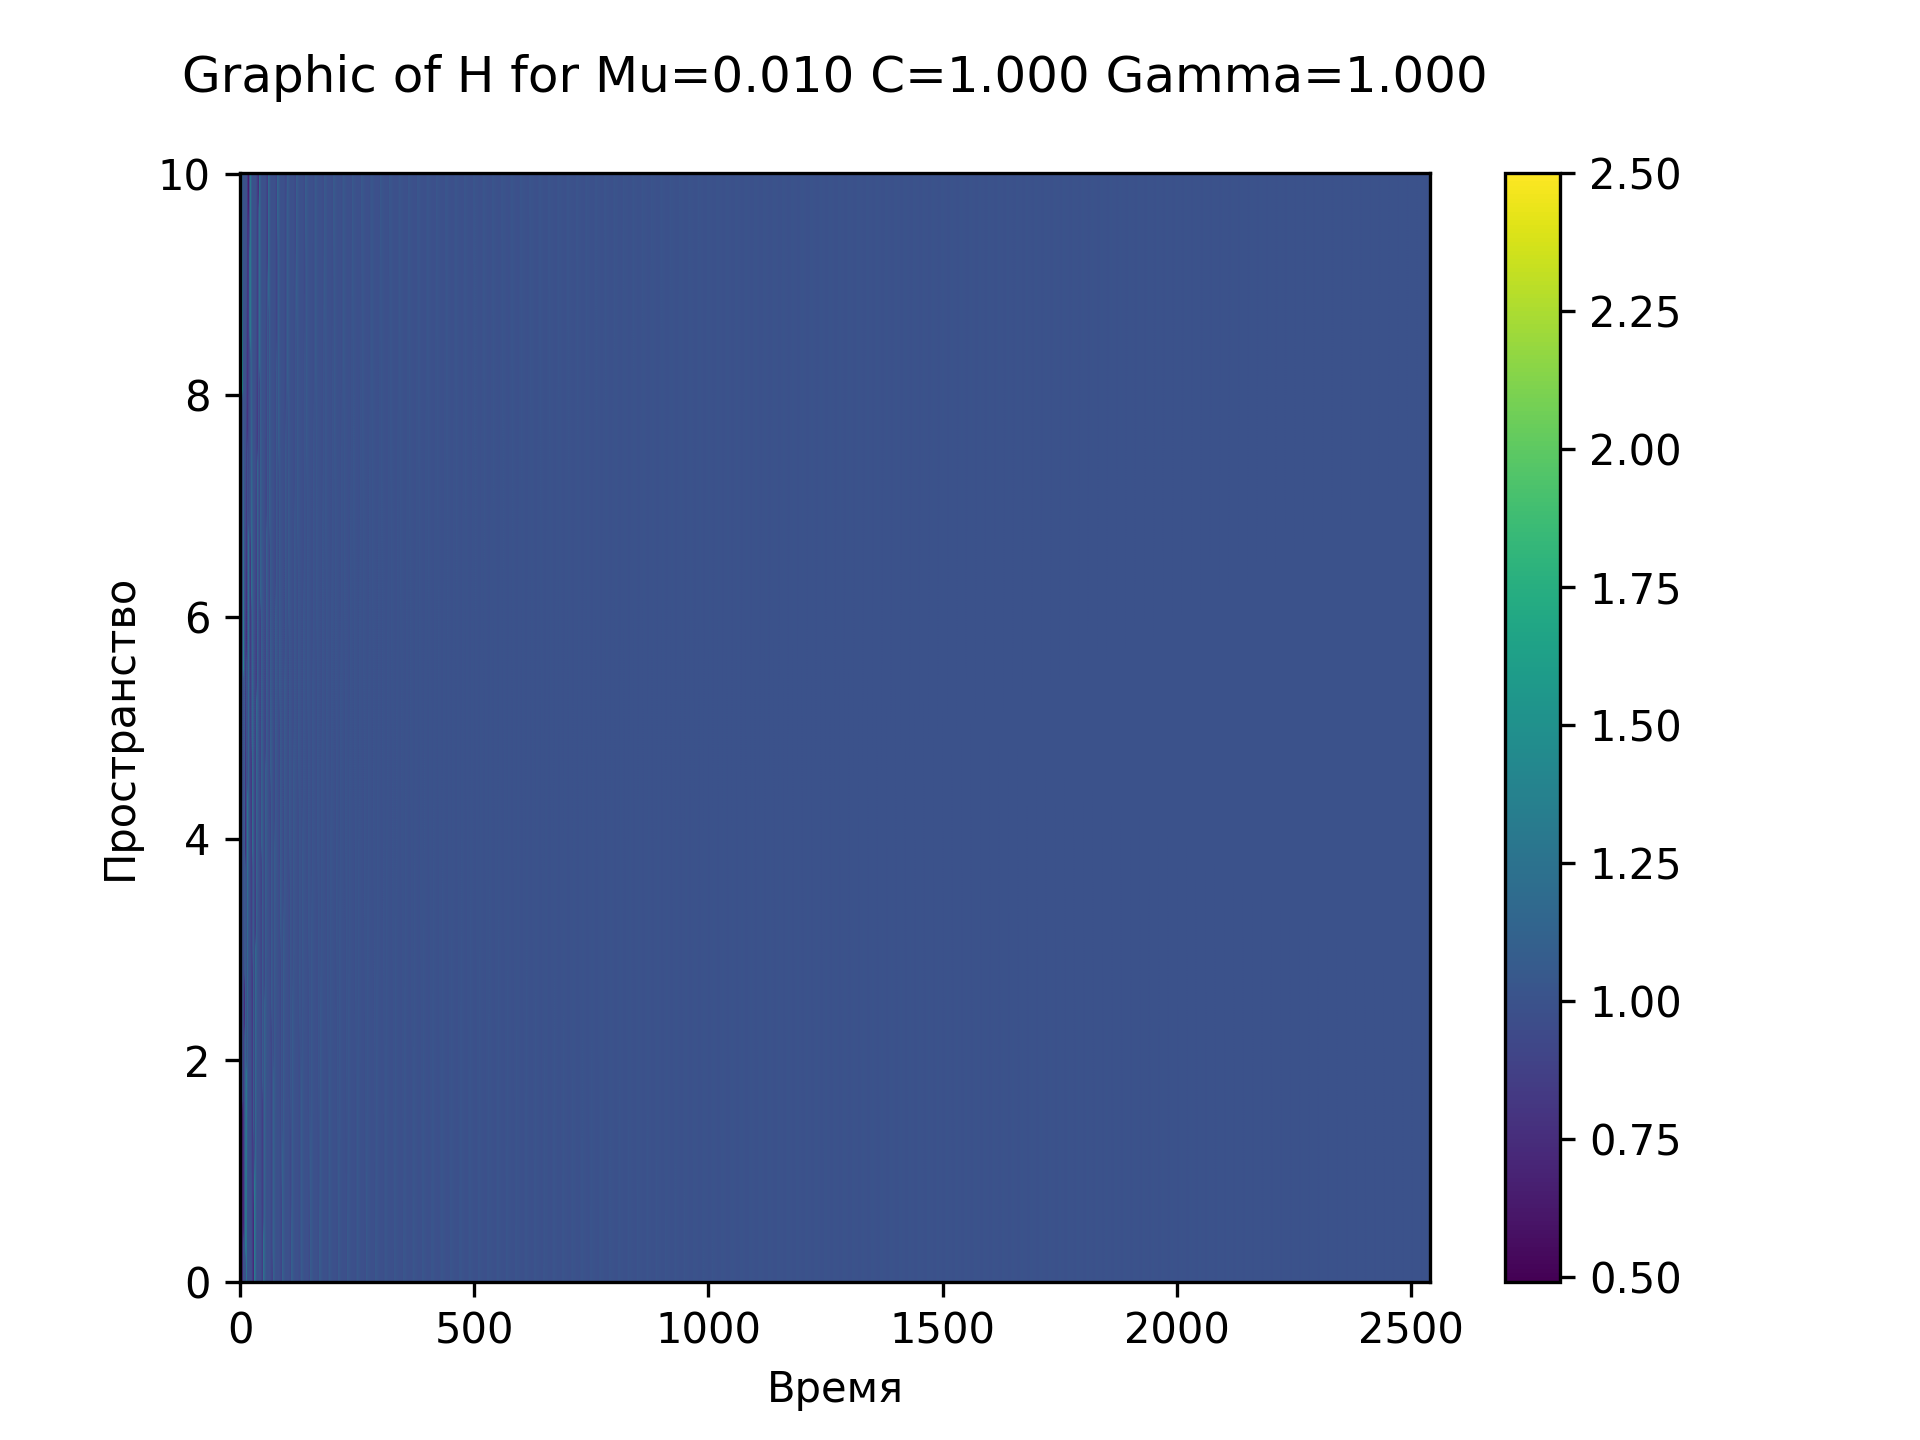
\includegraphics[scale=0.5]{../graphs_data_nonsmooth_2/value/Graph_H_mu0.010_C1.000_gamma1.000.png}
	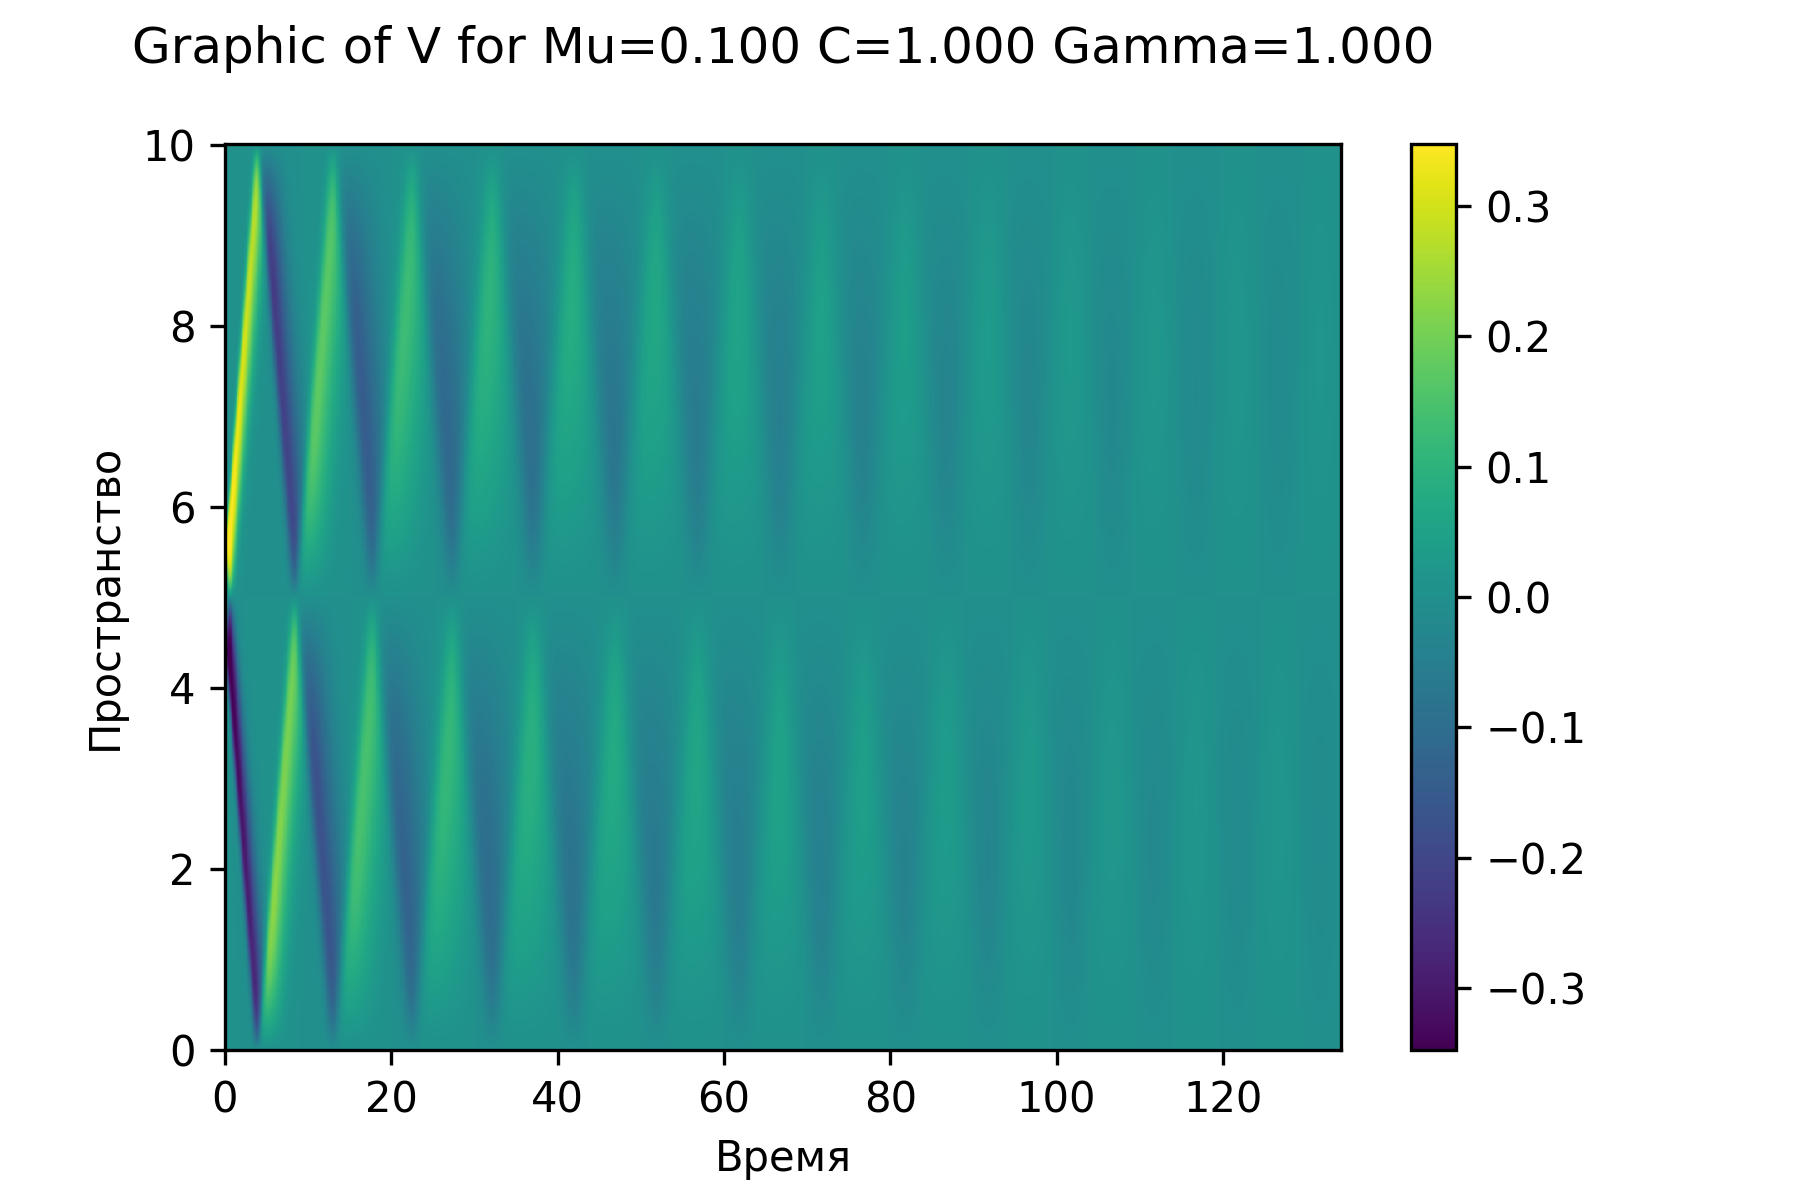
\includegraphics[scale=0.5]{../graphs_data_nonsmooth_2/value/Graph_V_mu0.010_C1.000_gamma1.000.png}	
	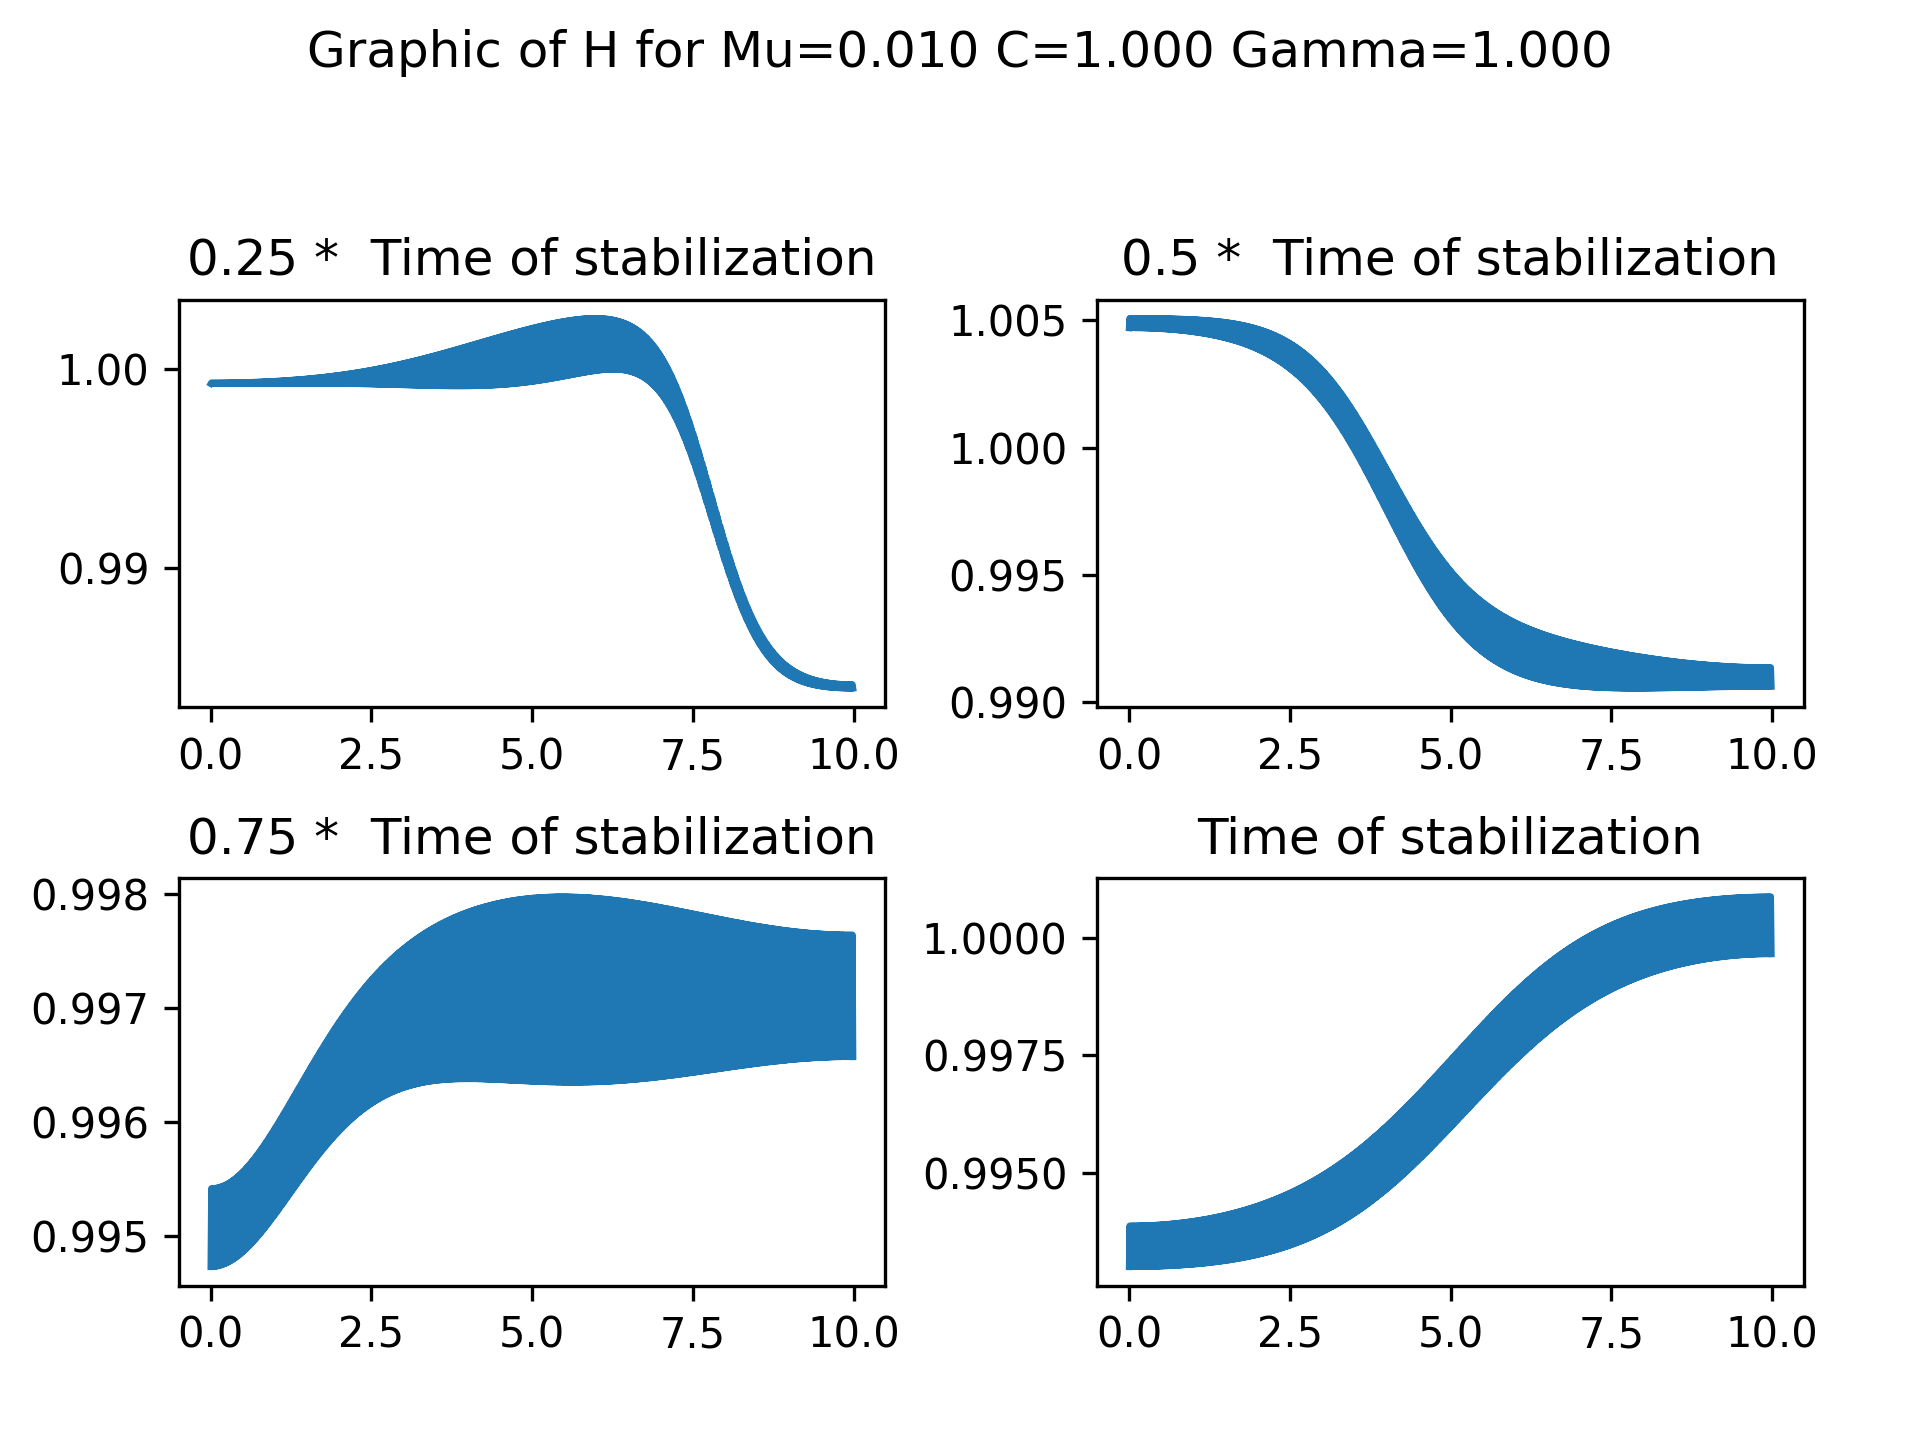
\includegraphics[scale=0.5]{../graphs_data_nonsmooth_2/slices/Graph_H_mu0.010_C1.000_gamma1.000.png}
	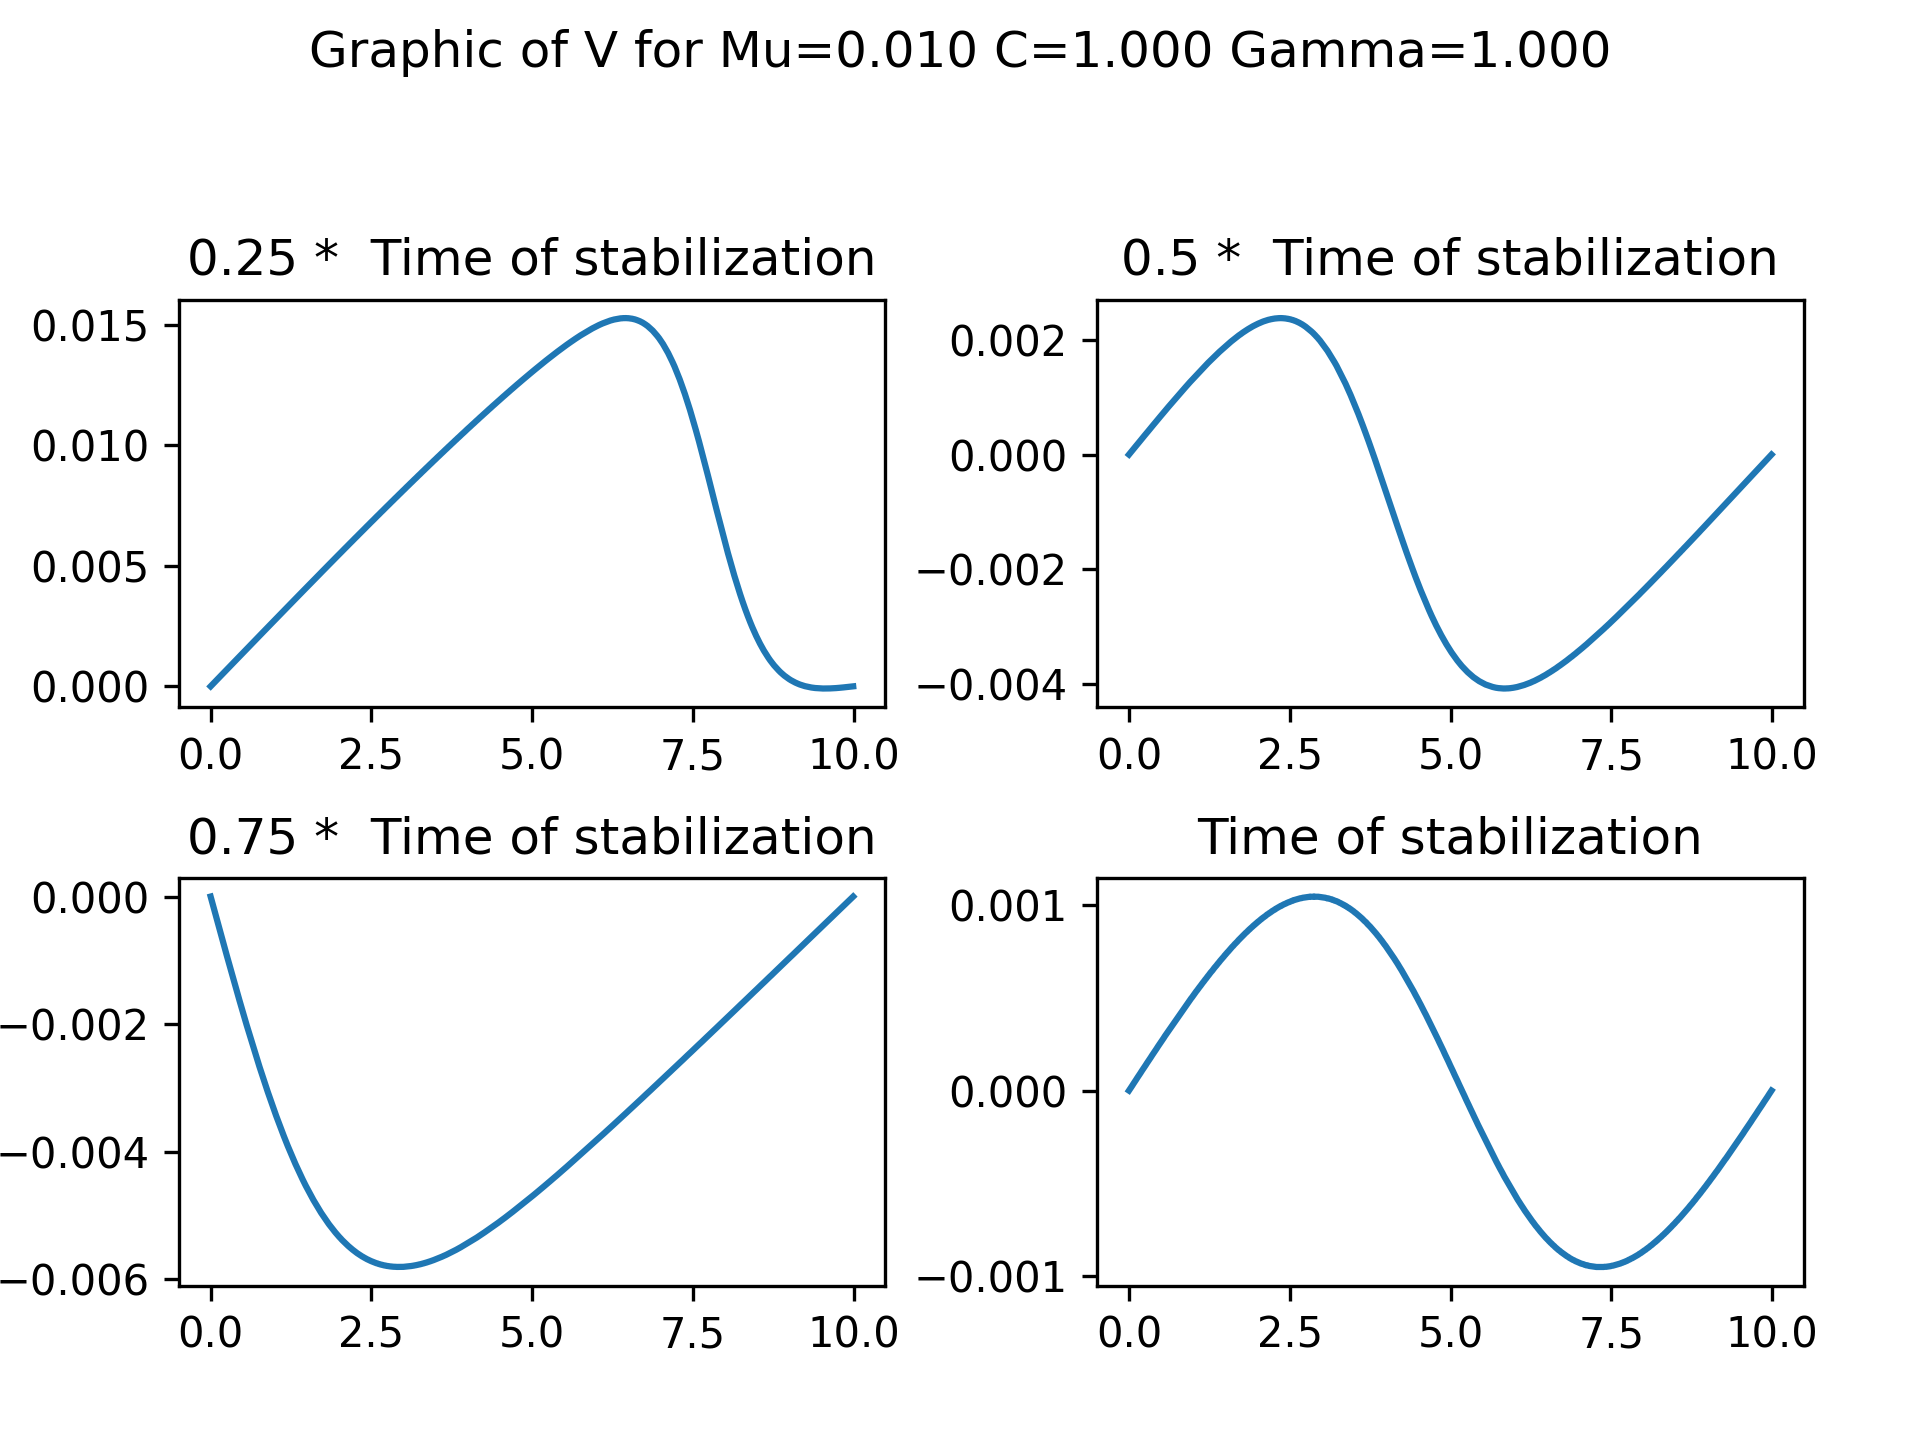
\includegraphics[scale=0.5]{../graphs_data_nonsmooth_2/slices/Graph_V_mu0.010_C1.000_gamma1.000.png}
\end{figure}

\begin{figure}[H]
	\centering
	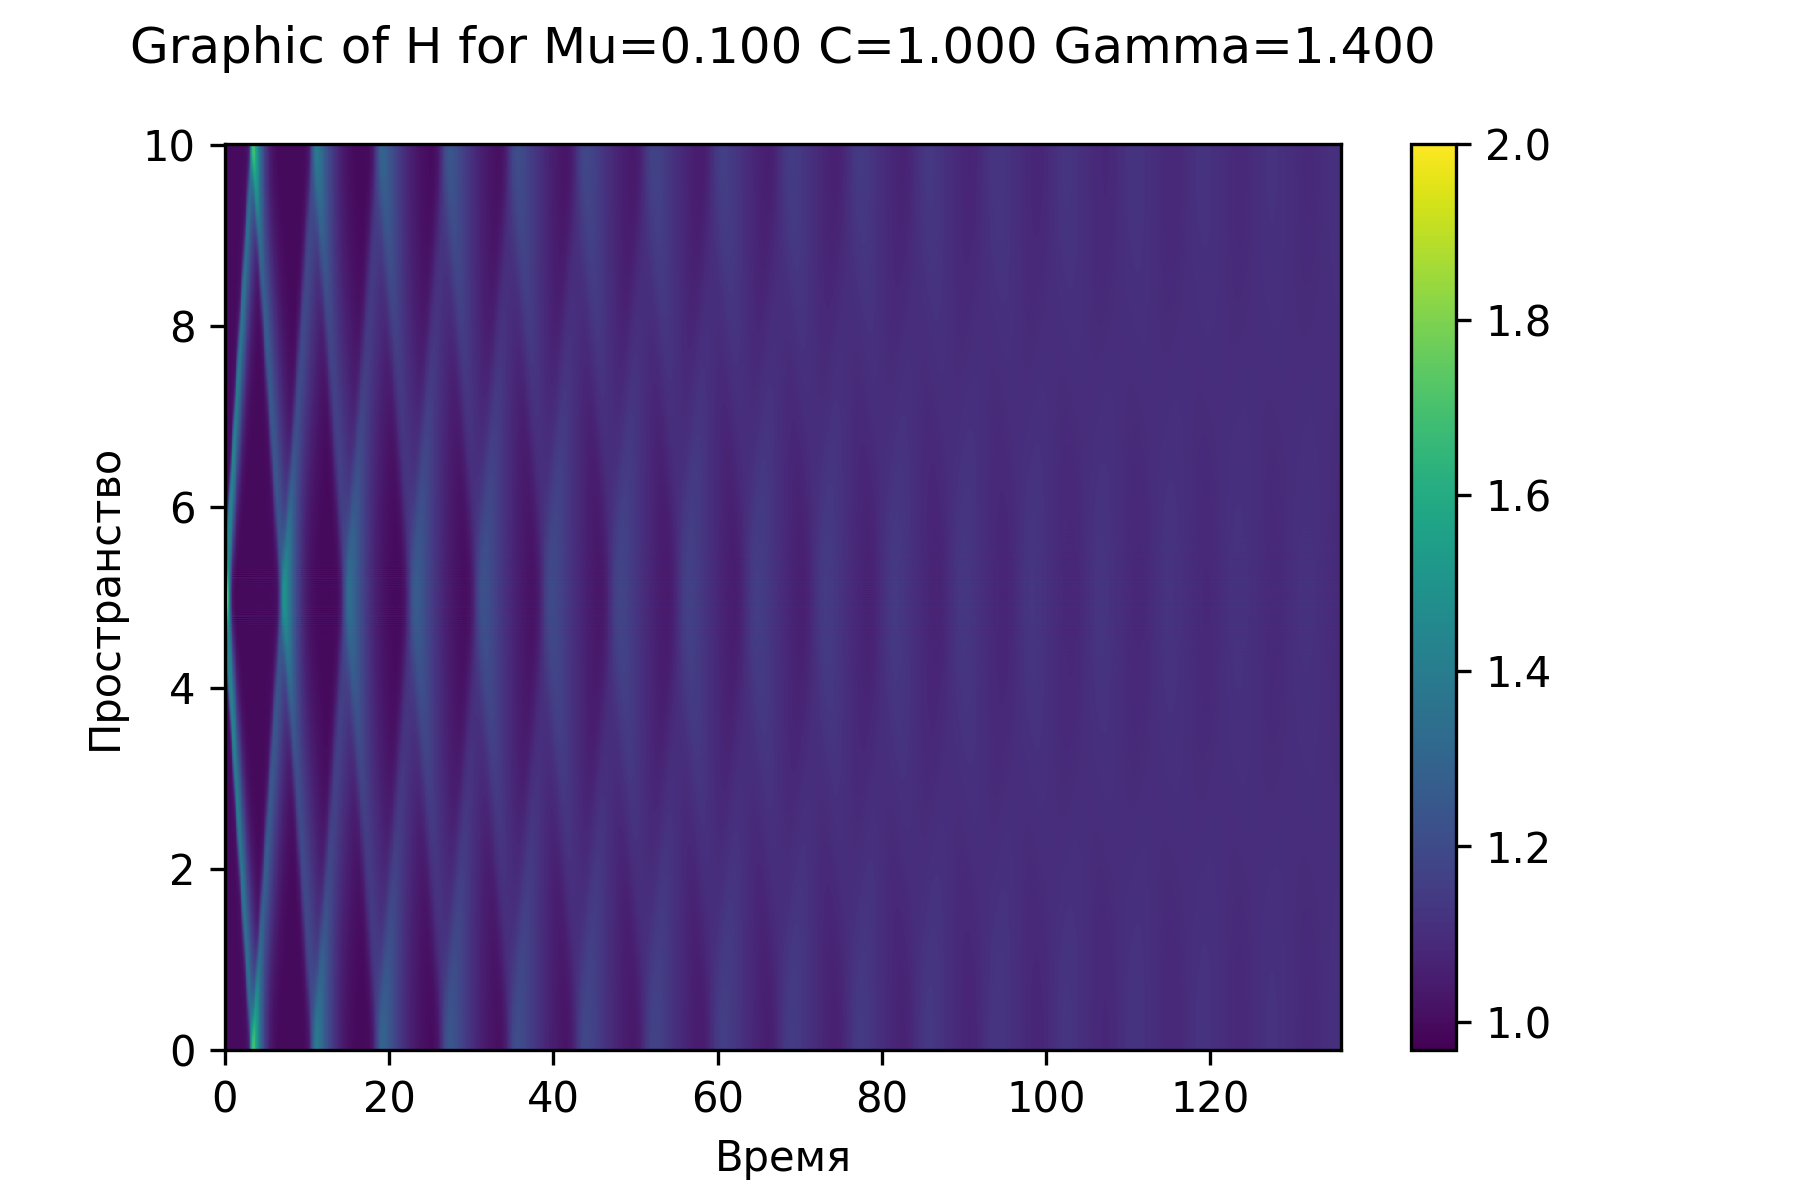
\includegraphics[scale=0.5]{../graphs_data_nonsmooth_2/value/Graph_H_mu0.010_C1.000_gamma1.400.png}
	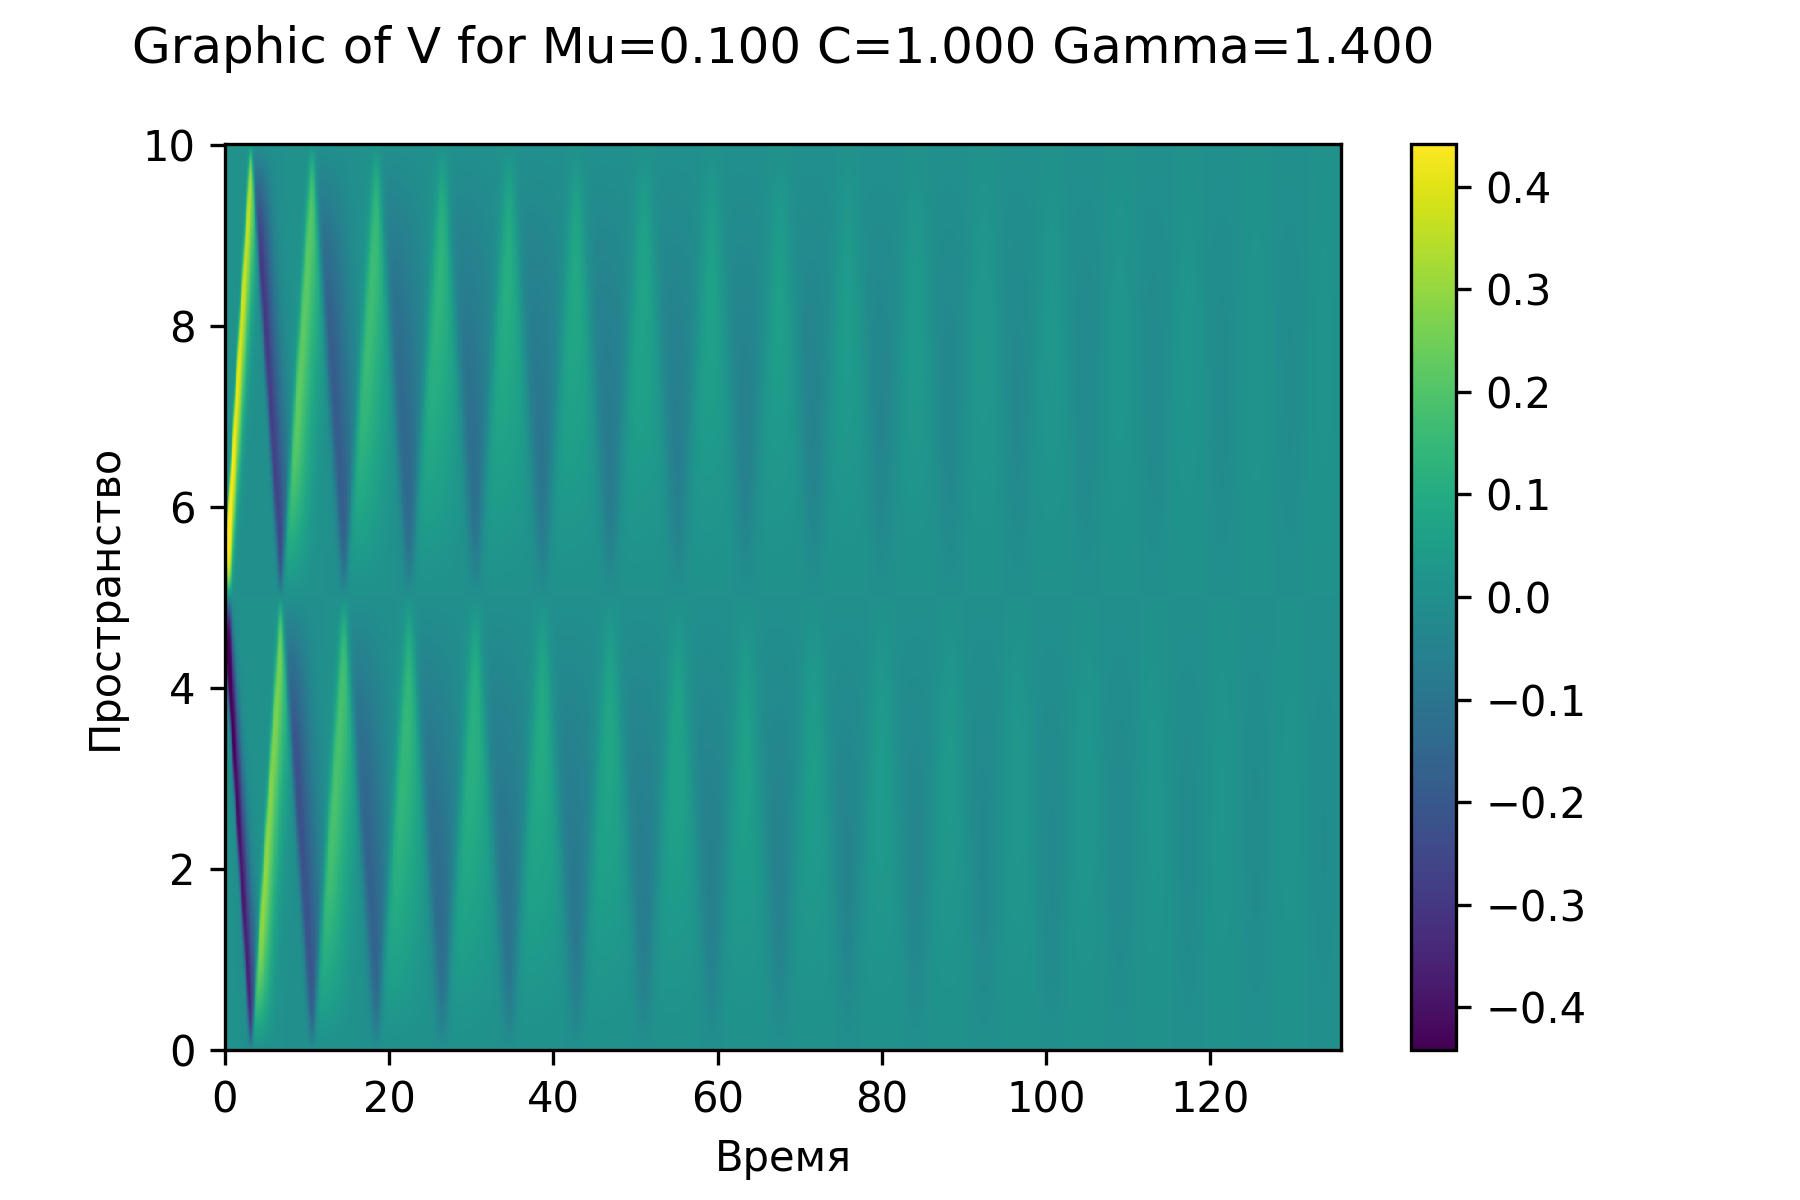
\includegraphics[scale=0.5]{../graphs_data_nonsmooth_2/value/Graph_V_mu0.010_C1.000_gamma1.400.png}	
	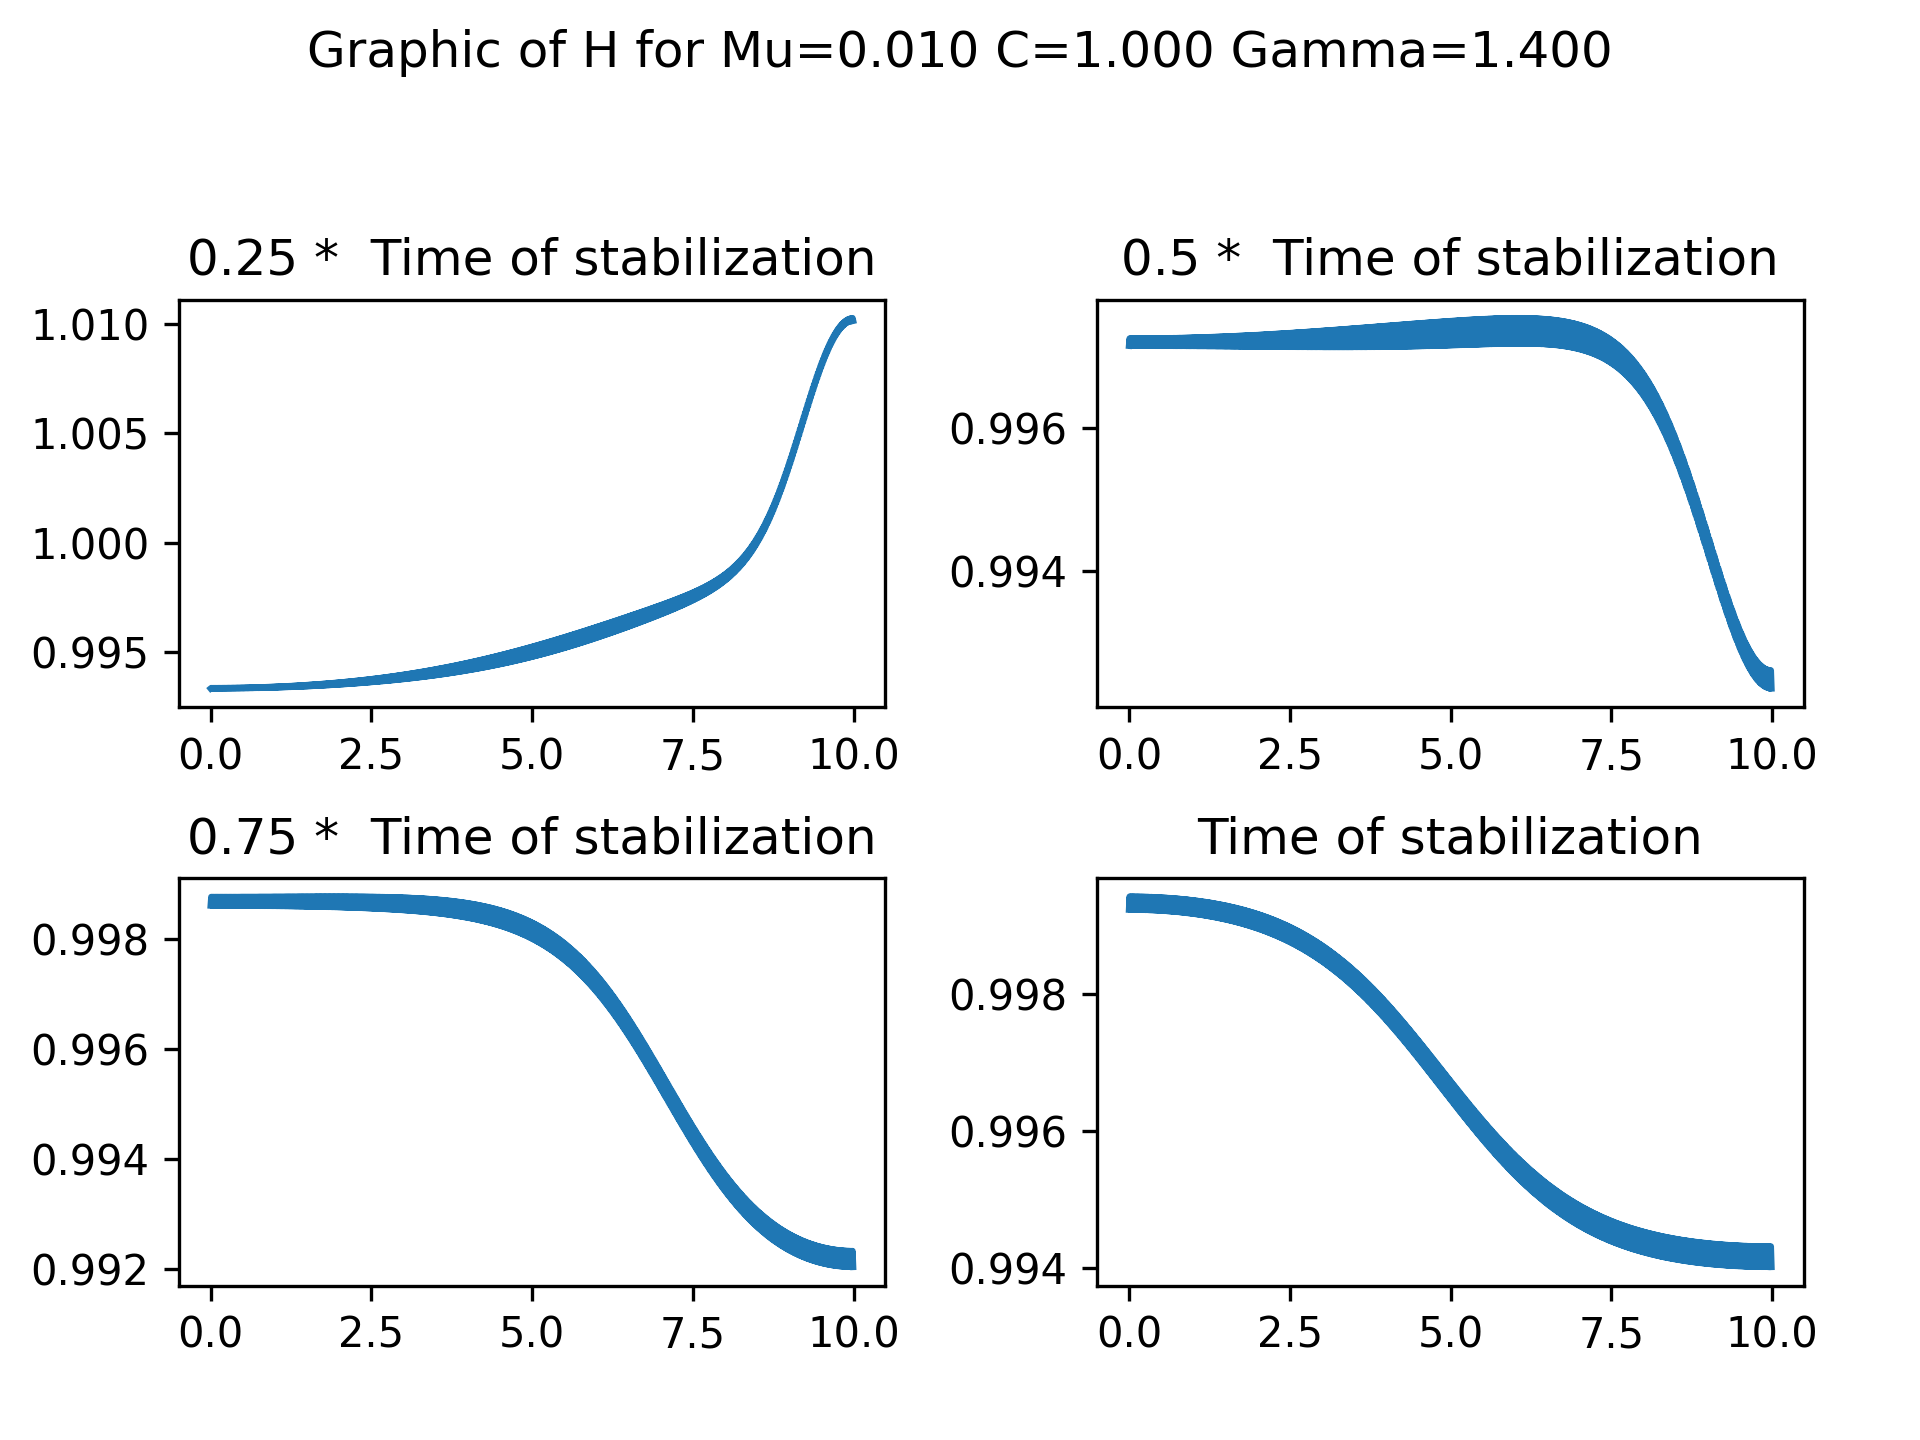
\includegraphics[scale=0.5]{../graphs_data_nonsmooth_2/slices/Graph_H_mu0.010_C1.000_gamma1.400.png}
	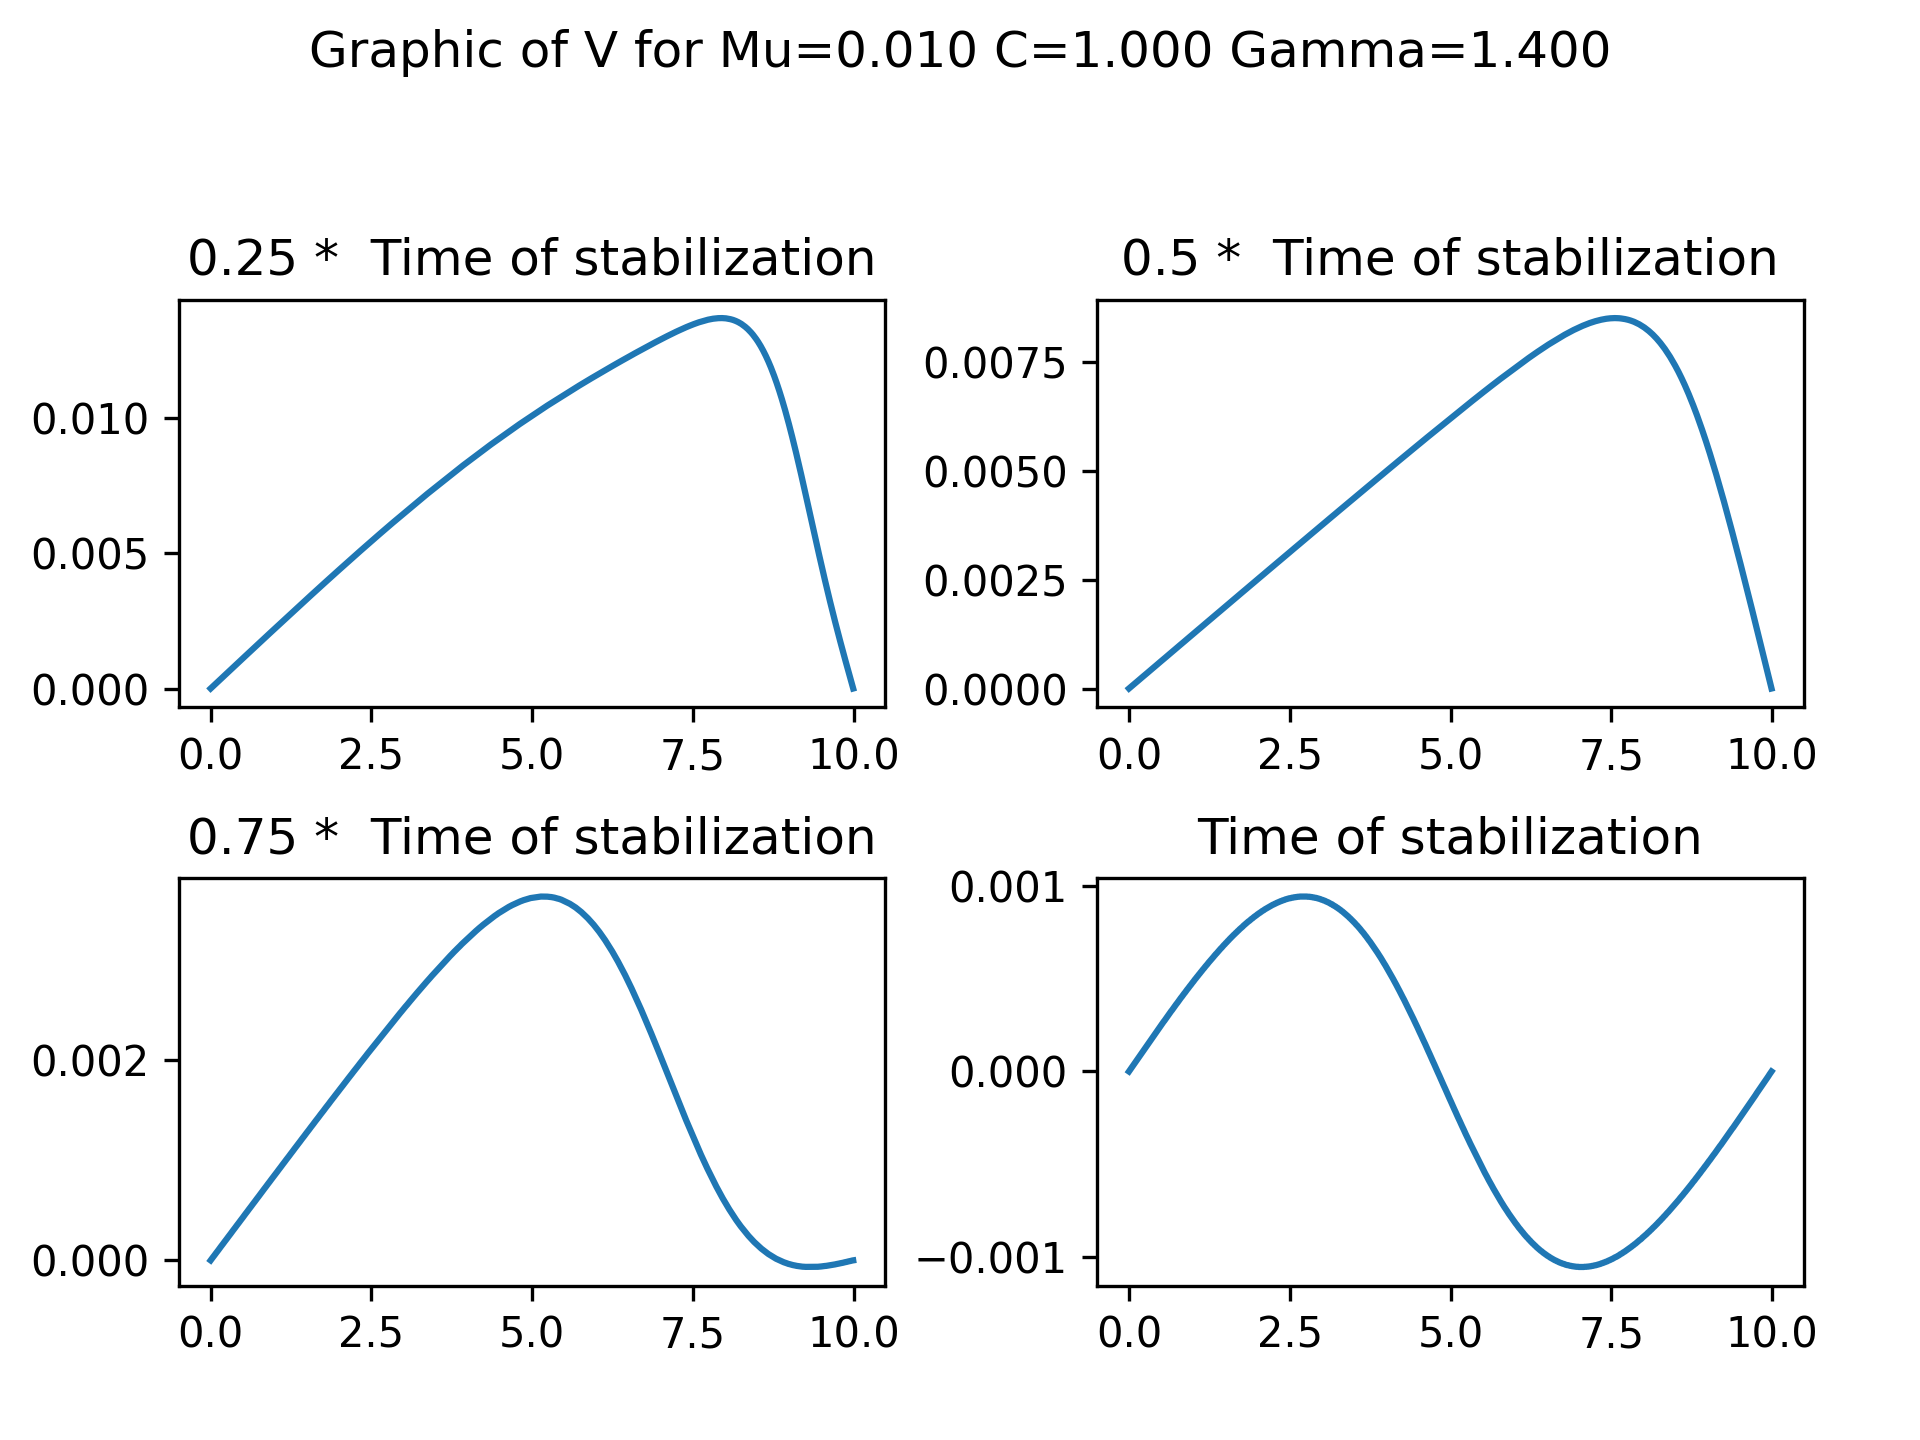
\includegraphics[scale=0.5]{../graphs_data_nonsmooth_2/slices/Graph_V_mu0.010_C1.000_gamma1.400.png}
\end{figure}

\begin{figure}[H]
	\centering
	\includegraphics[scale=0.5]{../graphs_data_nonsmooth_2/value/Graph_H_mu0.100_C10.000_gamma1.000.png}
	\includegraphics[scale=0.5]{../graphs_data_nonsmooth_2/value/Graph_V_mu0.100_C10.000_gamma1.000.png}	
	\includegraphics[scale=0.5]{../graphs_data_nonsmooth_2/slices/Graph_H_mu0.100_C10.000_gamma1.000.png}
	\includegraphics[scale=0.5]{../graphs_data_nonsmooth_2/slices/Graph_V_mu0.100_C10.000_gamma1.000.png}
\end{figure}

\begin{figure}[H]
	\centering
	\includegraphics[scale=0.5]{../graphs_data_nonsmooth_2/value/Graph_H_mu0.100_C1.000_gamma1.000.png}
	\includegraphics[scale=0.5]{../graphs_data_nonsmooth_2/value/Graph_V_mu0.100_C1.000_gamma1.000.png}	
	\includegraphics[scale=0.5]{../graphs_data_nonsmooth_2/slices/Graph_H_mu0.100_C1.000_gamma1.000.png}
	\includegraphics[scale=0.5]{../graphs_data_nonsmooth_2/slices/Graph_V_mu0.100_C1.000_gamma1.000.png}
\end{figure}

\begin{figure}[H]
	\centering
	\includegraphics[scale=0.5]{../graphs_data_nonsmooth_2/value/Graph_H_mu0.100_C1.000_gamma1.400.png}
	\includegraphics[scale=0.5]{../graphs_data_nonsmooth_2/value/Graph_V_mu0.100_C1.000_gamma1.400.png}	
	\includegraphics[scale=0.5]{../graphs_data_nonsmooth_2/slices/Graph_H_mu0.100_C1.000_gamma1.400.png}
	\includegraphics[scale=0.5]{../graphs_data_nonsmooth_2/slices/Graph_V_mu0.100_C1.000_gamma1.400.png}
\end{figure}

Период колебаний не зависит от $\mu$, однако при увеличении $C$ и $\gamma$ частота колебаний увеличивается. Однако при уменьшении $\mu$ увеличивается время стабилизации процесса.


\newpage
Приведем также графики невязок для различных параметров.
\begin{figure}[H]
	\centering
	\includegraphics[scale=0.65]{../graphs_data_nonsmooth_2/norms/Graph_V_norms_mu0.100_C10.000_gamma1.000.png}
	\includegraphics[scale=0.65]{../graphs_data_nonsmooth_2/norms/Graph_V_norms_mu0.100_C1.000_gamma1.000.png}	
	\includegraphics[scale=0.65]{../graphs_data_nonsmooth_2/norms/Graph_V_norms_mu0.100_C1.000_gamma1.400.png}
\end{figure}


\begin{figure}[H]
	\centering
	\includegraphics[scale=0.65]{../graphs_data_nonsmooth_2/norms/Graph_V_norms_mu0.010_C10.000_gamma1.000.png}
	\includegraphics[scale=0.65]{../graphs_data_nonsmooth_2/norms/Graph_V_norms_mu0.010_C1.000_gamma1.000.png}	
	\includegraphics[scale=0.65]{../graphs_data_nonsmooth_2/norms/Graph_V_norms_mu0.010_C1.000_gamma1.400.png}
\end{figure}

\newpage
Далее приведены значения $\Delta m(n)$ на измельченных и обычных сетках. А также их граффическое представление

\begin{center}
Table of mass loss. $\mu = 0.1000$ \, $C = 10.0000$, $\gamma = 1.0000$
  
\begin{tabular}{|p{0.8in}|p{0.8in}|p{0.8in}|p{0.8in}|p{0.8in}|p{0.8in}|p{0.8in}|} \hline
$K$ &$N_0$ &$N_0 \tau$ &$n = \frac{N_0}{4}$ &$n = \frac{N_0}{2}$ &$n = \frac{3N_0}{4}$ &$n = N_0$ \\ \hline 
0 &444220 &4.442e+02 &2.725e-04 &2.826e-04 &2.854e-04 &2.863e-04 \\ \hline 
1 &888439 &4.442e+02 &1.288e-04 &1.336e-04 &1.349e-04 &1.353e-04 \\ \hline 
2 &1776877 &4.442e+02 &6.272e-05 &6.505e-05 &6.568e-05 &6.586e-05 \\ \hline 
3 &3553753 &4.442e+02 &3.096e-05 &3.211e-05 &3.242e-05 &3.251e-05 \\ \hline 

\end{tabular}\\[20pt]
\end{center}

\begin{center}
Table of mass loss. $\mu = 0.1000$ \, $C = 1.0000$, $\gamma = 1.0000$
  
\begin{tabular}{|p{0.8in}|p{0.8in}|p{0.8in}|p{0.8in}|p{0.8in}|p{0.8in}|p{0.8in}|} \hline
$K$ &$N_0$ &$N_0 \tau$ &$n = \frac{N_0}{4}$ &$n = \frac{N_0}{2}$ &$n = \frac{3N_0}{4}$ &$n = N_0$ \\ \hline 
0 &414339 &4.143e+02 &2.568e-04 &2.822e-04 &2.735e-04 &2.757e-04 \\ \hline 
1 &828677 &4.143e+02 &1.273e-04 &1.399e-04 &1.357e-04 &1.367e-04 \\ \hline 
2 &1657353 &4.143e+02 &6.339e-05 &6.971e-05 &6.757e-05 &6.811e-05 \\ \hline 
3 &3314705 &4.143e+02 &3.164e-05 &3.479e-05 &3.373e-05 &3.400e-05 \\ \hline 

\end{tabular}\\[20pt]
\end{center}

\begin{center}
Table of mass loss. $\mu = 0.1000$ \, $C = 1.0000$, $\gamma = 1.4000$
  
\begin{tabular}{|p{0.8in}|p{0.8in}|p{0.8in}|p{0.8in}|p{0.8in}|p{0.8in}|p{0.8in}|} \hline
$K$ &$N_0$ &$N_0 \tau$ &$n = \frac{N_0}{4}$ &$n = \frac{N_0}{2}$ &$n = \frac{3N_0}{4}$ &$n = N_0$ \\ \hline 
0 &135888 &1.359e+02 &2.745e-04 &2.090e-04 &2.116e-04 &2.205e-04 \\ \hline 
1 &271775 &1.359e+02 &1.358e-04 &1.033e-04 &1.044e-04 &1.088e-04 \\ \hline 
2 &543549 &1.359e+02 &6.751e-05 &5.138e-05 &5.186e-05 &5.401e-05 \\ \hline 
3 &1087097 &1.359e+02 &3.366e-05 &2.562e-05 &2.584e-05 &2.691e-05 \\ \hline 

\end{tabular}\\[20pt]
\end{center}

\begin{center}
Table of mass loss. $\mu = 0.0100$ \, $C = 10.0000$, $\gamma = 1.0000$
  
\begin{tabular}{|p{0.8in}|p{0.8in}|p{0.8in}|p{0.8in}|p{0.8in}|p{0.8in}|p{0.8in}|} \hline
$K$ &$N_0$ &$N_0 \tau$ &$n = \frac{N_0}{4}$ &$n = \frac{N_0}{2}$ &$n = \frac{3N_0}{4}$ &$n = N_0$ \\ \hline 
0 &1482964 &1.483e+03 &3.484e-01 &3.484e-01 &3.484e-01 &3.484e-01 \\ \hline 
1 &2965927 &1.483e+03 &3.022e-02 &3.022e-02 &3.023e-02 &3.023e-02 \\ \hline 
2 &5931853 &1.483e+03 &7.440e-03 &7.443e-03 &7.443e-03 &7.443e-03 \\ \hline 
3 &11863705 &1.483e+03 &2.969e-03 &2.970e-03 &2.971e-03 &2.970e-03 \\ \hline 

\end{tabular}\\[20pt]
\end{center}

\begin{center}
Table of mass loss. $\mu = 0.0100$ \, $C = 1.0000$, $\gamma = 1.0000$
  
\begin{tabular}{|p{0.8in}|p{0.8in}|p{0.8in}|p{0.8in}|p{0.8in}|p{0.8in}|p{0.8in}|} \hline
$K$ &$N_0$ &$N_0 \tau$ &$n = \frac{N_0}{4}$ &$n = \frac{N_0}{2}$ &$n = \frac{3N_0}{4}$ &$n = N_0$ \\ \hline 
0 &2541366 &2.541e+03 &3.223e-03 &3.220e-03 &3.223e-03 &3.222e-03 \\ \hline 
1 &5082731 &2.541e+03 &1.481e-03 &1.479e-03 &1.480e-03 &1.480e-03 \\ \hline 
2 &10165461 &2.541e+03 &7.141e-04 &7.130e-04 &7.136e-04 &7.135e-04 \\ \hline 
3 &20330921 &2.541e+03 &3.511e-04 &3.505e-04 &3.508e-04 &3.508e-04 \\ \hline 

\end{tabular}\\[20pt]
\end{center}

\begin{center}
Table of mass loss. $\mu = 0.0100$ \, $C = 1.0000$, $\gamma = 1.4000$
  
\begin{tabular}{|p{0.8in}|p{0.8in}|p{0.8in}|p{0.8in}|p{0.8in}|p{0.8in}|p{0.8in}|} \hline
$K$ &$N_0$ &$N_0 \tau$ &$n = \frac{N_0}{4}$ &$n = \frac{N_0}{2}$ &$n = \frac{3N_0}{4}$ &$n = N_0$ \\ \hline 
0 &2495755 &2.496e+03 &3.307e-03 &3.316e-03 &3.316e-03 &3.315e-03 \\ \hline 
1 &4991509 &2.496e+03 &1.473e-03 &1.477e-03 &1.478e-03 &1.477e-03 \\ \hline 
2 &9983017 &2.496e+03 &7.009e-04 &7.028e-04 &7.031e-04 &7.030e-04 \\ \hline 
3 &19966033 &2.496e+03 &3.425e-04 &3.434e-04 &3.436e-04 &3.435e-04 \\ \hline 

\end{tabular}\\[20pt]
\end{center}


\newpage
\begin{figure}[H]
	\centering
	\includegraphics[scale=0.65]{../graphs_data_nonsmooth_2/mass/Graph_mass_mu0.100_C10.000_gamma1.000.png}
	\includegraphics[scale=0.65]{../graphs_data_nonsmooth_2/mass/Graph_mass_mu0.100_C1.000_gamma1.000.png}	
	\includegraphics[scale=0.65]{../graphs_data_nonsmooth_2/mass/Graph_mass_mu0.100_C1.000_gamma1.400.png}
\end{figure}


\begin{figure}[H]
	\centering
	\includegraphics[scale=0.65]{../graphs_data_nonsmooth_2/mass/Graph_mass_mu0.010_C10.000_gamma1.000.png}
	\includegraphics[scale=0.65]{../graphs_data_nonsmooth_2/mass/Graph_mass_mu0.010_C1.000_gamma1.000.png}	
	\includegraphics[scale=0.65]{../graphs_data_nonsmooth_2/mass/Graph_mass_mu0.010_C1.000_gamma1.400.png}
\end{figure}

Как можно заметить по таблицам потери массы составляют меньше 1-2\%, из чего можно заключить, что закон сохранения массы также выполняется. \\


